% This is the Reed College LaTeX thesis template. Most of the work
% for the document class was done by Sam Noble (SN), as well as this
% template. Later comments etc. by Ben Salzberg (BTS). Additional
% restructuring and APA support by Jess Youngberg (JY).
% Your comments and suggestions are more than welcome; please email
% them to cus@reed.edu
%
% See http://web.reed.edu/cis/help/latex.html for help. There are a
% great bunch of help pages there, with notes on
% getting started, bibtex, etc. Go there and read it if you're not
% already familiar with LaTeX.
%
% Any line that starts with a percent symbol is a comment.
% They won't show up in the document, and are useful for notes
% to yourself and explaining commands.
% Commenting also removes a line from the document;
% very handy for troubleshooting problems. -BTS

% As far as I know, this follows the requirements laid out in
% the 2002-2003 Senior Handbook. Ask a librarian to check the
% document before binding. -SN

%%
%% Preamble
%%
% \documentclass{<something>} must begin each LaTeX document
\documentclass[12pt,oneside]{psthesis}
% Packages are extensions to the basic LaTeX functions. Whatever you
% want to typeset, there is probably a package out there for it.
% Chemistry (chemtex), screenplays, you name it.
% Check out CTAN to see: http://www.ctan.org/
%%
\usepackage{graphicx,latexsym}
\usepackage{subfig}
\usepackage{amsmath}
\usepackage{amssymb,amsthm}
\usepackage{longtable,booktabs,setspace}
\usepackage[none]{hyphenat}
\PassOptionsToPackage{hyphens}{url}\usepackage[hidelinks,breaklinks]{hyperref}
% Added by CII
\usepackage{lmodern}
\usepackage{float}
\usepackage{titlesec}
\floatplacement{figure}{H}
% End of CII addition
\usepackage{rotating}
\usepackage{epigraph}
\usepackage{dcolumn}

% Next line commented out by CII
%%% \usepackage{natbib}
% Comment out the natbib line above and uncomment the following two lines to use the new
% biblatex-chicago style, for Chicago A. Also make some changes at the end where the
% bibliography is included.
%\usepackage{biblatex-chicago}
%\bibliography{thesis}


% Added by CII (Thanks, Hadley!)
% Use ref for internal links
\renewcommand{\hyperref}[2][???]{\autoref{#1}}
\def\chapterautorefname{Chapter}
\def\sectionautorefname{Section}
\def\subsectionautorefname{Subsection}
% End of CII addition

% Added by CII
\usepackage[font=singlespacing]{caption}
\captionsetup{margin=10pt}
% End of CII addition

% \usepackage{times} % other fonts are available like times, bookman, charter, palatino

% Syntax highlighting #22

% To pass between YAML and LaTeX the dollar signs are added by CII
\title{Political Impacts of Residential Mortgages in Crisis}
\author{Corey Runkel}
\computingid{\href{mailto:cnr3cg@virginia.edu}{\nolinkurl{cnr3cg@virginia.edu}}}
% The month and year that you submit your FINAL draft TO THE LIBRARY (May or December)
\date{20 April 2020}
\advisor{Herman M. Schwartz}
\institution{University of Virginia}
\degree{Bachelor of Arts with honors}
%If you have two advisors for some reason, you can use the following
% Uncommented out by CII
% End of CII addition

%%% Remember to use the correct department!
\department{Program in Political \& Social Thought}
% if you're writing a thesis in an interdisciplinary major,
% uncomment the line below and change the text as appropriate.
% check the Senior Handbook if unsure.
%\thedivisionof{The Established Interdisciplinary Committee for}
% if you want the approval page to say "Approved for the Committee",
% uncomment the next line
%\approvedforthe{Committee}

% Added by CII
%%% Copied from knitr
%% maxwidth is the original width if it's less than linewidth
%% otherwise use linewidth (to make sure the graphics do not exceed the margin)
\makeatletter
\def\maxwidth{ %
  \ifdim\Gin@nat@width>\linewidth
    \linewidth
  \else
    \Gin@nat@width
  \fi
}
\makeatother

\renewcommand{\contentsname}{Table of Contents}
% End of CII addition

\setlength{\parskip}{0pt}

% Added by CII

\providecommand{\tightlist}{%
  \setlength{\itemsep}{0pt}\setlength{\parskip}{0pt}}


\Abstract{
The mortgage crisis of 2007--2012 saw the foreclosure of some 10 million Americans.
In response, the federal government authorized three rounds of the Neighborhood Stabilization Program (NSP), a relief effort aimed at stabilizing prices and preventing further social discloation.
The program operated by purchasing, repairing, and re-selling vacant homes in neighborhoods at high risk of even more foreclosures.
Though this program resembled Democrat-supported welfare programs, there are theoretical questions about the impacts it may have had on voting.
Broadly, political economists have predicted that increased home equity leads to preferences for less social insurance, while early 21st-century American politics consistently connected less social insurance with lower taxation.
These features would suggest that the Neighborhood Stabilization Program pushed voters towards Republican candidates, especially towards self-avowed members of the Tea Party Caucus, which sharpened the taxation--social insurance connection and derided the subsidy of home mortgages.
I create a novel dataset connecting NSP target areas, 2010 midterm vote returns, home prices, and a range of demographic information in order to analyze this question.
I find some evidence that the behavior theorized did occur among races featuring a Tea Party candidate, but that the behavior stayed local to those races and was not a broader feature of Republican support.
}

	\usepackage{booktabs}
\usepackage{longtable}
\usepackage{array}
\usepackage{multirow}
\usepackage{wrapfig}
\usepackage{float}
\usepackage{colortbl}
\usepackage{pdflscape}
\usepackage{tabu}
\usepackage{threeparttable}
\usepackage{threeparttablex}
\usepackage[normalem]{ulem}
\usepackage{makecell}
\usepackage{xcolor}
% End of CII addition
%%
%% End Preamble
%%
%
\begin{document}

% Everything below added by CII
  \maketitle

\frontmatter % this stuff will be roman-numbered

  \setcounter{tocdepth}{2}
  \tableofcontents
  \thispagestyle{plain} % this removes page numbers from the frontmatter

  \listoftables
  \thispagestyle{plain} % this removes page numbers from the frontmatter

  \listoffigures
  \thispagestyle{plain} % this removes page numbers from the frontmatter
  \begin{abstract}
  \thispagestyle{plain} % this removes page numbers from the frontmatter
  \doublespacing
    The mortgage crisis of 2007--2012 saw the foreclosure of some 10 million Americans.
    In response, the federal government authorized three rounds of the Neighborhood Stabilization Program (NSP), a relief effort aimed at stabilizing prices and preventing further social discloation.
    The program operated by purchasing, repairing, and re-selling vacant homes in neighborhoods at high risk of even more foreclosures.
    Though this program resembled Democrat-supported welfare programs, there are theoretical questions about the impacts it may have had on voting.
    Broadly, political economists have predicted that increased home equity leads to preferences for less social insurance, while early 21st-century American politics consistently connected less social insurance with lower taxation.
    These features would suggest that the Neighborhood Stabilization Program pushed voters towards Republican candidates, especially towards self-avowed members of the Tea Party Caucus, which sharpened the taxation--social insurance connection and derided the subsidy of home mortgages.
    I create a novel dataset connecting NSP target areas, 2010 midterm vote returns, home prices, and a range of demographic information in order to analyze this question.
    I find some evidence that the behavior theorized did occur among races featuring a Tea Party candidate, but that the behavior stayed local to those races and was not a broader feature of Republican support.
  \end{abstract}

\mainmatter % here the regular arabic numbering starts
\pagestyle{fancyplain} % turns page numbering back on
\doublespacing
\titleformat{\chapter}[display]{\normalfont\huge\bfseries\singlespacing}{\chaptertitlename\ \thechapter}{40pt}{\huge}
\titleformat{\section}{\singlespacing\normalfont\Large\bfseries}{\thesection}{1em}{}
\titleformat{\subsection}{\singlespacing\normalfont\large\bfseries}{\thesubsection}{1em}{}
\titleformat{\subsubsection}{\singlespacing\normalfont\normalsize\bfseries}{\thesubsubsection}{1em}{}

\hypertarget{actors-motive}{%
\chapter{Introduction}\label{actors-motive}}

Between 2007 and 2012, 10 million Americans---1 of every 20 adults---lost their homes.\footnote{Isaac William Martin and Christopher Niedt, \emph{Foreclosed America} (Stanford, California: Stanford University Press, 2015).}
It was clear then that homeowners needed an intervention.
When Countrywide, which two years earlier had serviced 20\% of the mortgages in the United States,\footnote{Herman M. Schwartz and Leonard Seabrooke, eds., \emph{The Politics of Housing Booms and Busts}, International Political Economy Series (Palgrave Macmillan UK, 2009), \url{https://doi.org/10.1057/9780230280441}.} collapsed in July 2008, it was clear that the real estate industry needed to change.
When cities and counties around California, Florida, Nevada, and Arizona trembled at a declining tax base, it was clear that municipalities needed a break.
Yet, none of these actors wielded much power in the response to the subprime mortgage crisis.
Unlike the Great Depression, homeowners barely organized their political power and financial institutions imposed very modest debtor-relief programs.
Additionally, the long-term trend of municipal disinvestment emphasized the need to remove neighborhood blight instead of create or subsidize housing.

In response, the Housing and Economic Recovery Act of 2008 (HERA) authorized the Department of Housing and Urban Development (HUD) to distribute \$3.9 billion to state and local governments for the purchase and repair of foreclosed properties.\footnote{Nancy Pelosi, ``Housing and Economic Recovery Act of 2008,'' July 2008.}
This program, later termed the Neighborhood Stabilization Program (NSP), is my focus.
In purchasing, repairing, and in most cases reselling foreclosed properties, the NSP sought to mitigate the effects of foreclosures on their surroundings.
Primarily, foreclosures tear people from their homes.
On top of this comes the stigma of being a ``deadbeat''\footnote{David Dayen, \emph{Chain of Title: How Three Ordinary Americans Uncovered Wall Street's Great Foreclosure Fraud} (New York: The New Press, 2016).} and mounds of fees---legal, cancellation, transportation-related.
But once homeowners have been forced out, the neighborhood and municipality bear the financial weight of that foreclosure.

This thesis considers two lines of analysis, the first a question of method and mechanism, the second a question of politics and historical contingency.
These two lines converge with the Neighborhood Stabilization Program amid the rise of the Tea Party.
The first attempts to add to the political science and sociology literature around the connections between housing, political preferences, and voting.
This line of analysis is motivated by the opportunity presented by the Neighborhood Stabilization Program, 2010 decennial census, and 2010 midterm elections to bridge a gap in the measurement of political behavior.
While the first two components offer unusually granular and contemporary data, the midterm elections posed a unique brand of politics to American voters.
This brand of politics was neither usual nor inevitable, an observation I take great pains to make in Chapter \ref{motive-opportunity}.
Rather, it was a product of the political and economic mechanisms investigated by the literature I engage methodologically in my first line of analysis.
The historical claims are not new; they have been fashioned directly from the work of others.
I zoom in on a particular corner of political economy and housing, however, to beef up my methodological assumptions.
The relationship between these two lines of analysis is complex but understanding it is imperative to comprehending the validity of my argument about the impact of the Neighborhood Stabilization Program.

To nearby homeowners, foreclosures cost \$159,000 on average in decreased property values.\footnote{Daniel Immergluck, \emph{Foreclosed: High-Risk Lending, Deregulation, and the Undermining of America's Mortgage Market} (Ithaca: Cornell University Press, 2011), 151.}
To the city or county that envelops the property, it costs around \$50,000 for the legal and construction work to demolish and resell a vacant lot, parcels which tend to drop property values even further.\footnote{Daniel Indiviglio, ``The Housing Stabilization Program You Haven't Heard About,'' \emph{The Atlantic} (https://www.theatlantic.com/business/archive/2010/04/the-housing-stabilization-program-you-havent-heard-about/38739/, April 2010).}
When property values drop, a home's {[}apparent{]} equity drops too.
This figure, estimated constantly by market research firms such as Zillow and appraised periodically by taxing authorities, determines to a large extent the wealth and borrowing power of homeowners.
If the value of an already-mortgaged home rises, homeowners can refinance.
While refinancing most often takes advantage of lower interest rates or decreased principal amounts to reduce monthly payments, refinancing was used by in the lead up to the subprime mortgage crisis instead to finance renovations, service debts (eg. student, credit card, and car loans), or cash out.
Lending institutions willingly converted apparent value into real value, and as long as home values crept up, refinancing was viable.
This use of refinancing reflected a shift in how Americans approached housing, from the home as an utterly private good, to the home as an asset.
Homes stand increasingly in the position of pension plans and 401ks; a wise move can transform forty years into four-hundred thousand dollars.

These wise moves seemed to occur constantly from September 1992 until March 2006.
As Figure \ref{fig:caseshiller} shows, the intervening 14 years never once saw a drop in the industry's standard home-price metric, the Case-Shiller U.S. National Home Price Index.
As prices rose, homeowners refinanced, effectively paying back the first mortgage while taking out the second.
To investors in mortgage-backed securities (MBS), pre-payment from refinancing is usually seen as a risk, but constant and predictable refinancing added to the safety of securitization, playing into investors risk-reward calculus.
However, when prices fell---or even flatlined---this safety evaporated.
Without the increased {[}apparent{]} home equity, refinancing did nothing.
Falling prices thus meant homeowners were saddled with their current mortgage, often one whose interest rates reset after two years, climbing an interest-rate staircase for the next 28 years.
Atop the interest payments, living expenses (such as other debts) piled on to borrowers, where previously refinancing had arrived to supplement existing income with cash.
Falling prices meant homeowners chose among food, water, and shelter, if they had enough income for that to even be a decision.
\begin{figure}

{\centering 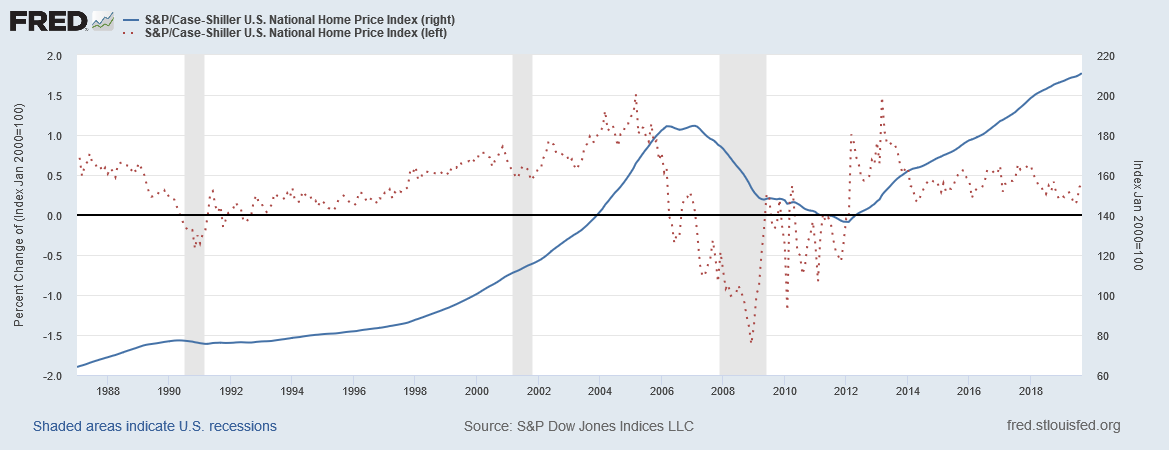
\includegraphics[width=0.9\linewidth]{figure/caseshiller_1990_2018} 

}

\caption{Price (right axis) and growth (left axis) of the Case-Shiller Home Price Index, adjusted for seasonal price fluctuations.}\label{fig:caseshiller}
\end{figure}
These factors make homeowners \emph{very} sensitive to falling or stagnant home prices.
In their sensitivity, they may have voted for parties, candidates, and policies they believed would drive up home prices, such as property tax cuts, muscular code enforcement, and spacious zoning regulations.
Each of these policies reduces the resources available for non-homeowners, pitting homeowners against renters, the homeless, and anyone else without a direct financial stake in the asset.
For example, tax cuts, take they the form of directly-decreased property taxes or the homeowner tax credit, reduce the monies available to fund public goods.
``Housing elements of the U.S. welfare state,'' Schwartz \& Seabrooke note, ``favor everyone but the `poor.'\,''\footnote{Schwartz and Seabrooke, \emph{The Politics of Housing Booms and Busts}, 212.}
The rigidity of these ideologies rationalizes the fear that rents extracted from higher taxation will not return to the homeowners.
Circling back to the original home-price dynamic, higher home values fund greater consumption, while lower property values and higher taxes (as they always have) limit homeowners' capacities to spend, an activity Americans very much enjoy.

When prices rose, creditor and debtor interests laid at some angle, intersecting in the particular case of safe, two-year refinancing, but divergent in the general case of refinancing that took advantage of lower interest rates.
On the other hand, falling housing prices conformed the immediate interests of creditors and debtors to one another, since delinquency and default eliminated any chance of extracting further rents.
Fears of a debt spiral triggered by falling home prices also beset cities,\footnote{Mark Muro and Christopher Hoene, ``Fiscal Challenges Facing Cities: Implications for Recovery'' (Brookings, November 2009).} though there is some doubt that those fears were justified.\footnote{Liz Gross et al., ``The Local Squeeze: Falling Revenues and Growing Demand for Services Challenge Cities, Counties, and School Districts,'' ed. Susan Urahn (Philadelphia: Pew Research Center, 2012); Byron Lutz, Raven Molloy, and Hui Shan, ``The Housing Crisis and State and Local Government Tax Revenue: Five Channels,'' \emph{Regional Science and Urban Economics}, Special Issue: The Effect of the Housing Crisis on State and Local Governments, 41, no. 4 (July 2011): 306--19, \url{https://doi.org/10.1016/j.regsciurbeco.2011.03.009}.}
With these interests in syzygy, why didn't homeowners, investors, or cities assert solutions, even ones that were done chiefly in their own interest?
I argue in this chapter first that homeowners remained quiet due to changes in the foreclosure process from the Great Depression, the differential character of housing versus farming, and narratives about mortgage debtors.
Second, the incongruity---spurred by the demise of savings and loans---between incentives for principals in mortgage-backed securities and agents tasked with servicing the underlying mortgages, along with fraudulent mortgage transfers, resulted in foreclosures that may have otherwise been unwanted by creditors.
Third, I point to municipal disinvestment and the trajectory of the Commerce Clause as reasons why cities were unable to handle mass foreclosures.
This critique I believe to be sufficient, though by no means necessary, to explaining why each was functionally barred from substantial action.

This argument serves dual purposes.
First, it justifies the motives of actors external to the creation of the Neighborhood Stabilization Program, to which internal actors, such as George W. Bush and members of Congress, responded.
Second, it offers a story about why external actors may not have acted decisively.
Readers should come away from this chapter understanding why federal foreclosure relief programs were necessary.

\hypertarget{homeowners}{%
\section{Why Homeowners were Unable to Organize}\label{homeowners}}

Reasons for the powerlessness of anti-foreclosure organizing can be shown through comparison with the most successful anti-foreclosure campaigns of the Great Depression.
Legislative movements require a base of public opinion and support, a mouthpiece through which opinion can be articulated, and an powerful audience to hear those articulated opinions and demands.
Foreclosed housing's base of public opinion and support was attenuated by geographic particularities of subprime mortgages which limited fora for communication, both internally and externally.
In addition, the organizers' audience was blocked partially by other demands, including the presence of mortgage servicers.
The Great Depression, however, saw these factors come together in the Midwest, where farms were physically parched and thus, financially underwater.
Farmers were positioned similar to homeowners who adopted cash-out refinancing in that they relied on their land for its income.

However, farmers in the Great Depression differed from early 2000s subprime borrowers in that farming did not \emph{supplement} wage income, it \emph{replaced} wage incomes.
In addition, access to government and stark differences in media portrayal combined with the larger impact of farm foreclosures to drive organizing that led to 27 states enacting \emph{per se} or \emph{de facto} moratoria on foreclosures.\footnote{David C Wheelock, ``Changing the Rules: State Mortgage Foreclosure Moratoria During the Great Depression,'' \emph{Federal Reserve Bank of St. Louis Review} 90, no. 6 (n.d.): 537.}
The lack of such conditions pitched the struggle for foreclosure legislation in the subprime mortgage crisis to a severe angle.

The most important differentiator between the foreclosure crisis in the Great Depression and that which preceded the Great Recession was the outsize effect of farm foreclosures.
Farms were both the workplace and home of farmers.
Unlike the foreclosure crisis in the 2000s, losing a home implied also losing a job.
This raised the stakes for farmers to plead for relief and enlarged the macroeconomic worries with which politicians were just beginning to grapple.
Of the 100,000 farmers who lost their farms each year between 1926 and 1940,\footnote{Lee J. Alston, ``Farm Foreclosures in the United States During the Interwar Period,'' \emph{The Journal of Economic History} 43, no. 4 (1983): 885--903.} the Midwest saw the highest concentrations.
Figure \ref{fig:wheelock-farms} shows the high concentration in Minnesota, Iowa, and the Dakotas, and the lesser concentration all around the Midwest.
In 1933, by far the worst year for farm mortgages, failure rates topped 3.7\%; during the rest of 1926-1940, rates were often above 1.5\%.\footnote{Wheelock, ``Changing the Rules,'' 571.}
By contrast, U.S. residential foreclosures reached 2.23\% in 2010, the worst year of the foreclosure crisis.\footnote{``U.S. Foreclosure Activity Drops to 13-Year Low in 2018,'' \emph{ATTOM Data Solutions} (https://www.attomdata.com/news/most-recent/2018-year-end-foreclosure-market-report/, January 2019).}
In part, this is a denominator effect: the 50\% down payments and double-digit interest rates caused fewer mortgages to be demanded in the Great Depression.
In large part, however, the differences between farms and homes accounted for the scale.
\begin{figure}

{\centering \includegraphics[width=0.9\linewidth]{figure/wheelock} 

}

\caption{Figure taken from Wheelock (2008).}\label{fig:wheelock-farms}
\end{figure}
The geography of farmland created several features that made easier mass organizing.
Lower population densities meant that fewer people exercised political power over a fixed-size jurisdiction, when compared to a densely-populated district.
While this feature could not have played into U.S. Congressional politics, which are apportioned by population, it could make collusion easier in counties.
Organization at the county level was important in the Great Depression, because foreclosed properties were sold by sheriffs, elected county officials.\footnote{John A. Fliter and Derek S. Hoff, \emph{Fighting Foreclosure: The Blaisdell Case, the Contract Clause, and the Great Depression}, Landmark Law Cases \& American Society (Lawrence, Kansas: University Press of Kansas, 2012).}
Compounding the numerical ease of collusion was the congruency of interests.
While farms produce a variety of crops, soil and climate particularities combine with federal agriculture policy to homogenize production locally.
In other words, Tobler's first law of geography holds: ``everything is related to everything else, but near things are more related than distant things.''\footnote{W. R. Tobler, ``A Computer Movie Simulating Urban Growth in the Detroit Region,'' \emph{Economic Geography} 46 (1970): 236, \url{https://doi.org/10.2307/143141}.}
In conversation with the realities of the foreclosure crisis in the 2000s, two conclusions---one ecological, the other sociological---emerge.

On the side of ecology, crop failures occurred in conjunction with nearby farms.
The same climate or disease that killed a neighbor's crops could not be stopped at the property line.
Farmers in the Great Depression shared this feature with homeowners in the mortgage crisis: lowered property values on one side would spillover to the other side.
For both populations, spatial correlations were imperfect, as some farmers planted different crops and some foreclosures occurred among conservative borrowers or wholly-owned homes, but the spillover effect matters.\footnote{Anthony DeFusco et al., ``The Role of Price Spillovers in the American Housing Boom,'' \emph{Journal of Urban Economics} 108 (November 2018): 72--84, \url{https://doi.org/10.1016/j.jue.2018.10.001}.}
Falling property values decreased the value of neighboring properties, deepening the mortgage crisis for farmers in the Depression and homeowners before the Recession.
The conditions of localized, severe economic distress existed in both eras.

But this comparison did not exist between the sociological features of farming and housing.
Farming the same crops entails some degree of visiting the same market, buying the same tools, and asking the same people for advice.
Farmers met their neighbors whether they liked them or not, creating a forum to talk shop with nearby people who shared interests.
The simple fact of homeownership, however, tends to signify income, but little else, and the larger populations of suburbs facing home foreclosures meant more social and cultural institutions among which residents could choose.
The higher density and absolute size of the suburbs separated struggling homeowners from each other, while the lack of farming meant that---even if they had bumped shoulders---their mortgage finances were less likely to be topics of discussion.
While the suburban quality of foreclosures in the recent mortgage crisis could have drawn homeowners closer together through their homeowner association (HOA), HOAs were insignificant bulwarks against nearby foreclosures.\footnote{Ron Cheung, Chris Cunningham, and Rachel Meltzer, ``Do Homeowners Associations Mitigate or Aggravate Negative Spillovers from Neighboring Homeowner Distress?'' \emph{Journal of Housing Economics}, Housing Policy in the United States, 24 (June 2014): 87, \url{https://doi.org/10.1016/j.jhe.2013.11.007}.}
And more to the point of homeowner behavior, HOA fees were some of the first payments to stop once mortgage debt piled up,\footnote{Casey Perkins, ``Privatopia in Distress: The Impact of the Foreclosure Crisis on Homeowners' Associations,'' \emph{Nevada Law Journal} 10, no. 2 (January 2010): 561.} suggesting that homeowners disengaged from their homeowner associations entirely.
These divergent implications for farming and suburban housing could be added to Robert Putnam's argument of a secular (in both the economic and religious senses) decline in social capital\footnote{Robert D. Putnam, \emph{Bowling Alone: The Collapse and Revival of American Community} (New York, NY: Simon \& Schuster, 2001).} to argue that the sociological character of suburbs blocked organization around increasing mortgage delinquency and household foreclosures.

As I mentioned above, the lack of local fora was important.
In the Great Depression, not only were county sheriff offices the location of foreclosure sales, they were also the location of foreclosure sale stoppages.
Midwest farmers tried boycotting markets and sabotaging crops in transport to grab attention and force up prices, but they ``did not seriously threaten urban food supplies or raise prices or the cost of production.''\footnote{Fliter and Hoff, \emph{Fighting Foreclosure}, 4.}
Rather, farmers succeeded through intimidation tactics.
The ``ropes under {[}farmers'{]} coats {[}\ldots{]} stopped thousands more foreclosures than did'' self-organized arbitration, according to the then-president of the Farmers' Holiday Association, Milo Reno.\footnote{Fliter and Hoff, 65.}
There were more than 100 recorded instances of farmers, sometimes numbering in the thousands, packing county sheriff offices to discourage any would-be buyers, allowing the borrower to re-purchase their farm in full for sometimes as little as a penny.\footnote{Fliter and Hoff, 63.}
Direct action of this nature was nowhere in the subprime mortgage crisis; Figure \ref{fig:tradingecon} shows the spike in existing home sales after several million foreclosures had been filed.
\begin{figure}

{\centering \includegraphics[width=0.9\linewidth]{figure/united-states-existing-home-sales@2x} 

}

\caption{Existing Home Sales versus New Home Sales, 2000-2014}\label{fig:tradingecon}
\end{figure}
But organizing need not adopt the character of halting foreclosure sales; rather, the foreclosure itself could have been the point of action.
Changes to bankruptcy laws made foreclosures less defensible by making judicial hearings an opt-in rather than mandatory system.
The hearings provide both the legal forum to contest evidence, claims, and standing, as well as the social forum to support other defendants.\footnote{Dayen, \emph{Chain of Title}.}
Courts' docket sizes also elongated the period a delinquent borrower could stay in their home, during which alternative remedies may be sought.\footnote{Cheung, Cunningham, and Meltzer, ``Do Homeowners Associations Mitigate or Aggravate Negative Spillovers from Neighboring Homeowner Distress?''}
J. Michael Collins, Ken Lam, and Christopher E. Herbert\footnote{``State Mortgage Foreclosure Policies and Lender Interventions: Impacts on Borrower Behavior in Default,'' \emph{Journal of Policy Analysis and Management} 30, no. 2 (2011): 216--32, \url{https://doi.org/10.1002/pam.20559}.} found that even such vanilla advocacy as mailings to suggest loan modification were more effective in states with judicial foreclosures.
However, evidence regarding the change of this process over time is a mixed bag.
Cheung, Cunningham, and Meltzer\footnote{``Do Homeowners Associations Mitigate or Aggravate Negative Spillovers from Neighboring Homeowner Distress?''} argues that the rights of residents have been eroded due to the increase in states where non-judicial foreclosure is the \emph{norm}, though the actual number of states where non-judicial foreclosure is legally available has decreased.\footnote{Andra Ghent, ``The Historical Origins of America's Mortgage Laws,'' Special Report (Research Institute for Housing America, October 2012), 22--23.}

Judicial foreclosure briefly entered the national news cycle in 2010, when former homeowners alleged fraud against several large mortgage servicers, termed foreclosure mills for their prolific business.
Allied state attorneys general settled with 13 banks over their roles in using falsified titles, signatures, and documents to foreclose on 3.8 million borrowers,\footnote{Ronald D. Orol, ``U.S. Breaks down \$9.3 Bln Robo-Signing Settlement,'' \emph{MarketWatch} (https://www.marketwatch.com/story/us-breaks-down-93-bln-robo-signing-settlement-2013-02-28, n.d.).}
The fraudulent documents meant that contestation in foreclosure courts was possible, against the assumptions for foreclosures.
In fact, the New Jersey Supreme Court in 2010 ordered lower courts to stop hearing foreclosure cases due to the prevalence of fraudulent documents.\footnote{``New Jersey Courts Take Steps to Ensure Integrity of Residential Mortgage Foreclosure Process'' (New Jersey Courts, December 2010).}
Organizers cited the political influence of foreclosure mills---particularly in hard-hit Florida, the only Sand State with mandatory judicial foreclosure---as cause for the inefficacy of activism around foreclosure fraud.
In several cases, the Florida Attorney General and elected representatives backed out of supporting investigations after meeting with employees of mortgage servicers (who were, in two cases, also employees of the Attorney General).\footnote{Dayen, \emph{Chain of Title}.}
Whatever the cause, the fraudulent mortgage documents offered a concrete opportunity for organizing that resulted in the dislocation of millions, and undermined a tradition of impeccably-kept land records that extended well before 1776.

Geographic and economic features of farming compounded its larger-scale mortgage crisis to foment conditions ripe for organizing compared to the subprime housing crisis.
The Internet forums where foreclosures were discussed and debated turned out to be silos, with arguments accumulating while few asked outside sought answers.
In contrast, farming's power to determine social interactions pushed together those in distress.
As farmers often find themselves in financial distress, they built on top of established organizing networks, joining a long line of Progressive debtor's rights movements in the Midwest.
In contrast, homeowners had been trained to prefer low inflation rates: here access was more important that the burden of debt.
The organized farmers articulated political demands most remarkably on March 22, 1933, when ``a caravan of two to three thousand farmers descended upon St.~Paul from southern Minnesota, in an astonishing array of antediluvian automobiles, and swarmed over the capitol.''\footnote{Fliter and Hoff, \emph{Fighting Foreclosure}.}
This swarm presaged the unanimous passage of the Minnesota Moratorium Act, a key piece of state mortgage legislation whose constitutionality would be upheld in \emph{Home Building \& Loan Association v. Blaisdell},\footnote{``Home Building \& Loan Assn. V. Blaisdell,'' January 1934.} paving the way for further states to enact statutory protections for mortgagors during the Great Depression.
In contrast, calls for mortgage moratoria in the subprime mortgage crisis was met with consternation, as scholarly opinion soured on \emph{Blaisdell}.
To see why state resources went unspent, I look again to the legal history of economic regulation in the United States, and tour briefly the trend of municipal disinvestment.

\hypertarget{cities-states}{%
\section{Why City \& State Administrations Could Not Handle Foreclosures}\label{cities-states}}

The Commerce Clause was written, and did develop, with the express purpose of pre-empting states' right to economic legislation.
Indeed, it's development in legal precedent followed such a pattern in the 1800s and 1900s, upholding regulation based on the Commerce Clause as constitutional essentially whenever business touched multiple states.
This criterion is important to foreclosure policy because I analyze in later chapters the spillover effect of foreclosures.
Spillover effects respect no legal boundary, and, as such, found themselves under federal jurisdiction by way of the Commerce Clause.
Later in the twentieth century, taxpayer reform organizations yanked the reins of state and municipal budgets.
This influence combined with the altered expectation of federal policy regulating economics, leaving only growth-oriented tax incentives and zoning regulations in the regulatory toolbox of cities and states.
This turn away from local economic regulation starved states and cities of the resources needed to handle foreclosures.

Features of the U.S. Constitution were interpreted by the Supreme Court to justify federal action, which is partially responsible for the shift in spending from states and municipalities to the federal government as seen in Figure \ref{fig:spending-shift}.
While scholarship has elaborated (and debated) Charles Beard's story of private interests in the Constitutional Convention, Charles A. Beard\footnote{\emph{An Economic Interpretation of the Constitution of the United States} (New York: The Macmillan Company, 1913).} retains its value by its analysis of primary sources.
In it, Beard argues that the United States has a long history of enforcing the rights of creditors over the sovereignty of states.
Linking uprisings such as Shays Rebellion to foreign credit demands and the interests of individual urban bondholders, he suggests that the Constitution can be seen broadly as a struggle between farmers and bondholders, not unlike Depression-era rhetoric between Midwest farmers leaden with debts and their Eastern creditors.

The primary result of this struggle was the Contract Clause:
\begin{quote}
No State shall {[}\ldots{]} coin Money; emit Bills of Credit; make any Thing but gold and silver Coin a Tender in Payment of Debts; pass any Bill of Attainder, ex post facto Law, or Law impairing the Obligation of Contracts\footnote{James Madison, ``The Constitution of the United States,'' June 1788.}
\end{quote}
The Contract Clause limited state powers for economic regulation in three main ways.
First, it removed from states the ability to print money, and, thus, to overprint money.
While a central bank had not been created yet, the Contract Clause ensured that no state could chip away at debt by deflating their currency.
Two, the Clause made standard payment in metal, limiting their purchasing power.
Third, this bit of the Constitution, in its statements regarding ``ex post facto Law'' and ``impairing the Obligation of Contracts'', removed from states the ability to cancel debts by removing the ability to cancel any contracts at all.
Debt cancellation or reduction was a primary aim of uprisings like Shays Rebellion and, more softly, wealthy planter political connections.\footnote{Beard, \emph{An Economic Interpretation of the Constitution of the United States}.}

In the Great Depression, the meaning of the Contract Clause was challenged, as mentioned, in \emph{Blaisdell}.
But scholarly opinion had soured on Chief Justice Charles Hughes' words that, ``While emergency does not create power, emergency may furnish the occasion for the exercise of power.''
Richard Epstein, one of the Chicago School's leading legal scholars, writes that, ``the police power exception has come to eviscerate the contracts clause,''\footnote{Richard Epstein, ``Toward a Revitalization of the Contract Clause,'' \emph{University of Chicago Law Review} 51, no. 3 (June 1984): 738.} and he is not alone.
Indeed, Tim Geithner's approach to the foreclosure policies emphasized legality as one of its tenets, and pointed to state usage of the Contract Clause as a grey area.\footnote{Christian McNamara, ``Yale Program on Financial Stability Interview,'' October 2019.}
Constitutional limits on state (and thereby local) economic regulation were bolstered by scholarly backlash and the significant influence of originalism and textualism on the Court.
If Beard's interpretation of the Contract Clause is correct, then conservative justices would likely have blocked any such attempts to establish the foreclosure moratoria imposed during the Depression.

The Contract Clause's intent, and the recent turn back towards honoring such intents, has limited states from pursuing such monumental measures as moratoria.
But within the scheme of regulating business dealings, the Clause left states with great room to move.
This range of movement was restricted further by the twentieth century interpretation of the Commerce Clause.
While both the Contract and Commerce Clauses reflected Hamiltonian designs on state sovereignty, they have been invoked differentially by Republicans and Democrats, situating themselves on an axis whose ends represent pro- and anti-business interests.
Defenders of the Contract Clause's intended usage prioritize the right to contract as a pre-political right over the right of local government.
Defenders of the Commerce Clause prioritize the federal government's capacity and judgment to regulate business that stretches across state lines over the right of local government.
Unlike the Contract Clause, whose recent judgments and scholarship point to unconstitutionality of state-passed foreclosure moratoria,\footnote{Note that the New Jersey ``moratorium'' was neither a legislative act nor a blanket moratorium. It affected the litigation of foreclosures and referenced the validity of evidence itself, which would hypothetically be inadmissable regardless of the order.} the Commerce Clause has been granted broad powers, with conservatives on the Court only tinkering at the edges of its range of freedom.

For instance, where \emph{Blaisdell} squeaked by with a 5-4 decision, \emph{Wickard v. Filburn}\footnote{``Wickard V. Filburn,'' October 1942.} unanimously upheld the authority of the Agricultural Adjustment Act to regulate private acts---ones that had never seen a marketplace---which substantially effected the business of another state.\footnote{``Wickard V. Filburn.''} capped five to seven years of the Commerce Clause's usage to authorize New Deal policies.
If the powers extended down to peoples' private properties, what jurisdiction did the federal government \emph{not} possess?
For the subprime mortgage crisis, this history of Commerce Clause--facilitated pre-emption meant that the federal government was expected to the intervene during economic crises.
All that was needed to authorize pre-emption was the substantial effects test employed in \emph{Wickard}.
Let me be clear on this point: pre-emption via the Commerce Clause did not crowd out state investment; in fact, there is ongoing debate as to whether federal dollars \emph{increase} state investment.\footnote{Cf. ``flypaper effect'' in public finance scholarship.}
Rather, the New Deal wielded the Commerce Clause to achieve its own ends.
Over time, the the substantial effects test came to mean that even supposedly-private activities could be federally regulated.
Home construction, and possibly foreclosure, given their spillover effects, certainly hit this threshold.
Effectively, I argue that a coincidence of responsibility, and a history of the federal government taking on responsibility in times of crisis, meant that states presumed the ball was in Washington's court.
This stands in contrast to the Contract Clause, the interpretation of which has limited state options.
\begin{figure}

{\centering \includegraphics[width=0.9\linewidth]{figure/spending-shift} 

}

\caption{While secular growth is present at all levels of government, note the spikes during the Great Depression and Recession, and of course in wars.}\label{fig:spending-shift}
\end{figure}
Running alongside these legal developments and historical acts by the federal government, taxpayers had been throttling local revenues.
The tax revolts, beginning with California in 1978, play a crucial part in the ideological formatting of reactions to the subprime mortgage crisis, but for now I will focus on their effects on revenues.
Tax revolts, and tax reform movements more generally, have been significant political forces at all levels of American politics.
Whether in regards to a specific tax or taxation generally, taxpayer movements focus on limiting or rolling back tax rates and taxable activity.
Their efficacy, however, has been limited; in many cases, revenue and spending provisions can be circumvented to meet legislative and administrative desires.\footnote{Gross et al., ``The Local Squeeze.''}
So, while specific taxes have been reined in by voters, the level of taxation is difficult to wrangle.

The one area secured by taxpayer reform efforts have been measures that require legislative supermajorities or popular referenda to raise rates.
For instance, the original California movement succeeded in restraining property tax rates from climbing above 1\% and required a legislative supermajority equal to that needed to amend the state constitution in order to raise special taxes.
Provisions such as this have been successful at limiting property tax receipts,\footnote{Sharon N. Kioko and Christine R. Martell, ``Impact of State-Level Tax and Expenditure Limits (TELs) on Government Revenues and Aid to Local Governments,'' \emph{Public Finance Review}, May 2012, \url{https://doi.org/10.1177/1091142112438460}.} effects which bear directly on state and local abilities to raise revenue from housing.
In housing-rich states---such as California, Florida, Nevada, and Arizona---that saw so much of their housing stock go vacant, this feature puts a double-bind on states and localities.
It implements a strongly pro-cyclic revenue structure that conflicts with the anti-cyclic need for government investment,\footnote{John Maynard Keynes and Paul R. Krugman, \emph{The General Theory of Employment, Interest, and Money} (New York: Palgrave Macmillan, 2007).} though such a gap would not grow until assessments had revalued property in the face of the housing bust.
In 2007, 2008, and 2009, this feature likely acted as the lower arm of a pair of price scissors to homeowners---though they were \emph{very} rusty, unable to close completely since property taxes rarely top 2\%---holding stable as housing prices plummeted.
There is little research of this effect on municipal finances, but more recent scholarship points to large decreases beginning in 2009 or 2010 and extending as late as 2013.\footnote{Howard Chernick, Andrew Reschovsky, and Sandra Newman, ``The Effect of the Housing Crisis on the Finances of Central Cities,'' in \emph{Housing Markets and the Fiscal Health of US Central Cities}, 2017, 18; Gross et al., ``The Local Squeeze.''}
The size of this lag may account for the lack of consensus on the topic, with 2011 research by the Federal Reseve Board of Governors denying significant fiscal effects of foreclosures.\footnote{Lutz, Molloy, and Shan, ``The Housing Crisis and State and Local Government Tax Revenue.''}
At any rate, while property taxes did strain municipal budgets, and while cities did not feel the effects until after the foreclosure crisis elicited policy responses, anxiety over the coming problems mounted.\footnote{Brady Dennis, ``Falling Home Values Mean Budget Crunches for Cities,'' \emph{Washington Post}, n.d.; Susan Saulny, ``Financial Crisis Takes a Toll on Already-Squeezed Cities,'' \emph{New York Times}, June 2008, 16.}

I have outlined structural forces that limited the legal and fiscal capacities of states to intervene in private activities, even when such activites have heavily public effects.
While the structural forces clearly affect much more than housing, the funding of American states and towns is heavily indebted towards property taxes, bringing one of every three municipal dollars.\footnote{Gross et al., ``The Local Squeeze,'' 1.}
While property taxes had not yet declined when the foreclosure crisis hit its lows, anxieties were rising, and taxpayer reform movements had already bit large chunks out of the ability to raise money.
These forces starved states and cities of the resources necessary to handle foreclosure.
Endowed only with powers to issue zoning regulations, tax \emph{incentives}, and other growth-oriented policies,\footnote{Samuel Stein, \emph{Capital City: Gentrification and the Real Estate State}, Jacobin Series (London ; Brooklyn, NY: Verso, 2019).} cities and states were less able to handle the wave of foreclosures that pushed one of every twenty American adults out of their home.\footnote{Martin and Niedt, \emph{Foreclosed America}, 5.}

\hypertarget{banks}{%
\section{Why Investors were Unable, and Banks Unwilling, to Limit Foreclosures}\label{banks}}

The separation of investors from mortgage servicers constituted a separation of ownership from control.
Following the institutional literature,\footnote{Adolf A. Berle and Gardiner C. Means, \emph{The Modern Corporation and Private Property} (New Brunswick, N.J., U.S.A: Transaction Publishers, 1991).} this separation led to perverse incentives: while investors lost money from foreclosures, the trustees of mortgage-backed securities gained money from foreclosures.
Securitization severed the communicative link between investing and mortgage servicing.
When their interests were pitted against one another, the legal priority fell to the trustee, in whose interest it was to foreclose.
Before the separation of ownership from control in mortgages, a bank could decide---as many did in the Great Depression---not to foreclose in spite of its legal right.

Securitization is a complicated process, pictured in Figure \ref{fig:immergluck} legally incorporating the collection of mortgages that back a residential mortgage-backed securities (MBS).
First, a mortgage broker secures the original agreement between mortgagor and mortgagee.
For the homeowner, this is most often all they ever see, and for the broker, this had been true until the 1970s.
At that time, the Federal National Mortgage Association (Fannie Mae) and Federal Home Loan Mortgage Corporation (Freddie Mac) were spun off by the federal government into the government-sponsored entities that existed until the mortgage crisis.
Fannie and Freddie brokered mortgages to prime borrowers, those considered least likely to default.
Yet the low risk could only the price of credit (aka interest rates) by so much.
Securitization offered a second layer of insulation from the unpredictability of individuals, leading to lower risk, and lower interest rates, making mortgages attractive to prospective homeowners.
In this case it was the knowledge that investors would accept low interest rates---made acceptable by global disinflation and a massive supply of savings\footnote{Herman M. Schwartz, \emph{Subprime Nation: American Power, Global Capital, and the Housing Bubble}, Cornell Studies in Money (Ithaca: Cornell University Press, 2009).}---which facilitated such attractive interest rates.
After brokering a mortgage, Fannie Mae or Freddie Mac would then take a few thousand other mortgages and combine them into a mortgage pool.
Later these pools would contain mortgages brokered by dozens, perhaps hundreds of firms, who would immediately sell them to originators.
These two roles, broker and originator, seprated over time, and created the initial problems whereby bad loans were good business.\footnote{Immergluck, \emph{Foreclosed}, 103.}

After pooling, the securitizer would then establish a special purpose vehicle (SPV) with the sole purpose of holding mortgages and issuing financial securities.
Instead of issuing pieces of individual mortgages, the vehicle issued pieces of itself, a self that was fully composed of the cashflow from mortgages, in the form of claims on the pool's profits.
These profits would then be divided into tranches corresponding to different levels of risk, and thus, reward for the investor.
Legally, the tranches specified who would be paid first and who would suffer losses first, with low-risk investors insulated from both heavy gains and heavy losses.
I use the word profits deliberately: while the claims were considered ``pass-through'', meaning that revenue from mortgages was attached legally to payments to investors, there were costs to securitization.
The special purpose vehicle took on the mortgage pool itself, thus obligating it to service the underlying loans.
SPVs, with no legal employees, designated companies in their founding documents to act as servicers, scheduling fees for particular services.
While investors could open informal lines of communication with those tasked by securitizers to administer payments, there was no formal mechanism by which investors could exercise the kind of shareholder democracy that had become so near and dear to their hearts.
\begin{figure}

{\centering \includegraphics[width=0.9\linewidth]{figure/immergluck} 

}

\caption{Taken from Immergluck (2011).}\label{fig:immergluck}
\end{figure}
The practical particularities of SPVs thus severed any remaining lines of communication by which investors could express their interests.
While interests would not have been \emph{congruent} with homeowners, they may have been coincident.
During the Great Depression, Prudential, then the largest holder of farm debt in the country, ceased collection on farm mortgages.\footnote{Fliter and Hoff, \emph{Fighting Foreclosure}, 65.}
Foreclosure ensures that a mortgage debts cannot be collected on, as it cancels the contract linking debtor with creditor.
Usually, foreclosure may be a good way to hedge against nonpayment, and it was in this framework that servicers were promised payments for enforcing property rights by foreclosure actions.
But in a housing crisis, when flattening home values give way to falling, and then plunging home values, adding more supply to a housing market only serves to decrease prices more.
Securitization provided agents, the mortgage servicers, to escape the interests of the principals, investors.
By removing the principal from the process, MBS securitization granted the agent free{[}r{]} reign.

While foreclosures were in the interests of the mortgage-servicing agents,\footnote{Peter S. Goodman, ``For Mortgage Servicers, an Incentive Not to Help Homeowners,'' \emph{The New York Times}, July 2009.} they were less likely to be in the interests of investors.
Depending on their tranche in an MBS, some investors would have actually \emph{preferred} to keep loan terms stringent in order to increase risk, and thus reward.
These inter-investor squabbles meant that servicers that acted along informal lines of request ``may be seen as instigating interparty litigation.''\footnote{Immergluck, \emph{Foreclosed}, 103.}
I do not argue that investors necessarily would have ceased foreclosure in times of crisis, but that, like banks in the Depression that were long in their own investments, they may have added extra time for payment had they the organizational mechanisms to do so.
It is likely that the historical reality of American residential mortgage-backed security would have prevented this anyway: foreign capital held 20\% of residential MBS in the United States.
Where thrifts and even large retail banks in the Great Depression had a choice, the clauses in Pooling \& Servicing Agreements ensured that the information flow only went in one direction, from mortgage to investor.
Securitization, in separating ownership from control of the underlying mortgages, made bad loans good business, as detailed by Michael Lewis' bestseller \emph{The Big Short}, but an overlooked aspect of securitization was its alignment of interests \emph{after} loans had gone bad.

I have identified structural factors that explain why three of the four direct interests in housing---homeowners, cities and states, and investors in residential mortgage-backed securities---were unable or unwilling to organize large foreclosure relief efforts.
In the first and third cases, actors were unable to organize due to differences in the political economy (and often, geography) of the subprime mortgage crisis when compared to the Great Depression.
In the case of cities and states, federal pre-emption and strained finances limited their legal and fiscal capabilities.
None of these three arguments deliver the kind of logical suplex blow that they deserve, but they serve to quickly explain why federal intervention in foreclosure relief efforts was necessary.
My next chapter will describe how this motivation crystallized into the raft of relief policies that the Bush administration delivered, including the Neighborhood Stabilization Program.
It will then detail how the program was administered.
I will bookend these discussions with theoretical and historical understandings of American party politics, for the crucial link between taxes, housing, and party politics aids explanations of why the Bush administration and Congress did what they did.

\hypertarget{motive-opportunity}{%
\chapter{Connecting Home Prices to Voting}\label{motive-opportunity}}

\epigraph{We're creating...an ownership society in this country, where more Americans than ever will be able to open up their door where they live and say, welcome to my house, welcome to my piece of property.}{\textit{George W. Bush, October 2004}}

The Housing and Economic Recovery Act (HERA) countered the foreclosure crisis with a ream of policies aimed, variously, at mitigating spillover effects of the subprime mortgage crisis.
This aim ran parallel with the Bush administration's ``ownership society'', which added moral heft to the legal responsibilities associated with private property.
By mitigating spillover effects, the Neighborhood Stabilization Program would work in service of this doctrine, isolating homes from the ``animal spirits''\footnote{Keynes and Krugman, \emph{The General Theory of Employment, Interest, and Money}.} of tumultuous housing markets and ensuring that the success or failure of a person's finances depended on their own actions.
Despite the ideological congruence between the NSP and Bush's ownership society, the Neighborhood Stabilization Program departed from the Republican Party by privatizing government money for less (or even negatively) wealthy people.
Recently in the United States, both Republican and Democratic parties have connected this behavior---support for programs that transfer taxpayer money to less affluent people---with higher taxation, and with the post--New Deal Democratic Party.\footnote{Schwartz and Seabrooke, \emph{The Politics of Housing Booms and Busts}, 212.}
So, while the policies fit with the Bush administration, ideologically they tended more towards the Democratic Party.

But, as mentioned early in Chapter \ref{actors-motive}, opposing the leftward pull of ideology was the rightward push of rising wealth.
While higher levels of wealth and income are colloquially associated with conservatism, there is less research on how asset ownership pushes people towards their political decisions.
Furthermore, citizens had not always expressed widespread loathing for taxes: after World War II, taxation was not a weighty political issue,\footnote{Andrea Louise Campbell, ``How Americans Think About Taxes: Lessons from the History of Tax Attitudes,'' \emph{Proceedings. Annual Conference on Taxation and Minutes of the Annual Meeting of the National Tax Association} 102 (2009): 160.} let alone a wedge issue.
Rather, responses to California's Proposition 13 and reverberations of Reaganite rhetoric led Republicans ``to define themselves and their party in opposition to taxes.''\footnote{Isaac William Martin, ``Welcome to the Tax Cutting Party: How the Tax Revolt Transformed Republican Politics,'' in \emph{The Permanent Tax Revolt: How the Property Tax Transformed American Politics} (Stanford, California: Stanford University Press, 2008), 128.}
Politicians of all stripes followed, with Third Way Democrats, led by President Bill Clinton, accepting tax cuts in their successful political bids; it was only in the 2000s that Democrats united (more or less) in warning against lower taxation.

The mortgage crisis hit after this crystallization of interests: a moment in American politics when the two parties agreed on the content of their debates.
Specifically, they agreed that---along with wars in the Middle East---taxation and visible, means-tested welfare were the political issues of the day.
The only difference were the moral valences each party attached to the issues.

This connection between taxation, welfare, and party platforms came to a head in the late 2000s.
After the mortgage crisis ushered in a financial crisis and the Great Recession, economic policy adopted a militant vocabulary and assumed powers fit for a war.
In response, grassroots anti-tax movements (thoroughly astroturfed by conservative donors and non-profits) took up equally rhetorical arms, with CNBC reporter Rick Santelli sounding the battle cry of the Tea Party Movement.

The Tea Party Movement sharpened the debate over taxes.
What had been salient in the decades before the trauma of the financial and mortgage crises re-emerged as the guiding issue of the Republican Party.
The salience of taxation, and the formalization of candidates as members of the Tea Party Caucus, made the theoretical underpinnings legible to voting analysis.
Without the self-professed and much-discussed focus on taxation during the 2010 midterm elections, analyzing voters' awareness of candidates' tax positions would be required in order to effectively argue that voting behavior ran with tax policies.
The focus on taxation, and the clear connection between expenditures on visible welfare programs and higher taxation, make possible the aggregation of individual tax preferences into party voting.

In this chapter, I dive into how the Neighborhood Stabilization Program fit ideologically with the Bush administration and Republican Party between 2008 and 2010.
I argue that the NSP, by virtue of its targeted recipients, hewed more closely to the ideology of the Democratic Party than that of the Republican Party between 2008 and 2010.
Further, the snugness of this fit was not a given, but was contingent on a tax protest movement like that of the Tea Party.
American party politics were crucial to corralling the effects of foreclosure relief programs into distinctions legible to vote analysts.
Further, these historical contingencies make the US housing-politics interface worthy of analysis, as taxation, welfare, and housing finance cannot be considered necessary or neutral features of American society.

\hypertarget{the-neighborhood-stabilization-program-ideologically}{%
\section{The Neighborhood Stabilization Program, Ideologically}\label{the-neighborhood-stabilization-program-ideologically}}

Section 2301(a) of the Housing and Economic Recovery Act of 2008 appropriates \$3,920,000,000
\begin{quote}
for assistance to States and units of general local government (as such terms are defined in section 102 of the Housing and Community Development Act of 1974 (42 U.S.C. 5302)) for the redevelopment of abandoned and foreclosed upon homes and residential properties.
\end{quote}
Due to the size of the bill passed and the extent of modifications by a range of members, it is unclear who inserted the provision.
However, a select few news sources picked up on the insertion, including a Reuters piece which claimed ``The White House had originally opposed a provision that offers \$4 billion in grants to states to buy and repair foreclosed homes.''\footnote{Jeremy Pelofsky, ``Bush Signs Housing Bill as Fannie Mae Grows,'' \emph{Reuters}, July 2008.}
The opposition by the Bush administration of the \$4 billion outlay, a mere 1.3\% of the \$300 billion ensured to Fannie Mae, indicates that the amender likely belonged to the Democratic Party.
Albeit brief, this opposition---the only opposition mentioned in an article awash in hundred-billion-dollar outlays---is surprising given the NSP's tiny size and the measures taken to distance the federal government from political (and legal) liability.

The Department of Housing and Urban Development (HUD) administered the funds through its Community Development Block Grant program, a core piece of HUD's community investment apparatus.
By routing the funding through a pre-existing program, the bill's writers sought to leverage established lines of communication between HUD and the several states.
This provision also avoided long-term commitments by HUD to far-flung localities, pushing the purchase and selling of properties to an arms-length.
But, while the bill collected information and decision-making at the local level, its compliance regulations were still onerous.
Dan Immergluck (2015) argues that ensuing language in HERA, which limited localities to purchase properties at a discount from market price, lessened the program's efficacy.
Much like with the market for used cars, houses at a discount are always already more likely to be lemons, since the seller wouldn't take less than market price for an above-average quality home.
Beyond that, federal oversight of localities was intense, as the administration took an extremely risk-averse approach to mismanagement of funds, fitting the image pushed by conservatives in Bush's party of housing programs as loci of graft and inefficiency.\footnote{Daniel Immergluck, \emph{Preventing the Next Mortgage Crisis: The Meltdown, the Federal Response, and the Future of Housing in America} (Lanham: Rowman \& Littlefield Education, 2015).}

Funds were originally calculated by a need-based formula factoring in rates of foreclosure, subprime borrowing, and payment delinquency in order to address areas ``identified by the State or unit of general local government as likely to face a significant rise in the rate of home foreclosures.''\footnote{Pelosi, ``HERA.''}
In doing so, the legislation aimed to use the buying power of the federal government to bid up prices in neighborhoods by taking housing stock off the market (reducing supply), recording purchase prices close to market levels (benchmarking nearby appraisals and sales), and reselling said housing stock after maintenance and repairs (increasing quality).

But the political import of this plan is difficult to understand in the vacuum of its administration and guiding legislation.
At the time, dispossessed homeowners and their coalitions called for principal reductions, a common decision in courts of equity and bankruptcy cases, or immediate relief to homeowners currently in default.
Rather than direct cash transfers, which would have enhanced individual freedom by loosening household budget constraints, or pass-through payments to debt holders, which would have promoted rent-seeking by those debt holders, the Neighborhood Stabilization Program advocated for indirect bumps on home equity.

The NSP attempted to cosset homeowners from endogenous shocks, recognizing the social dislocation caused by such a stupid destruction of private wealth.
While some homeowners could be painted as the kind of irresponsible, purely-speculating ``deadbeats'' characterized in Dayen (2016) and Michael Lewis' \emph{The Big Short}, it is important to remember that the majority of those foreclosed upon were prime borrowers.\footnote{Fernando Ferreira and Joseph Gyourko, ``A New Look at the U.S. Foreclosure Crisis: Panel Data Evidence of Prime and Subprime Borrowers from 1997 to 2012,'' Working Paper (National Bureau of Economic Research, June 2015), \url{https://doi.org/10.3386/w21261}.}
Further, the distress of prime borrowers came somewhat after that of subprime borrowers, as seen in Figure \ref{fig:distress}.\footnote{Though that lag was partially because there was more ``fuel left to burn'' in the sense that the number of subprime borrowers, already only 20\% of the market, had already been slashed.}
These facts suggest that neighborhoods with prime borrowers contracted the foreclosure contagion from subprime borrowers, which seems, 12 years later, to be proximately true.\footnote{J. Adam Tooze, \emph{Crashed: How a Decade of Financial Crises Changed the World} (New York: Viking, 2018); Atif Mian, Amir Sufi, and Francesco Trebbi, ``The Political Economy of the US Mortgage Default Crisis,'' \emph{American Economic Review} 100, no. 5 (December 2010): 1967--98, \url{https://doi.org/10.1257/aer.100.5.1967}.}
The political stigmata came when Santelli (among others) fingered corner-cutting subprime homeowners for forcing their responsible, well-to-do homeowners into foreclsoure, rather than their collective panic, lax credit markets, or negligent mortgage brokering.
\begin{figure}

{\centering \subfloat[Total foreclosures and short sales by owner type\label{fig:distress1}]{\includegraphics[width=0.45\linewidth]{figure/ferreira_absolute} }\subfloat[Probability of home loss by owner type.\label{fig:distress2}]{\includegraphics[width=0.45\linewidth]{figure/ferreira_distress} }

}

\caption{Measures of homeowner distress timing.}\label{fig:distress}
\end{figure}
Protected from the shocks to home prices (and thus home equity), the success or failure of borrowers' real estate investment would then depend purely on their payments.
To maintain the idea of a meritocratic path to the American Dream, from time to time the route must be cleared of such hazards.
Note that the Neighborhood Stabilization Program did not aim, like its administrative superstructure does, to develop communities in any meaningful way.
Rescuing communities from visual blight were incidental effects of the policy and tied only to blight's impact on home prices.
Rather, the NSP aimed at the more foundational goal of saving the plunging home equities of several million individuals.

This individuation, this buffer from the market, is a privilege long constructed for the American home by law and policy.
Specifically, the private-public distinction is made much sharper for homeowners than for renters.
Consider for instance 4th Amendment cases, where {[}English{]} property law still dominates legal interpretation (despite the impact of \emph{Katz v. United States}, which expanded what the 4th Amendment shielded to include more person-centric concepts).\footnote{Stephanie M. Stern, ``The Inviolate Home: Housing Exceptionalism in the Fourth Amendment,'' \emph{Cornell Law Review} 95 (May 2010): 48.}
Or consider the mortgage interest deduction, a large subsidy applied to owner-occupied properties.
The history of American housing policy---both as centralized legislation and decentralized legal interpretation---has conferred on homeowners (who, in the case of single-family housing, are also land owners) additional rights when compared to renters, expanding the legal extent of their individual selves.

These privileges made up much of the popular appeal of George W. Bush's ``ownership society''.
While it lived a larger life in the media than in Bush's own remarks, the philosophy can explain much of Bush's domestic policy, and should therefore be taken seriously.
The definition is almost self-evident: an America where as much is owned and controlled by individuals as is feasible.
Bush explained the logic guiding this idea by claiming that ``The more ownership there is in America, the more vitality there is in America, and the more people have a vital stake in the future of this country.''\footnote{``Fact Sheet: America's Ownership Society: Expanding Opportunities,'' Archive, \emph{The White House: President George W. Bush} (https://georgewbush-whitehouse.archives.gov/news/releases/2004/08/20040809-9.html, August 2004).}
With this claim came a raft of policies demonstrating the promise of an ownership society.

Under this capacious roof, the administration housed health savings accounts, more individuated retirement options, and policies aimed at boosting homeownership.\footnote{Naomi Klein, ``Disowned by the Ownership Society,'' \emph{The Nation}, February 2008.}
These policies included the American Dream Downpayment Initiative (fairly self-explanatory) and the Single-Family Affordable Housing Tax Credit.\footnote{``Homeownership Policy Book - Chapter 1,'' Archive, \emph{The White House: President George W. Bush} (https://georgewbush-whitehouse.archives.gov/infocus/homeownership/homeownership-policy-book-ch1.html, 2002).}
By encouraging single-family homes in the ``Nation's inner cities'', thinning the density of apartment complexes and tenements, this last provision hearkened back to New Deal marketing, which idealized the home as a Romantic ``refuge from urban corruption''\footnote{Stern, ``The Inviolate Home,'' 910.} associated with a high-density cityscape and the web of problems spun around public housing complexes.
Bush's ownership society provisions also included a ``tripling of funding''\footnote{``Homeownership Policy Book.''} for a program that swapped personal or volunteer labor for housing assistance, known in low-income housing development as ``sweat equity''.
These programs in aggregate, pushed a narrative of meritocratic access to consumer credit spurring individual ownership.
The NSP, in turn, slotted into this story by insulating responsible (i.e.~those who have not yet defaulted) debtors from wily housing markets.

Such a conformity with both Bush's animating philosophy and with Democratic pushes to expand access to homes\footnote{Tooze, \emph{Crashed}, 47.} places the Neighborhood Stabilization Program in murky territory with regard to party affiliation.
If voters were unable to locate programs like the NSP within Democratic or Republican platforms, then there would be no clear reason why pro--home price policies translate into Republican votes.
But while the values cherished by Bush's ownership society aligned ideologically with American conservatism, its distinctive policies were afield of the Republican platform.
Part of this separation was because Bush's ownership society was not too different than the messages had pushed by presidents on both sides of the aisle since at least the Great Depression.\footnote{Matt Stoller, ``The Housing Crash and the End of American Citizenship,'' \emph{Fordham Urban Law Journal} 39, no. 4 (February 2016): 1183.}
Rather, the policies looked like a {[}more{]} moralistic version of Democratic plans for affordable housing and access to credit.

\hypertarget{shifting-priorities-in-the-grand-old-party}{%
\section{Shifting Priorities in the Grand Old Party}\label{shifting-priorities-in-the-grand-old-party}}

Republican antipathy to taxation and opposition to visible, continuing welfare assistance crowded out other domestic policy issues, like the politics of debt that had been so visible to Midwest farmers in the 1930s, Massachusetts farmers in the 1780s, and opponents of the Cross of Gold in the late 19th century.
Instead, what talk there was regarding debt resulted from a more general concern over asset prices.
This talk proceeded from the expansion of finance's place in the economy and culture of the United States.
While bankers had always been handsomely paid, it was not until the liberalizations of the Reagan era that its ranks swelled in quantity and individual wealth.
These included passage of the Garn--St.~Germain Depository Institutions Act of 1982---which Paul Krugman held responsible for the savings and loan crisis by granting permission to private lenders for the sale of adjustable-rate mortgages\footnote{Paul Krugman, ``Reagan Did It,'' \emph{The New York Times}, May 2009.}---but I pay particular attention to the exaltation of multinational creditors in mortgage markets.
A year before the Garn--St.~Germain Act, Reagan enacted his signature reform, the Economic Recovery Tax Act of 1981, which allowed troubled savings and loan institutions to sell home mortgages and consequently write down their tax burdens.\footnote{Michael Lewis, ``The Fat Men and Their Marvelous Money Machine,'' in \emph{Liar's Poker} (W.W. Norton \& Company, 2010).}
This provision opened the floodgates for private-label mortgage securitization; where savings and loans had dominated the private market, investment banks could now cash in.
By definition, it was these creditors that enabled the expansion of mortgage-backed securities to subprime lenders, and with them, significant economic growth.

Between 1981 and 2007, outstanding residential mortgage debt---shown in Figure \ref{fig:hhdebt}---swelled from 37\% of US gross domestic product to 82\%, more than doubling in relative size.\footnote{Board of Governors of the Federal Reserve System (US), ``Mortgage Debt Outstanding by Type of Property: Farm,'' \emph{FRED, Federal Reserve Bank of St. Louis} (https://fred.stlouisfed.org/series/MDOTPFP, October 1949); Board of Governors of the Federal Reserve System (US), ``Mortgage Debt Outstanding by Type of Property: Nonfarm and Nonresidential,'' \emph{FRED, Federal Reserve Bank of St. Louis} (https://fred.stlouisfed.org/series/MDOTPNNRP, October 1949); Board of Governors of the Federal Reserve System (US), ``Mortgage Debt Outstanding, All Holders,'' \emph{FRED, Federal Reserve Bank of St. Louis} (https://fred.stlouisfed.org/series/MDOAH, October 1949); U.S. Bureau of Economic Analysis, ``Gross Domestic Product,'' \emph{FRED, Federal Reserve Bank of St. Louis} (https://fred.stlouisfed.org/series/GDPA, January 1929).}
On the other side of the largest pool of consumer debt in the world stood an even larger pool of capital.
While the rampant foreign direct investment (FDI) of Japan and Germany are often noted in economic histories of the 1980s, potentially more significant were the destination of such capital flows.
Herman Schwartz disaggregates the flows of FDI entering and exiting the United States to explain why, despite the large net debt position of America, the country was not hamstrung by austerity provisions but actually received net positive income.
His answer is that the consumption-driven American economy leveraged the credit made cheap by global disinflation to extend its own resources and drive aggregate demand.\footnote{Schwartz, \emph{Subprime Nation}.}
Global disinflation resulted partially from the sheer supply of credit, in turn making the interest rates offered by US mortgage-backed securities a viable alternative to dampening rates of return on traditional investments.
This process fueled itself for a while: lower interest rates meant that buyers could afford more expensive homes on the same monthly payments, bidding up the prices of homes; when nearby home prices appreciated, homeowners could refinance, paying off the first mortgage, marginally lowering the risk and thus interest rate for the next mortgagee in the market.
This process played out in every country able to profitably securitize mortgages, but the Reagan administration's reconfiguration of credit enabled the United States to reap the world's largest benefits---Schwartz credits this system with driving the United States' differential growth above the rich Organization for Economic Cooperation and Development (OECD) countries between 1991 and 2005.\footnote{Schwartz, 4.}
Adam Tooze credits Fed Chairman Alan Greenspan pushing the levers of housing most opportunistically, explaining how he plunged interest rates to 1\% following 9/11 and the Dot-com crash to entice homeowners to refinance.\footnote{Tooze, \emph{Crashed}, 55.}
\begin{figure}

{\centering \includegraphics[width=0.9\linewidth]{figure/residential_debt_gdp} 

}

\caption{Outstanding US residential mortgage debt as a percentage of US gross domestic product.}\label{fig:hhdebt}
\end{figure}
More than good macroeconomic policy, the growth buffered homeowners from wage stagnation or job loss altogether.
In conjunction with liberalized finance, norms and regulations were repealed that had protected the Fordist labor compact linking secure employment with secure mortgages.
While these repeals have wrought huge blows to bargaining power, their perceived impact was aided---and perhaps eclipsed---by the spatial and international movements of manufacturing jobs away from the organized mid-Atlantic and Midwest, to the unorganized American South, and ultimately to the Global South.
In any case, labor markets became increasingly volatile in the United States, necessitating some form of insurance.
Matt Stoller argues that the exaltation of finance, subordination of labor, and mitigation of social insurance policies can be viewed macrosocially as a renegotiation of the American social contract inaugurated by the New Deal.\footnote{Stoller, ``The Housing Crash and the End of American Citizenship.''}
Where businesses had profited on the aggregate demand generated by collectively-bargained salaries and the commensurate long-term commitments by employer and employee, the new asset-backed political economy\footnote{Note too the growth in equity holdings by Americans. In 1962, 1 in 7 households held more than \$2,000 in stocks; by 1983, with the growth of IRAs and defined-contribution plans, nearly 1 in 4 households held more than \$2,000 in stock (1992 dollars), James M. Poterba et al., ``Stock Ownership Patterns, Stock Market Fluctuations, and Consumption,'' \emph{Brookings Papers on Economic Activity} 1995, no. 2 (1995): 321, \url{https://doi.org/10.2307/2534614}} discarded with the need for stable, steadily increasing salaries.
These jobs, salaries, and benefits then acted as dragnets on profits, ultimately to be jettisoned at the behest of shareholders.
In return, the asset-backed social contract offered cheap credit and the Minskyan promise of speculative returns to supplement, or supplant, income.

By locating this process in the Reagan administration, I have obviously extended beyond my self-imposed 1991 start date for continually-increasing home prices.
The point I make here is that the infrastructure for that incredibly-long price surge was built a decade before.
Then, in the 1990s, the endogenous ability of speculative home buying ramped up.
I point to somewhere in the later part of that decade as an inflection point in the Minsky cycle (pictured in Figure \ref{fig:minsky}) between speculative and Ponzi financing, a point before which home building and buying was foundational to this new ``social contract'' but still directly dependent on the income swings and employment patterns of millions.

Despite 1991's brief negative sojourn, this social contract contingent on rising home prices\footnote{Stoller, ``The Housing Crash and the End of American Citizenship.''} was leveraged by Bush the elder as well as Bill Clinton in their presidencies.
Housing, often couched in the language of the American Dream, garnered vaguely nonpartisan support at the national level: while there were differences between Republican and Democratic housing policies, their approaches were united by a vocabulary of taxation and credit, not debt.
Despite the rich history of debt politics among American farmers, parties focused on expanding access to credit and limiting the toll to government expenditures, rather than limiting the burden of debt and expanding government revenues.
\begin{figure}

{\centering \includegraphics[width=0.9\linewidth]{figure/minsky} 

}

\caption{Minsky cycle, theorized by Hyman Minsky.}\label{fig:minsky}
\end{figure}
To be sure, this vocabulary constituted a rational response---so long as markets showed signs of growth, debt relief would be a minor issue, while tax reductions and access to credit extended individual budgets.
But it was not uniquely rational: dependable debt relief could, if annualized, be indistinguishable from a similarly-sized mortgage tax credit; after all, with all the easy credit, there was certainly enough debt to go around---in addition to mortgage debt equaling 82\% of gross domestic product, mortgage debt service payments in 2007 increased 75\% over 1981 levels.\footnote{Board of Governors of the Federal Reserve System (US), ``Mortgage Debt Service Payments as a Percent of Disposable Personal Income,'' \emph{FRED, Federal Reserve Bank of St. Louis} (https://fred.stlouisfed.org/series/MDSP, January 1980).}

To summarize, the Neighborhood Stabilization Program sought to insulate homeowners from the market by using the buying power of the federal government to fix local home prices.
This program, despite the initial opposition of the Bush administration, fit with George W. Bush's ``ownership society'', which emphasized private, family-owned property as both a social and economic doctrine.
But Bush's ownership society, while conservative, helped established and would-be homeowners manage and mitigate their debt load.
This practice ran contrary to nation-wide Republican platforms, which emphasized a politics of taxation I will detail now.

\hypertarget{the-centering-of-tax-policy}{%
\subsection{The Centering of Tax Policy}\label{the-centering-of-tax-policy}}

It was not that the NSP completely contradicted the Grand Old Party, but rather that policies affecting housing debt (and wealth) were outside the scope of national rhetoric; debt was illegible to Republican voters.
Instead, Republicans cast housing debt---and programs that help homeowners pay down housing debt---as a burden to the tax base.
But why, and how, was a question of debt transfigured into one of taxation?
Answering this question offers more than colorful background; understanding how tax and debt politics fall contingently into particular parties (or out of the mainstream altogether) bridges the gap between rational choice preferences and Congressional representative voting outcomes.
My answer also connects taxes with expenditures, a non-trivial connection that will become very important when individual preferences for social insurance are considered in the next chapter.

I argue that the tax ``revolts'' kicked off by Proposition 13 in California brought to the fore the question of taxes.
Reagan's presidential campaign then finalized the centering of taxation in Republican domestic policy.
By centering taxation---and succeeding politically in implementing favored tax cuts---the Republican Party led voters to expect tax cuts and trained taxpayers to see themselves as a political class.
With taxation in the center, and Democrats playing a softer version of Republicans' tune, debt politics became illegible as politics, rendering any small resurgence into a social movement.

Despite some notable tax activism (see: Boston Tea Party), Americans were generally quiet about taxes well into the 20th century.
This phenomenon was no doubt largely because the federal income tax fell on no one until 1913, and less than six percent of the United States population until 1940.\footnote{``Historical Sources of Income and Tax Items,'' \emph{Tax Policy Center} (https://www.taxpolicycenter.org/statistics/historical-sources-income-and-tax-items, October 2019).}
But after that point, the direction of tax expenditures---towards national defense in the beginning of the Cold War and for New Deal welfare programs such as the Social Security Act---were popular enough to discourage politicians from taking aim at tax cuts.\footnote{Campbell, ``How Americans Think About Taxes,'' 160.}
This equilibrium continued until the 1960s.
The fiscally-conservative Southern Democrats who controlled Congress' tax-writing committees\footnote{Campbell, 162.} were then voted out of office or changed party allegiances following federal enforcement of Civil Rights Movement legal judgments (such as \emph{Brown v. Board of Education}), the passage of the Civil Rights and Voting acts, and finally Nixon's Southern Strategy in the 1970s.

Then, in 1978, Californians voted in favor of Proposition 13, which limited the property tax rate to 1\%.
Proposition 13 emerged out of a long-fought battle by tax activists against the rationalization and modernization of property tax assessment.\footnote{Martin, ``Welcome to the Tax Cutting Party.''}
Tax assessors declined to re-appraise property values at common intervals, leading to ``fractional assessment'' that, in 1971, ``was ten times greater than the home mortgage interest deduction,''\footnote{Martin, 9.} mentioned above as a quintessentially bourgeois example of the relatively-regressive American tax policies.
The success of Proposition 13 realized the potential of anti-tax movements in post-war, post--New Deal American politics.
Interviews of Congressional staffers at the time referred to a `Proposition 13 mentality'\footnote{John W Kingdon, \emph{Agendas, Alternatives, and Public Policies} (New York: Longman, 1995), 97.} and President Jimmy Carter said the result ``sent a shock wave through the consciousness of every public servant.''\footnote{Howard Jarvis and Robert Pack, \emph{I'm Mad as Hell: The Exclusive Story of the Tax Revolt and Its Leader} (Times Books, 1979), 3.}
Interestingly, Proposition 13 was not destined for the Republican platform from the outset.
Isaac William Martin refutes this perception by noting the colorful array of leftists, hippies, anti-government organizers, and 9-to-5-ers that marched in the streets in support of the referendum, while President Carter's comment above highlights the immediacy with which Democrats understood Proposition 13's political effects.
Rather, it was Reagan's signature income tax cuts that assimilated the anti-tax fervor to the Republican platform.

It is important to note now how my argument has developed with respect to a theory of political change.
In Chapter \ref{actors-motive}, I briefly engaged farmer activism in the Great Depression, a mass movement that saw thousands pack courthouses and politicians' offices.
Here, I make a slight turn: while again activism prompted radical shifts in policy, the Republican turn did not feature near-intimidation tactics, nor did ``an astonishing array of antediluvian automobiles {[}\ldots{} swarm{]} over the capitol.''\footnote{Fliter and Hoff, \emph{Fighting Foreclosure}.}
The tax revolt ``did not change what most people thought about taxes, {[}but{]} it \emph{did} change how much the major parties paid attention to taxes.''\footnote{Martin, ``Welcome to the Tax Cutting Party,'' 127. Emphasis Martin.}
This transformation moves closer to accounting for political change in the choices of elite actors than my history of the mortgage moratoria, but it still finds its roots in grass.
The next movements are much different; they see political strategists and small, connected groups of activists introduce citizens to ever more radical suggestions.
I understand this shift as taking place in a moment of transition: when there suddenly opens unsettled ground to be claimed, it is the elites who decide what flag it will fly.
The ground was unsettled in the sense that the partisan coding of anti-tax policies was ambiguous---the two parties had converged more or less---where Democrats had backed debt politics before the mortgage moratoria.

In the final centering of tax policy on the national level, Ronald Reagan would be the agent of change.
The explosive success of Proposition 13 changed Reagan's mind on taxes.
Before, he had been convinced that tax limits would just shift the burden of taxation onto one of its other forms in personal or corporate taxation.\footnote{Martin, 129.}
This belief came from a connection made between revenue and expenditure, a logic of reaping what one sows.
In California, however, local governments did not collapse, and what changes did occur to the provision of social services evidently did not summon a pro-tax backlash; in other words, ``you could cut taxes deeply without worrying about deficits.''\footnote{Martin, 130.}
The reality about this de-coupling is very important to my argument.
There have \emph{always} been large chunks of the federal budget that could legally be trimmed.
Yet, the focus of balancing the deficit rarely falls (and rarely fell) on this most massive discretionary chunk, military spending.
The purported want to balance budgets---echoed by every recent president---does not imply a need to contain visible (or invisible) welfare programs and transfers to local governments.
Rather, it is by political construction that programs like the Neighborhood Stabilization Program end up in budget debates.

Reagan's 1980 presidential campaign picked up on the Proposition 13 rhetoric, mentioning taxes in more times than any previous candidate had in his nomination acceptance speech.\footnote{Andrea Louise Campbell, ``What Americans Think of Taxes,'' in \emph{The New Fiscal Sociology}, ed. Isaac William Martin, Ajay K. Mehrotra, and Monica Prasad (Cambridge: Cambridge University Press, 2009), 48--67, \url{https://doi.org/10.1017/CBO9780511627071.004}.}
He offered tax cuts within a larger theory, connecting the private economic conditions with larger social problems.
These would respond, not to the popular New Deal provisions, but to the increases in expenditure caused by Lyndon Johnson's Great Society, not yet 20 years old.
Taxes were certainly not the only issue on his platform, but they are that for which he is remembered: the Iranian hostage situation and antidote to Jimmy Carter's ``Crisis of Confidence'' sermon were contingencies where taxes were a certainty.
His signature tax cut---the Economic Recovery Tax Act of 1981 that spurred savings and loan banks to sell off mortgages---was not as fortunate when enacted, but became a key feature of his popularity as the economy rebounded before the 1984 presidential election and has lingered in his public image.\footnote{Brett Robert, ```Reaganomics': The Economic Recovery Tax Act of 1981,'' \emph{The Reagan Library Education Blog} (https://reagan.blogs.archives.gov/2016/08/15/reaganomics-the-economic-recovery-tax-act-of-1981/, August 2016).}

After the reforms of the first term, the campaign ramped up its tax rhetoric.
Figure \ref{fig:taxation} shows the massive spike in tax mentions in nomination acceptance speeches (\ref{fig:acceptance}) and general election television ads (\ref{fig:ads}) aligning with the 1984 election.
Bolstered by the knowledge that one could uncouple taxes from spending, Reagan was able to fend off Democratic challenger Walter Mondale's criticism that, ``Reagan will raise taxes and so will I. He won't tell you.''\footnote{Howell Raines, ``Party Nominates Rep. Ferraro; Mondale, in Acceptance, Vows Fair Policies and Deficit Cut,'' \emph{The New York Times}, July 1984, 1.}
Ronald Reagan would go on to win every state except Minnesota, Mondale's home.
\begin{figure}

{\centering \subfloat[Number of tax mentions by party in presidential nomination acceptance speeches.\label{fig:acceptance}\label{fig:taxation1}]{\includegraphics[width=0.45\linewidth]{figure/campbell} }\subfloat[Percentage of general election TV ads to feature taxation.\label{fig:ads}\label{fig:taxation2}]{\includegraphics[width=0.45\linewidth]{figure/campbell2} }

}

\caption{Taxation mentions by presidential campaigns.}\label{fig:taxation}
\end{figure}
After Ronald Reagan, it was the House Republicans who fueled the drive towards lower taxes.
Isaac William Martin takes over here:
\begin{quote}
Gingrich derided {[}balanced-budget Republicans'{]} argument for tax increases as an ``automatic, old-time Republican answer.'' He thereby implied that the \emph{new} Republican answer was to cut taxes even when there was a deficit. After President Reagan signed tax increases in 1982 and 1983, Gingrich was instrumental in rewriting the Republican Party platform in 1984 to repudiate further tax increases. In 1990, he broke ranks with President George H. W. Bush and led House Republicans in voting down the president's budget---because it included a tax increase.\footnote{Martin, ``Welcome to the Tax Cutting Party,'' 133.}
\end{quote}
I dwelt on Ronald Reagan's tenure because it was an inflection point in national politics.
The breakdown of Fordism in the United States, and its replacement by asset-backed political economy, was aided by Reagan's policies.
In contrast, the crystallization of taxation as dominant Republican issue, while crucial to telling the story of how past became present, is less important to understanding how housing and taxation function conceptually in American politics.

As such, I will race through Clinton's presidency with equal pace.
Notable in the Campbell graphs are the mentions of taxation by Democrats in the Clinton era.
So, while Gingrich drove legislation such as the Contract with America and the Personal Responsibility and Work Opportunity Act through Congress, it was not he---nor Republicans---alone.
In addition, Clinton co-opted what had been Republican positions on welfare, and his labeling as a Third Way or New Democrat can be seen as trying to distance his politics from those of the party generally.
Clinton's focus on budget balance differed from what Reagan and Gingrich had pushed, re-coupling revenue with expenditure, but the expenditure in focus was (as always) welfare.
By ``end{[}ing{]} welfare as we know it,'' Clinton coupled preference for social insurance with preference for higher taxes.
After Clinton, the presidential campaigns of Barack Obama and John Kerry would return Democratic campaigns to emphasizing the need for higher taxes and more supportive (visible) welfare programs.

Following Isaac William Martin's argument about the importance of Proposition 13, I have argued that tax activism propelled Republican victories in the 1980s.
Successive legislative and electoral efforts would then de-couple taxes from government spending, leaving a narrow set of discretionary spending over which candidates and legislators could argue.
This set emphasized visible welfare programs (such as Temporary Assistance for Needy Families) that socialized insurance across the tax base.
By centering taxes in the national conversation, individual debt politics became increasingly illegible to voters.
Additionally, the connection between welfare spending and taxes meant that those who felt secure financially would opt to keep otherwise-taxed income instead of the social insurance policies those funds were supposedly directed towards.
The connection between spending and taxation, however, fades from view somewhat in the early 21st century, as massive funds are appropriated for the War on Terror while Bush's first tax cuts remain deep.
Reconnecting those threads were the work of anti-tax organizations and their allies in Congress, with Obama's emergency stimulus packages offering the opportunity of a political career.

\hypertarget{emergence-of-the-tea-party}{%
\subsection{Emergence of the Tea Party}\label{emergence-of-the-tea-party}}

The Tea Party rejuvenated the connection between spending and taxes in response to President Barack Obama's stimulus bill.
The American Reinvestment and Recovery Act of 2009 (ARRA) injected \$787 billion into the United States economy via direct federal spending and indirect transfers to states and localities, {[}re-{]}authorizing a range of programs including the Neighborhood Stabilization Program.
Until then, debate about the national debt had fallen slack as the War on Terror justified huge amounts of spending to Republicans (and Democrats, at first), while Democrats since the New Deal have accommodated larger deficits in return for social insurance programs.
With a Democrat in the White House, anti-tax organizers pointed to the increase in welfare spending as an unconsented-to burden on the American taxpayer and steps down the road to federal bankruptcy.
This movement came to knock on the doors of troubled American homeowners when Rick Santelli, a reporter for CNBC, launched into an tirade from the trading floor of the Chicago Mercantile Exchange at the thought of the American taxpayer ``subsidizing the losers' mortgages,'' calling for a ``Chicago Tea Party in July.''\footnote{``CNBC's Rick Santelli's Chicago Tea Party'' (CNBC, February 2009).}

The rant transfigured debt relief into a taxation issue, bundling it with ARRA's other increases, and making debt relief suddenly legible to the Republican party.
In the following days, prominent conservative and anti-tax organizations, such as the Heritage Foundation and Americans for Tax Relief, convened conference calls to capitalize on the opportunity.
Rallies around the country and demonstrations by smaller groups of organizers were backed by anti-tax organizations and wealthy conservatives such as the Koch brothers.
While this movement garnered criticism that the facially grassroots activity was mere ``astroturfing'', it may have nonetheless propelled Republicans to win back the House of Representatives in the 2010 midterm elections.
The Tea Party, then both formal Congressional caucus and loose alliance of conservatives, sharpened the connection between government spending and taxation that had been dulled by Bush's first term.
Their politics of debt relief substituted the national debt for household debt, and transfigured the latter into an opponent of anti-tax sentiment.

Figure \ref{fig:publicdebt} shows the total federal public debt as a percentage of GDP.
With the exception of Bill Clinton's second term from 1997 to 2001, it grew at various rates since the Economic Recovery Tax Act of 1981.
And until Obama's stimulus bill, debt politics entered the national conversation exclusively as \emph{the} national debt.
The debate about the debt shaped the presidential race most dramatically: a nationally-televised town hall debate between Clinton, George H. W. Bush, and Ross Perot in 1992.
An ill-informed question about the effects of the national debt on the candidates' lives is cited by campaign advisers and political analysts as an inflection point in the race when Clinton could connect and Bush could not.\footnote{``Clinton: The Comeback Kid,'' Documentary, July 2017.}
This example serves only to highlight the importance of the question in 1992, and more broadly in the late 1990s and early 2000s, when concerns about America's economic power were heightened by the growth of Japanese and Chinese foreign direct investment.
The volume of rhetoric surrounding the debt was perhaps a reason that bipartisan spending cuts were able to pass both houses of Congress.
\begin{figure}

{\centering \includegraphics[width=0.9\linewidth]{figure/publicdebt} 

}

\caption{Federal public debt as a percentage of gross domestic product.}\label{fig:publicdebt}
\end{figure}
Outside the Clinton presidency, however, debt became the norm.
Despite H. W. Bush's promise of ``No new taxes,'' Democrats passed the Omnibus Budget Reconciliation Act of 1990, which raised taxes and introduced restrictions on expenditures in an effort to combat deficit spending, but was unsuccessful in slowing the growth of debt relative to gross domestic product.
A generation later, George W. Bush would trigger a very moderate rise in debt-to-GDP, but a very large rise in real (2017) dollars, by increasing military spending from \$433 billion in 2001 to \$707 billion in 2008\footnote{``Military Expenditure by Country, in Constant (2017) US\$ M., 1988-2018'' (Stockholm International Peace Research Institute, 2019).} and slashing taxes.
Finally, the combination of Bush-era bailouts and Obama-era measures to combat the Global Financial Crisis and Great Recession account for the shark fin--looking feature towards the end of the 2000s.

While public opinion polling tracks the spikes and dips of this graph reasonably well, it is confounded by the War on Terror, an expenditure (initially) justifiable by members on both sides of the aisle.
In 2002, their first poll since the attacks of September 11, 2001, Pew Research Center tracked a plunge in the percentage of respondents who say that ``reducing the budget deficit is a top priority.''\footnote{``Budget Deficit Slips as Public Priority'' (Washington, DC: Pew Research Center, January 2016).}
Figure \ref{fig:deficit} shows this trend by political party affiliation.
Republican-affiliated respondents in 2002, who by the turn of the millennium differ little in number from Democrats and Independents, distance themselves from both affiliations, registering the smallest number of respondents who prioritize the budget deficit between 1994 and 2016.
Priorities of the two parties reconvene in 2009, when the economic woes of Bush are inherited by Obama (Pew conducted the poll in mid-January), but diverge once again in 2011, as the new Congress is sworn in following 2010's midterm elections.
\begin{figure}

{\centering \includegraphics[width=0.3\linewidth]{figure/deficit} 

}

\caption{Percentage of respondents who say that reducing the budget deifict is a top priority by party affiliation.}\label{fig:deficit}
\end{figure}
While increasing Republican rhetoric about balanced budgets and taxation has correlated nicely with Democratic presidencies (and the reverse for Democratic rhetoric) since at least the Nixon administration,\footnote{Campbell, ``What Americans Think of Taxes.''} the massive expenditure demanded of the government (see Chapter \ref{actors-motive}) compounded the Republican case that Obama-era spending constitute profligate spending.
For Republican critics, the target of choice against Democratic presidents is simple: visible welfare spending.
Where Clinton neutralized this criticism by signing into law welfare reform, Obama touted programs during the Recession.
Organizations like the Heritage Foundation latched on to this narrative in a 2010 report entitled ``Confronting the Unsustainable Growth of Welfare Entitlements'':
\begin{quote}
According to Obama's published budget plans, means-tested welfare spending over the next decade will total \$10.3 trillion, not including spending for Obamacare. Most of this welfare spendathon will be financed by borrowing from future generations. Not surprisingly, the federal debt will grow to equal nearly the entire national economy by the end of the decade. ¶ This endless spending growth is unsustainable and will drive the nation into bankruptcy.\footnote{Katharine Bradley and Robert Rector, ``Confronting the Unsustainable Growth of Welfare Entitlements: Principles of Reform and the Next Steps'' (Washington, DC: The Heritage Foundation, June 2010).}
\end{quote}
This passage, like the report as a whole, argues that ``means-tested welfare''\footnote{`Means-tested' describes a provision of a public good and/or subsidy that requires of its recipients certain behavior (such as a work requirement) or a certain status, namely that wealth or income be \emph{below} a particular level. It does not, despite first impressions, provide benefits only to people of means, as do invisible welfare programs such as the mortgage interest deduction.} would be responsible for the impoverishment of the US.
It draws a connection between the `welfare spendathon' and national debt, though it does not explicitly say---nor give evidence for the argument---that means-tested welfare will cause the American economy to equal the US gross domestic product.
I assert that this frame of argument is common among anti-tax advocates, the placement of blame solely on welfare spending for the sin of unbalanced budgets and high taxes (connected elsewhere in the report).

The Heritage Foundation report is a thorough, well-paced, academic echo of the Santelli rant televised to the nation on February 19, 2009.
Santelli's speech recasts the foreclosures of millions---and the mortgage debt of millions more---as a burden on taxpayers, indistinct from unemployment insurance, Medicare, and food stamps.
Standing on the trading floor of the Chicago Mercantile Exchange, Santelli opens with the claim that ``The government is promoting bad behavior!'' seeing crises as openings through which moral hazard creeps.
In his eyes, the goal of American economic and social policy is to promote personal responsibility and combat theories of change used by countries like Cuba, where they ``moved from the individual to the collective.''
The foreclosure crisis is not about ``subsidize{[}ing{]} the losers' mortgages,'' but using market forces to weed out those who make irresponsible or unprofitable investments ``and give 'em (the foreclosed houses) to people that might have a chance to actually prosper down the road and reward people that could carry the water instead of drink the water.''
Santelli latches on to personal responsibility and strong property rights against a ``want to pay for your neighbor's mortgage that has an extra bathroom and can't pay their bills.''\footnote{``CNBC's Rick Santelli's Chicago Tea Party.''}
His speech leverages Republican enemies (Communist-controlled Cuba, irresponsible debtors, economic inefficiencies) and friends (the individual, the entrepreneur, personal wealth) to slot this unfamiliar mortgage default problem into a more familiar narrative about personal responsibility and taxpayer burdens.

This moment coincided with burgeoning anti-tax organizations around the country.
Americans for Prosperity, founded and backed by brothers David and Charles Koch, had advocated around the idea of a formal, political Tea Party since 2002.\footnote{Eric Zuesse, ``Final Proof the Tea Party Was Founded as A Bogus AstroTurf Movement,'' \emph{HuffPost} (https://www.huffpost.com/entry/final-proof-the-tea-party\_b\_4136722, October 2013).}
The organization built out chapters around the country, with state chapters growing in power and turning membership rolls into legislative victories.\footnote{Theda Skocpol, Alexandra Hertel-Fernandez, and Caroline Tervo, ``How the Koch Brothers Built the Most Powerful Rightwing Group You've Never Heard of,'' \emph{The Guardian}, September 2018.}
After the Santelli affair, rallies of up to a few thousand protesters gathered in cities around the United States, and in September 2009, tens of thousands marched on Washington.
The movement had outsize influence due to its insurgency, receiving a jolt of energy when Dave Brat unseated House Majority Leader Eric Cantor, a first in American primary politics.\footnote{Eric Linton, ``House Majority Leader Eric Cantor Defeated by Tea Party Challenger David Brat in Virginia GOP Primary,'' \emph{International Business Times} (https://www.ibtimes.com/house-majority-leader-eric-cantor-defeated-tea-party-challenger-david-brat-virginia-gop-1597736, June 2014).}

In sum, the Neighborhood Stabilization Program, by insulating homeowners from the wiles of the market, sought to construct an artificial environment where ownership would bring success.
By this aim, the NSP fit in President George W. Bush's ownership society doctrine, and the asset-backed political economy that had propelled presidential campaigns since Ronald Reagan's second term as well as the American economy more generally.
However, this asset-backed political economy had not received the explicit blessing of the Republican party.
At the subnational level, the party focused far more on taxation than on assets; these priorities were complementary (or at least independent of each other) so long as asset prices rose.
When these prices fell, and an economy that had reconfigured itself to feed off rising asset prices sputtered, the governmental outlays required to remedy the situation totaled several hundred billion dollars.
This price tag met simmering rhetoric about balanced budgets and decreased welfare spending, neither of which came to pass under the economic crisis policies of Bush's later and Obama's early years.
Preheated by wealthy conservatives, anti-tax organizers heeded the call of Rick Santelli to advocate for lower taxes coupled with lower spending, all wrapped up in the Tea Party movement.

While this chapter aims to connect higher housing prices to lower welfare spending to lower taxes to voting for Republicans (or at least Tea Party Republicans) in 2010, the very fact of its existence speaks to the historical contingency of such a connection.
In the next chapter, I will review political psychology literature to get at a model of voter preferences.
Where it deals directly with this connection between housing prices and right-wing voting, it neglects the coincidence of interests that led to such a possibility.
I counter its ahistoricism with this chapter, which also serves as sort of a macrotheory of the response to this crisis: where the next chapter will look at individuals, I look here at the groups which shape the individuals.

\hypertarget{methods}{%
\chapter{Asset Prices, Individual Preferences, and Foreclosures}\label{methods}}

\epigraph{Keynes took it for granted that current consumption expenditure is a highly dependable and stable function of current income.}{\textit{A Theory of the Consumption Function \\ Milton Friedman}}

How do asset prices affect voter decisions \emph{in extremis}?
Political economists have investigated the impacts of wealth and labor market risk on welfare preferences, but they have yet to investigate how such policy preferences are represented in political decision-making, or how such preferences are changed by movement along the wealth distribution.
This analysis seeks to use the Neighborhood Stabilization Program, which aimed to affect neighborhoods in greatest need, to tease out these impacts.
Pursuing this question lengthens the focal point from groups to individuals.

This chapter begins by reviewing the political science, sociology, and economic literature on asset-based social insurance preferences, the psychology of lost and gained wealth, and standard models of American voting behavior.
It works to develop its own model of voting that will be leveraged in Section \ref{analysis} to analyze returns from the 2010 midterm elections, when the Tea Party experienced its first and greatest victories.
This chapter stands logically between my last two.
It describes how the financial crisis---the characteristics of which were explored in Chapter \ref{actors-motive}---mutated individual preferences, preferences which then found a home among the political landscape described in Chapter \ref{motive-opportunity}.

\hypertarget{home-prices}{%
\section{The Role of Home Prices}\label{home-prices}}

At base, I describe individual consumption preferences from a life-cycle/permanent income perspective.
Milton Friedman opened his foundational work in life-cycle analysis by noting that Keynes understood economic fluctuations and crises in terms of the past and present, as gluts or dearths of savings.\footnote{Keynes and Krugman, \emph{The General Theory of Employment, Interest, and Money}.}
What future tense that did factor into his understanding was almost immediate---the notorious ``animal spirits'', for instance, or plunges in the business cycle---rather than the decades-long swings described by Simon Kuznets.
Friedman addressed the idea that individuals' income derives not simply from current income, or previous savings, but from all future earnings.
In an extreme example, a toddler able to form ``rational'' (some fuzziness on this term's definition) expectations of future income could finance their upbringing and education by borrowing against those predictions, this would be a rational choice for both toddler and financier.
This framework sees wealth, and therefore housing, as potentially permanent income.

But housing can also be used as a financial ``buffer stock'' against emergencies.
This refinement is motivated by historical facts about American saving habits.\footnote{Christopher D. Carroll, ``Buffer-Stock Saving and the Life Cycle/Permanent Income Hypothesis,'' \emph{The Quarterly Journal of Economics} 112, no. 1 (1997): 1.}
In 2007, about as many households saved for retirement (33.9\%) as for unexpected expenses (32.0\%).
In addition, only 56\% of households saved in 2007, with dramatically lower rates at lower levels of the income distribution.\footnote{Brian K Bucks et al., ``Changes in U.S. Family Finances from 2004 to 2007: Evidence Form the Survey of Consumer Finances,'' \emph{Federal Reserve Bulletin}, February 2009, 9--10.}
Combined with relatively strict unemployment insurance benefits, these behaviors mean that Americans are by and large exposed to income shocks.

In light of their perceptions regarding risk, how one plans to pay for emergencies feeds into that person's politics.
Understanding the home doubly as an insurance-supplying asset shapes homeowners' political decisions.
This claim is supported in no small part by the fact that homeowners are represented worldwide by conservative political parties.\footnote{Ben Ansell, ``The Political Economy of Ownership: Housing Markets and the Welfare State,'' \emph{American Political Science Review} 108, no. 02 (May 2014): 387, \url{https://doi.org/10.1017/S0003055414000045}.}
Of course, it could simply be the case that high-income people, those who are more likely to own a home, tend to be more conservative.
Or, perhaps those who own homes value it as ``a refuge from urban corruption,''\footnote{Stern, ``The Inviolate Home.''} and the idea of leveraging one's home instrumentally for financial gain is vulgar to such a person's traditional social values.
But these alternative narratives cannot embrace particular features of American household finances.

1982, the year following Reagan's Economic Recovery Tax Act, simultaneously saw a 35-year high for personal savings and 35-year low for mortgage equity withdrawal (MEW), as a percentage of disposable income.
By 2005, these lows and highs had flipped.
Figure \ref{fig:mew} shows this outstanding inverse relationship between the ratios of personal saving and MEW to disposable income.
Additionally, Atif Mian and Amir Sufi\footnote{``House Prices, Home Equity-Based Borrowing, and the US Household Leverage Crisis,'' \emph{American Economic Review} 101, no. 5 (August 2011): 2132--56, \url{https://doi.org/10.1257/aer.101.5.2132}.} found that, as a home increased in value, that household invested less elsewhere.
While estimates vary on the uses of extracted mortgage equity that funds personal consumption,\footnote{Per Alan Greenspan and James Kennedy, ``Sources and Uses of Equity Extracted from Homes,'' Working Paper (Washington, DC: Federal Reserve Board, March 2007), estimates range from 1\% to over 50\% of gross mortgage equity withdrawn.} it is clear that homeowners use funds to pay down debt and renovate their homes.
In other words, understandings of housing as an asset are not foreign to homeowners, especially those who bought in the crest of that Minsky cycle.
Homeowners who bought in between 1999 and 2005 saw median net worth jump ``from \$11,000 to \$88,000 in real terms, driven largely by rising home equity.''\footnote{Schwartz and Seabrooke, \emph{The Politics of Housing Booms and Busts}.}
\begin{figure}

{\centering \includegraphics[width=0.9\linewidth]{figure/mew} 

}

\caption{Personal saving and mortgage equity withdrawal as a percentage of disposable income.}\label{fig:mew}
\end{figure}
While these consumption effects are not unique to housing, they are most significant in housing.
Mortgage equity exhibits greater wealth effects than investments in stocks: research by Case, Shiller, and Quigley (2005) found statistically significant increases in the consumption patterns of housing wealth over stock market wealth.
Specifically, every new dollar of housing income generated 6 cents of new consumption over the same dollar in stock market income.
Economists disagree as to the cause and level of this wealth effect, but its primacy over other financial holdings is broadly agreed upon,\footnote{Mark Lasky and Andrew Gisselquist, ``Housing Wealth and Consumer Spending'' (Congressional Budget Office, January 2007).} and fits into the view that America has transitioned into a consumption- and import-oriented economy.
Compounding the significance of housing wealth was the sheer size and volatility of housing: Ansell notes that, ``between 1985 and 2006, real house price inflation was three times greater than between 1970 and 1985, with a standard deviation almost twice as large.''\footnote{Ansell, ``The Political Economy of Ownership,'' 383.}
And mortgage equity withdrawal increased from \$300 billion annually between 1991 and 2000 to \$1 trillion between 2001 and 2005.\footnote{Schwartz, \emph{Subprime Nation}, 100.}

Subsidizing housing and home mortgages privatizes government spending otherwise recognizable as welfare.
In doing so, the policies and implementations change how citizens view the state's role in their personal finances.
More specifically, individuals' preferences for welfare depend ``on how existing policies shape their experience of individual risk.''\footnote{Jane Gingrich and Ben Ansell, ``Preferences in Context: Micro Preferences, Macro Contexts, and the Demand for Social Policy,'' \emph{Comparative Political Studies} 45, no. 12 (December 2012): 1624--54, \url{https://doi.org/10.1177/0010414012463904}.}
A stronger claim would be that policies \emph{train} beneficiaries, a view held by Isaac William Martin.
He uses this mechanism to explain the great political diversity of organizers for Proposition 13 in California: homeowners protect the welfare afforded to them.\footnote{Martin, ``Welcome to the Tax Cutting Party.''}
At the local level, homeowners have long lobbied as a class, enclosing their neighborhoods from Black applicants, breaking calls for more affordable up-zoning, and rejecting industry that would be welcome 5 miles away.
It should come as no surprise that homeowners react to direct and indirect subsidies in similar ways as they react to market-caused fluctuations in their home values.

By privatizing government spending, the subsidies offered by the Neighborhood Stabilization Program individualize housing gains, differentiating this form of ``invisible welfare'' from the bureaucratic programs debated by the Republican and Democratic parties.
Visible welfare programs transfer individual risk to social risk,\footnote{Gingrich and Ansell, ``Preferences in Context.''} and make more equitable\footnote{Monica Prasad, \emph{The Land of Too Much: American Abundance and the Paradox of Poverty} (Cambridge, Mass.: Harvard University Press, 2012), 229.} the public goods of a society (in the Rawlsian sense).
These two features distinguish the welfare that is argued about on television from the welfare that is argued about in journals.
The political scientist's point is that they are substitutable: preference for this private form of insurance reduces the demand for social insurance programs.

Then, the task for the individual political actor is simply to follow these preferences to their political implications by stepping back through the argument in Chapter \ref{motive-opportunity}.
This argument says that, under the narrative of balanced budgets and concerns over the national debt, lower expenditure makes possible lower revenue.
Therefore, lower preference for social insurance justifies preferences for lower taxation.
Additionally, early research by Frank Castles and Jim Kemeny suggest that downpayments and mortgages factor into household expenditures early, while property taxes are considered only after necessary expenses have been paid.\footnote{Schwartz and Seabrooke, \emph{The Politics of Housing Booms and Busts}, 13.}
Tea Party candidates then, merely augmented this aversion to taxes with a political logic, clearing a spot for the preferences of privately-insured, but tax-burdened voters.

However, it is important to understand that, just like the contingencies of party platforms, there are contingencies in how individuals process economic data and political propositions.
Larry Bartels (2002) accepts this basic assumption while rejecting the idea that ideology or partisanship are static filters through which people see selectively.
Rather, he argues, partisanship is a dynamic negotiation between partisanship as exogenous or endogenous variable.
His Bayesian learning model presents a different model: people update beliefs as new information becomes available, but people also selectively intake information according to beliefs.\footnote{Larry M. Bartels, ``Beyond the Running Tally: Partisan Bias in Political Perceptions,'' \emph{Political Behavior} 24, no. 2 (2002): 117--50.}
Disentangling the two sub-routines is difficult, if not impossible, but the rule of thumb is that long-held beliefs require {[}relatively{]} huge inconsistencies to catalyze change.

While the mortgage crisis, financial meltdown, and ensuing Great Recession delivered onto unsuspecting citizens heaps of information---much of it likely inconsistent with individual beliefs about meritocracy, personal financial stability, and government oversight---survey data suggests that the government response delivered similarly-sized heaps of information.
Pew Research's American Values polling series has tracked opposition and support of various political positions since the late 1980s.\footnote{Andrew Kohut et al., ``Partisan Polarization Surges in Bush, Obama Years'' (Washington, DC: Pew Research Center, June 2012).}
This longitudinal surveying shows sharp divergence between the economic beliefs of Democrats and Republicans \emph{as well as} between independents who lean either way.
For partisan divides, Figure \ref{fig:partisan} shows how Republican beliefs regarding social insurance regress to a conservative ideal more aggressively than both Democrats and independents.
I split hairs over this behavior with Ansell (2014), who maintains it is self-identifying liberals who maintain an ideological opposition to spending cuts.\footnote{Ansell, ``The Political Economy of Ownership,'' 387.}
This position is not exactly borne out in the Pew numbers: while independent support for raising social insurance spending (middle section) falls relative to Democratic support after 2007, independent support for maintaining (left section) or expanding (right section) social insurance spending when disconnected from budgetary imbalances hews closely to Democratic behavior.
When these are combined with the polling on ideological slant, the Pew research offers a coherent picture of independent voting behavior between 2007 and 2012.

Figure \ref{fig:ideological} shows how independents who lean towards a party compare with those parties on a number of political positions.
The larger variance in positions for both sets of ``leaners'' shows how independents less consistently assimilate perceptions of evolving economic realities into their political positions.
Those who identify as Republicans or Democrats are not swayed in their support for social safety net provisions by the eruption of financial and economic turmoil.
In contrast, leaners towards both parties are strongly affected by its event, and even more strongly affected by the subsequent increase in spending and its surrounding rhetoric.
Partisanship affects how individuals fit economic perceptions into their political positions; not all voters \emph{could} (let alone \emph{would}) be affected by something like rising home prices.
Therefore, my model aims at marginal voters, those independents whose picture of the world is more open to alteration.
\begin{figure}

{\centering \subfloat[Support for social insurance programs by party.\label{fig:partisan}\label{fig:ideological-social1}]{\includegraphics[width=0.62\linewidth]{figure/partisan_social} }\subfloat[Support for social insurance programs by ideology.\label{fig:ideological}\label{fig:ideological-social2}]{\includegraphics[width=0.31\linewidth]{figure/ideological_social} }

}

\caption{Ideological and partisan divides over social insurance programs.}\label{fig:ideological-social}
\end{figure}
And I expect the effects to be marginal, as the Neighborhood Stabilization Program likely enriched no one by 2010.
If each foreclosure costs, on average, \$159,000 in decreased property values,\footnote{Immergluck, \emph{Foreclosed}, 151.} then each surrounding home value decreases by only a fraction of that number.
Conversely, if a vacant property is fixed and resold, surrounding home values would only increase by a fraction.
Additionally, the hefty oversight on the NSP targeted profiteering by local actors, preventing any get-rich-quick schemes.
The Neighborhood Stabilization Program receives high marks methodologically from its under-the-radar nature: if voters knew, and could filter, their wealth gains through an ideological sieve, it could skew results.
Rather, its small effects and lack of advertising\footnote{Anne Gass, ``Guide to Marketing and Selling NSP Homes'' (Department of Housing and Urban Development, July 2010), 5.} (matched by equally-tiny press coverage) simplify an analysis that would otherwise seek to account for the media narrative surrounding such a program.

While these factors simplify my analysis and attenuate its potential for strong conclusions, my model is complicated by the way that humans value equal amounts of money lost and gained.
In behavioral economics and cognitive psychology, the endowment effect describes the premium that individuals place on ownership.
Asked to trade one object given to them for another of equivalent exchange value, people demonstrate a marked preference for the object assigned to them.
The endowment effect is tied to loss aversion, which is that people experience a dollar lost much more acutely than a dollar gained.\footnote{Daniel Kahneman, Jack L. Knetsch, and Richard H. Thaler, ``Anomalies: The Endowment Effect, Loss Aversion, and Status Quo Bias,'' \emph{Journal of Economic Perspectives} 5, no. 1 (March 1991): 193--206, \url{https://doi.org/10.1257/jep.5.1.193}.}
In the permanent income hypothesis, this behavior is not well integrated.
Even with ``buffer shocks'' added in, the hypothesis asserts that wealth shocks will affect spending linearly.

To give a concrete example, consider a home worth \$100,000 in 2000.
If that home increased in value \$50,000, a marginal propensity to consume (MPC)---the economist's term for the extra spending per dollar---of .06 would predict that \(.06 \times \$50,000 = \$3,000\) of extra consumption would result.
However, what if that home decreased in value \$50,000?
Would spending decrease \$3,000?
It seems unlikely that, in the midst of an event labeled as a `crisis' or the `Great Recession', spending would not decrease even more dramatically, and would be reluctant to rise for fear that momentary gains would be washed away by another crashing wave of home prices.
Or, maybe contractions exhibit a linear relationship with the \emph{rate} of price changes, but a different relationship results from the endowment effect.
In this second case, consumption is a function not only of price changes, but also of net positions: a homeowner spends freely so long as their home is worth more than their original purchase price, but is averse or highly-sensitive to dips below the original price.

Angrisani et al.~(2019) demonstrated that the marginal propensity to consume changed during the recession (2008--2010) from its run-up (2005--2008).
That these dates do not align perfectly with those of the foreclosure crisis (2007--2012) is not significant; these dates contain the three phases of the Neighborhood Stabilization Program as well as the 2010 midterms, and overlap significantly with the foreclosure crisis.
Angrisani et al.~used an instrumental variables approach to estimate the MPC of non-recessionary periods to be statistically insignificant, while that of the recession to be 0.062.\footnote{Marco Angrisani, Michael Hurd, and Susann Rohwedder, ``The Effect of Housing Wealth Losses on Spending in the Great Recession,'' \emph{Economic Inquiry} 57, no. 2 (April 2019): 986, \url{https://doi.org/10.1111/ecin.12753}.}
His finding that non-recessionary periods exhibit no change in marginal propensity to consume conforms to the rational expectations model of microeconomic behavior---given an \emph{expected} change in income, individuals will not alter consumption.
Rather, it is only during an unexpected change in expectations (such as a recession) that consumption changes.
This understanding integrates Angrisani's research with most of the work on housing wealth effects pre- and post-crisis.\footnote{Greenspan and Kennedy, ``Sources and Uses of Equity Extracted from Homes''; Lasky and Gisselquist, ``Housing Wealth and Consumer Spending''; Mian, Sufi, and Trebbi, ``The Political Economy of the US Mortgage Default Crisis''; Schwartz, \emph{Subprime Nation}.}
Further, Angrisani et al.~is the only approach I have found that disaggregates housing wealth MPC before and after the crisis in the familiar permanent income hypothesis framework.

And, its findings are buttressed by two other pieces of literature.
The first is the body of work on endowment effects and the psychological costs of loss versus gain.
Angrisani et al.~acknowledges this by saying ``If, as documented in previous work, wealth losses are more likely to induce changes in behavior than gains, our estimates may reflect a more pronounced sensitivity of household spending to falling house values.''\footnote{Angrisani, Hurd, and Rohwedder, ``The Effect of Housing Wealth Losses on Spending in the Great Recession,'' 987.}
The second piece is the work done by Berger et al.
This paper understands data that points to large consumption effects as running contrary to the permanent income hypothesis, which predicts that wealth shocks will be amortized over an individuals' lifetime.
They then build a new model that attempts to model homeowner expectations based on realistic features of the housing market such as debt levels, collateralization, and variable home price expectations.
These features result in larger marginal propensities to consume, and larger effects of lost wealth than gained wealth.\footnote{David Berger et al., ``House Prices and Consumer Spending,'' Working Paper, November 2016.}

The upshot this literature yields for my analysis is that neighborhoods not targeted by the Neighborhood Stabilization Program should see consumption decrease greater from the bust than consumption increased from the boom.
This behavior should heighten labor market risk, meaning that, in untargeted areas, lower Republican support should be present.
An additional---but less controversial---tension to consider is the relationship between change of wealth and total position of wealth.
In general, the marginal propensity of wealth decreases as individuals get wealthier.\footnote{Luc Arrondel, Pierre Lamarche, and Frédérique Savignac, ``Wealth Effects on Consumption Across the Wealth Distribution: Empirical Evidence,'' Working Paper (Frankfurt am Main: European Central Bank, June 2015).}
While there is some squirreliness regarding housing MPC at the very high end of the wealth distribution (second and third homes may truly be just assets, so the purpose would be extra consumption), given the size and location of such high wealth individuals, it is unlikely the Neighborhood Stabilization Program affected those individuals' houses.
This result implies that those tracts targeted by the NSP should be especially sensitive to its marginal price increases (or decreases) and therefore exhibit higher (or lower) Republican voting returns.

\hypertarget{controls}{%
\section{Control Variables}\label{controls}}

I turn now to more general models of American congressional voting.
Little is made of the controlling variables in academic publications, but anyone who has toyed around with regression analysis knows that the exclusion or inclusion of one or two variables can make or break a hypothesis.
Often variables are included without apparent reason, leading to suspicions about the robustness of statistical inference.
It is therefore important for the statistical analyst to offer multiple ways for readers to inspect one's work.
The first way is to explain the inclusion---or sometimes, exclusion---of particular variables used to disaggregate the effects of contributory forces.
The second way, shown in the next chapter, is to present analyses that include or exclude particular variables; then differences, if they are significant, can decompose a particular effect.
For instance, the NSP supposedly has a positive effect on prices.
Then look at the differences between a regression of Republican voting on tracts designated as NSP without taking into account price changes and a regression with price changes included.
The difference in the coefficients between the two trials would show how much of the NSP's effects on voting were due to its influence on prices.

As Congressional voting returns will be the object of analysis in my next chapter, it is important to isolate the effects of the Neighborhood Stabilization Program.
To do so, I will include several variables that may covary with both NSP allocations---defined by risk of further foreclosure---and Republican voting behavior.
These variables are lumped into three broad categories: visible identity, including race and age; economic identity, including income and unemployment; and cultural identity, including measures of urbanicity as well as religion.
This breakdown acts purely for organizational purposes as the blur between visible, economic, and cultural should make clear, but they nonetheless reflect a view that voting decisions can be reduced to observable characteristics.
Absent individual polling, the demographic features provided by the decennial census offer the best chance at understanding voter behavior.

\hypertarget{visible-identity}{%
\subsection{Visible Identity}\label{visible-identity}}

Visible identities are those which are involuntarily imposed.
They press, as Kwame Anthony Appiah, notes, as ``walls that hedge us in.''\footnote{Kwame Anthony Appiah, \emph{The Lies That Bind: Rethinking Identity}, eBook (New York: Liveright Publishing Corporation, 2018), 189.}
Since many of these identities have become legally protected categories in the United States, their records are kept precisely and publicly.
The upshot of this feature is that records are easily available, but this availability may lead to an overestimation of their effects on voting, as researchers look where the light shines instead of where their object of interest may be found.
On the other hand, while partisan voting support may have counter-intuitive logic that necessitates complex research methodologies, rational explanations for identity-based support are often at hand in visible identities.

For instance, Black voters long supported the Republican Party as the party of Abraham Lincoln, Congress' first Black legislators, and as proponents of programs benefitting African Americans.
This support changed first with the New Deal, with Franklin Delano Roosevelt won 71\% of the votes cast by African Americans in 1936, though party identification by African Americans remained even between the two parties over the next ten years.
During the Civil Rights Movement this support changed again, when votes for Lyndon B. Johnson's first elected term commanded 94\% of the Black vote.\footnote{Brooks Jackson, ``Blacks and the Democratic Party,'' \emph{FactCheck.org}, April 2008.}
Some of the United States' pre-eminent segregationists were staunch Democrats, but federal action by Lyndon B. Johnson and subsequent campaigning by Richard Nixon effectively fractured Democratic support in the South.
In the contemporary Democratic Party, redistributionist welfare programs aligned with integration to remedy both the economic and social disparities between white and Black Americans, turning the Democratic Party towards the majority of African Americans.

Similar stories cannot be told for American Indians, Asian Americans, or ethnically Hispanic Americans, but each has their \emph{own} story with the Republican or Democratic parties.
While the American Indians vote swings heavily Democratic, very few of the tracts in my dataset have significant populations, a fact also owing to their legal disenfranchisement and decimation by civilian and military forces.
Even as reservation residents disproportionately receive cash or food stamps from the federal government compared with households in the general population,\footnote{``Public Assistance Income or Food Stamps/SNAP in the Past 12 Months for Households'' (US Census Bureau, 2010).} I will not consider the effects of American Indian population in my analysis due to their diffusion throughout my sample and low turnout rates.

The stories of Asian Americans and ethnically Hispanic Americans are perhaps the most fractured among racial political narratives.
The ``Hispanic vote'' is often pointed to as a core aspirational piece of the Democratic coalition, though Democratic candidates maintain a checkered record in attracting and serving ethnically Hispanic voters.
Nonetheless, there are compelling reasons to include a measure of Hispanic voters.
Until a certain point, an increased Hispanic population raises fears of white job loss, increasing conservative---and especially Tea Party---voting, though no consensus regarding this ``racial threat'' hypothesis has emerged.\footnote{Andrea Louise Campbell, Cara Wong, and Jack Citrin, ```Racial Threat', Partisan Climate, and Direct Democracy: Contextual Effects in Three California Initiatives,'' \emph{Political Behavior} 28, no. 2 (June 2006): 129, \url{https://doi.org/10.1007/s11109-006-9005-6}.}
As white voters compose between 60\% and 70\% of the national electorate, fears inflected through them lead to significant effects.

Additionally, Hispanic and Latinx people were integral to both the political and financial nature of early-2000s housing.
Republicans used housing policy as a way to attract Hispanic voters.
With more than 50\% of Hispanic people living in America identifying themselves as Catholic,\footnote{``The Shifting Religious Identity of Latinos in the United States,'' \emph{Pew Research Center's Religion \& Public Life Project}, May 2014.} adding the promise of a home to conservative social values would further cement the 40\% of the ``Hispanic vote'' achieved by Republicans in the 2004 presidential election.\footnote{Marisa A. Abrajano, R. Michael Alvarez, and Jonathan Nagler, ``The Hispanic Vote in the 2004 Presidential Election: Insecurity and Moral Concerns,'' \emph{The Journal of Politics} 70, no. 2 (April 2008): 368--82, \url{https://doi.org/10.1017/S0022381608080365}.}
Conversely, Adam Tooze notes that ``Democrats had a lot riding'' on the rise of Black and Latinx middle classes.\footnote{Tooze, \emph{Crashed}, 47.}
Whichever way the needle points, Hispanic voters were important features of the electorate.
On the financial side, ``Latinos were more likely and Asians less likely to receive subprime loans than whites were.''\footnote{Jacob W. Faber, ``Racial Dynamics of Subprime Mortgage Lending at the Peak,'' \emph{Housing Policy Debate} 23, no. 2 (April 2013): 328, \url{https://doi.org/10.1080/10511482.2013.771788}.}

While Asian Americans are certainly implicated in the mortgage lending processes that affected NSP allocations, there are huge fractures within Asian American communities that complicate expectations of national partisanship.
Asian-American commenters have pushed back against the ``Model Minority'' myth to contextualize the fact that the median Asian American income earner---come their families (or they) from India, China, Vietnam, Japan, Korea, Iran, Uzbekistan, or the Philippines---made in 2016 \$3,330 more than the average white household.
But inequality among Asian Americans is worse than for any other group; Pew notes that income earners in the 90th percentile made nearly 11 times as much as those in the 10th percentile.\footnote{Rakesh Kochhar and Anthony Cilluffo, ``Income Inequality in the U.S. Is Rising Most Rapidly Among Asians,'' \emph{Pew Research Center's Social \& Demographic Trends Project}, July 2018.}
I include Asian-American portion of voters for much the same reason as I include Hispanic portion: while indeterminate, Asian Americans (at times homogenized in such terms by politicians) were differentially implicated in mortgage lending and politics.

Lastly, age comes into play as a proxy for an invisible identity, that of retiree.
Fixed-income voters are highly sensitive to home price increases, because home equity can be the only variable piece of their budget.
Additionally, a wealth change amortized over a shorter lifespan will present as higher average income, and therefore consumption.
Rather than use the median or average age of the U.S. population, the decennial Census tracks the number of people in five-year bins.
Therefore, I use the percentage of people 65 years of age or older to estimate the amount of retirees (or those whose thoughts are largely on retirement).
Additionally, older Americans generally hold more conservative social views.
In my view, these forces cannot be disentangled without microdata on labor force participation, which could distinguish a retiree from merely an old person, but nation-wide data by age does not exist on the local level.

\hypertarget{economic-identity}{%
\subsection{Economic Identity}\label{economic-identity}}

A key feature of the housing-as-insurance model is the lever of labor market risk.
Labor market risk acts to increase the demand for insurance.
Home equity can replace welfare programs when unstable employment is present.
We should thus expect that higher levels of these two factors magnify the effects of price changes.
Specifically, price increases---which Ansell's research has shown dampens demand for social insurance policies---should have even greater conservatizing effects when refracted through high employment risk or low equity (proxied by the foreclosure rate).
If home equity acts as a buffer against lost wages, then lower levels of home equity make individuals more sensitive to price shocks just as lower employment expectations would shift the income-generating burden onto housing speculation.
Regression techniques known as interaction effects can calculate how variables---in this case, labor market risk or foreclosure rates paired with recent price changes---refract through one another.
In this analysis, the interactions between labor market risk, foreclosure rates, and price changes should be significant and positive, regardless of the coefficients attached to labor market risk and foreclosure rates.

To measure labor market risk, I took the variance of monthly unemployment rates from 2005 to 2010 for every sampled county.
This value is an index of \emph{gross} changes in unemployment, separate from whether such a county is currently in a employment glut or rut, an aspect captured by the \emph{net} change in unemployment from 2005 to 2010, as well as the level of unemployment in 2010.
The foreclosure rate is a key piece of the labor risk--equity model, as high foreclosure rates depress prices of surrounding homes, shrinking the amount of equity much as a declining stock price shrinks the value of individual portfolios holding said stock.
As described in Chapters \ref{actors-motive} and \ref{motive-opportunity}, foreclosures may also trigger animosity among neighbors, who label dispossessed homeowners as ``deadbeats''.
Since foreclosures play directly into the allocation formula for the NSP, as well as possibly into Republican voting, the foreclosure rate is an important covariate to include in this analysis.

A possible---though not thoroughly supported---connection between length of tenure in home and conservative preferences leads me to include it as well as its square.
The longer someone lives in a single area, the less they may come in contact with conditions, ideas, people outside that local area, and could indicate that they believe their place of residence to be in no need of change.
While these lines of reasoning connect tenure to Republican voting, they do not account for their connection to the NSP.
The formula allocation takes into account the amount of high-cost, high-leverage mortgages in an area.
Someone who moved into their home in 1969 would be unlikely to have a mortgage at all, let alone a subprime mortgage.
One should expect relatively few mortgages held by people who have lived in the same residence for more than 30 years, but conservative effects as outlined above.
Conversely, recent residents may be highly-leveraged, recently employed, and highly-susceptible to price changes.
So tenure may be positively associated in its square term with Republican voting but negatively associated linearly.
Additionally, I included median household income to control for variations in class.

\hypertarget{cultural-identity}{%
\subsection{Cultural Identity}\label{cultural-identity}}

Three primary factors flavor voting at the cultural level: religion, urbanicity, and highest level of education attained.
Within these factors, which are so grouped because they are in some sense voluntarily elected by the person to which the characteristics are attached, specific levels are significantly associated with Republican voting, while other levels are a mixed bag.
Religion exemplifies this relationship.
Republican voting by evangelical Protestants and members of the Church of Latter-Day Saints (LDS, or the Mormon Church) is much more predictable than voting by members adherent to any religion,\footnote{``A Deep Dive into Party Affiliation,'' \emph{Pew Research Center's U.S. Politics \& Policy Project}, April 2015.} while prior literature has identified household factors---namely size, and age of parents---that push Mormon applicants to become early, unqualified entrants to the mortgage market, and therefore more susceptible to application rejections and subprime lending.\footnote{Jean M. Lown, ``Educating and Empowering Consumers to Avoid Bankruptcy,'' \emph{International Journal of Consumer Studies} 29, no. 5 (2005): 401--8, \url{https://doi.org/10.1111/j.1470-6431.2005.00468.x}.}
While that analysis was conducted exclusively on LDS adherents, the logic extends as well to evangelical adherents, prompting the inclusion of both.
The U.S. Religion Census reports county-level data on adherents to a huge number of denominations, and is the only sub-national source for all fifty states.
Conducted contemporaneously with the decennial census (though not connected, organizationally), I will join county-level statistics regarding the level of evangelical Protestants and members of LDS to the Census Tract level.

Additionally, the urban-rural divide has been noted as a political cleavage.
Lower-density areas provide fewer international transportation options, educational/translation resources, and less name recognition than do large cities.
The populations of many rural areas is implicitly limited by agricultural or industrial land holdings that prevent large turnover of residents.
And on the side of push factors, residents of rural areas are often more religious than their urban counterparts, find traditional social institutions more important, and are generally older than cities and suburbs.
These factors do not imply that those areas are in stasis, but rather that the rigidity of beliefs is compounded by the institutions and political economy of rural areas.
These beliefs, in long historical sweep, are generally better represented by conservative legislators currently residing in the Republican party.

Additionally, the highest level of education attained is a huge predictor of one's party affiliation, but only for white voters.
A 15-point gap persists between white voters with and without a college degree: 45\% percent of college-educated white voters cast their ballots for Republicans, while more than 60\% of those with a college degree did the same.\footnote{Adam Harris, ``America Is Divided by Education,'' \emph{The Atlantic} (https://www.theatlantic.com/education/archive/2018/11/education-gap-explains-american-politics/575113/, November 2018).}
This trait has worsened since George H. W. Bush's presidency, before which educated and uneducated voters were more or less aligned.
I weight the importance of this variable by its frequency: a tract with a single white voter who is not college educated is far less significant than one with 2,000 white voters, 45\% of whom are not college educated.

Lastly, I attempted to deal with the specific political circumstances of each state.
Usually, the strategy would be to include state-level fixed effects, which essentially groups a state together and tries to explain inter-state variations.
However, adopting this strategy may bias my results in two ways.
First, connecting votes to specific precincts (as I will detail in Section \ref{aggregation}) was fraught with local variations in naming conventions.
This meant that available data congregated in specific counties or cities that adopted standard naming conventions, which often were large cities and counties with well-staffed registrar offices.
Since home prices are so local, and more populous cities and counties often denser, this irregularity of errors could bias particular states' fixed effects such that a fixed-effects term captures some of the price-change variation rather than the political content of that state.

Second, home price data were only available in tracts which saw greater than 100 sales (and correlative purchases).
As such, tracts that were particularly populous, highly transient, with high owner-occupancy rates, or saw large price swings (triggering sell-offs) are disproportionately represented in the data.
These features should generally bias the data in a similar way as vote-return availability, and a state fixed-effect term would captures some of this variation.
Instead, I use the 2008 Cook Partisan Voting Index (PVI) to measure state-level politics.
In a nation-wide voting sample, a fixed effects term and the PVI should be similar.
But with a limited sample, this nationwide measure is more appropriate.
The Cook PVI takes the difference of a state's vote margin for a presidential candidate with the national vote margin.
For instance, John McCain won 46.3\% of the national popular vote in 2008.
Since Virginia went 46.8\% for McCain, its 2008 Cook PVI would be +.5; Massachusetts, on the other hand, went 36.8\% for McCain, giving it a 2008 PVI of -9.5.

\hypertarget{model}{%
\section{A Model of Voting}\label{model}}

The discussion above leaves me with a model of Republican voting:
\begin{multline}
rep_i = \beta_0 + \beta_1NSP_i + \beta_2(PriceChg_i \times LaborRisk_i \times ForeclosureRate_i) + \\ \beta_3UnemploymentChg_i + \beta_4UnemploymentRate_i + \beta_5medHHI_i + \\ \beta_6Density_i +
\beta_7Tenure_i + \beta_8Tenure^2_i + \beta_9Old_i + \beta_{10}Black_i + \beta_{11}Hispanic_i + \\ \beta_{12}Hispanic^2_i + \beta_{13}Asian + \beta_{13}(White_i + SomeCol_i) + \beta_{13}Evangelical_i \\ + \beta_{14}LDS_i + \beta_{15}PVI_i + \epsilon_i
\label{eq:model}
\end{multline}
\hypertarget{outcome}{%
\chapter{The Neighborhood Stabilization Program and Voting}\label{outcome}}

\epigraph{No man who owns his own house and lot can be a Communist. He has too much to do.}{\textit{William Levitt}}

Complete data were available for 27,098 census tracts, covering more than half of the inhabited census tracts of 24 states, and more than half of the tracts where a self-described member of the Tea Party sought election.
Most of the census tracts missing belonged to states where the process of connecting voting returns with census geography was infeasible.
For instance, Michigan does not make clear the links between a voting tabulation district (VTD) as the Census Bureau defines it, and the county-precinct-ward system the state uses to publicize its results.
For 15 other states, including Illinois, elections are so devolved that a state-wide election aggregation would have taken days to collect.

While much of this analysis relies on data collected in 2010 census geographies, some key variables---including voting returns---were originally collected at a different geography.
Translating these data to the census-tract level was fundamental to my analysis, so it is important that I describe the relationships between statistical geographies as well as my process of translation.

\hypertarget{census-geography}{%
\section{Relationships between statistical geographies}\label{census-geography}}

Census geography runs as follows.
The basic unit, blocks, were originally designed just for Census takers to walk, and were constrained by physical boundaries difficult or illogical to cross.
However, since the Bureau undertook to cover the \emph{entire} United States with census blocks, there are millions of census blocks with no inhabitants, covering lakes, parks, and barren landscapes; this fact will become important shortly.
Blocks are then aggregated into census tracts containing between 1,200 and 8,000 people.
Tracts are the smallest unit for which American Community Survey data---a continuously-run telephone survey that collects additional demographic data such as median household income and educational attainment---are published.
Census tracts sit inside counties and then inside states; unlike tracts and blocks, county boundaries are also legal jurisdictions and therefore rarely change.
See Figure \ref{fig:geography} for the Census Bureau's graphical representation.\footnote{Christopher Lemery, ``United States Census Information @ Pitt: Understanding Census Geography,'' \emph{LibGuides at University of Pittsburgh} (https://pitt.libguides.com/uscensus/understandinggeography, March 2020).}
\begin{figure}

{\centering \subfloat[To-scale breakdown of nested census geography, with street names.\label{fig:geography1}]{\includegraphics[width=0.5\linewidth]{figure/census_small_area_geography2} }\subfloat[Organizational hierarchy of different geographies.\label{fig:geography2}]{\includegraphics[width=0.45\linewidth]{figure/geo_hierarchy} }

}

\caption{Census geography relationships.}\label{fig:geography}
\end{figure}
While tracts and blocks were \emph{designed} to be semi-permanent, acting as the basis for other, non-Census areas, in practice their shapes shift with population changes.
These shifts mean that: (a) not all 2000 tracts and 2010 tracts are congruent (though many are); and (b) non-Census areas (such as state-designed voting precincts) can cut census blocks.
Since these Census Bureau does not make public the responses of individual persons or homes until several decades after, placing each record in its appropriate area is impossible.
Rather, ecological methods approximate the distribution of persons, votes, or homes among geographies.
Ecological methods assume that persons, votes, or homes are equally distributed throughout an area: ecological methods would assume, for instance, that since six percent of Americans are millionaires, then six out of every hundred persons sampled---no matter their neighborhood---would also be millionaires.
Strictly speaking, ecological methods are logical fallacies of de-composition, of taking the whole for the part.
However, guided by the right principles, ecological methods can be perfectly valid statistical tools.

The first principle is that smaller geographies are better.
Take for example tract 12099005947, a nearly-optimal tract of 4,406 people in Palm Beach County.
The owner occupation rate is 97\%, and 88\% of the residents are aged 65 or older.
However, Palm Beach County entire contains tracts with as low as 4\% 65-and-up, and owner occupancy rates around 33\%.
Taking the county for the tract would poorly represent the diversity within Palm Beach, smoothing out the nuances that differentiate one neighborhood's politics from the next.
Zooming in on census tracts improves the accuracy of ecological methods, allowing for a fuller picture.

The second principle is that errors should be distributed evenly.
Errors here refer mainly to one party's votes that are misplaced among another party's voters, a result of the process by which voter tabulation districts must be decomposed and recomposed in order to translate non--2010 Census geography into 2010 Census geography.
This assumption may not always hold in my data: the history of American urban planning has shown that physical barriers---the same used to bound census blocks---often bind communities in more ways than one.
But since census tracts are also (if more weakly) constrained by physical boundaries, the aggregation of census blocks into tracts ought to be roughly consistent with the physical construction of communities by planners.
Additionally, most voting precincts do not cut tracts.
This means that the nightmare problem of gerrymandering deliberately undermining the assumption of evenly-distributed errors should be a moot point.
Gerrymandering divides \emph{districts} into a biased collection of precincts, it does not redraw precinct lines.
Since my analysis deals with already-made and locally-created voting precincts, it skirts this particular problem potentially befalling analyses that begin at the county or Congressional-district level.

\hypertarget{aggregation}{%
\section{Data collection and aggregation}\label{aggregation}}

I built my data almost exclusively from official statistics and estimates.
Given that most of my sources would eventually lead back to the Census Bureau, which covers the entire United States, I knew that the factors limiting my coverage would lie outside the Census Bureau.
Collecting and translating precinct-level voting data to census tracts proved to be the most limited and time-consuming aspect of this process.
I began by downloading precinct-level voting returns from the Harvard Election Data Archive (HEDA).\footnote{Stephen Ansolabehere, Maxwell Palmer, and Amanda Lee, ``Precinct-Level Election Data, 2002-2012'' (Harvard Dataverse, 2014).}
Started in 2008 by political scientists, this database compiled voting returns from most states and reported results for state and national races in a standardized format.

These figures were then wedded to files specifying the geographic boundaries of each voting precinct within a state.
At this stage saw the complete loss of several states' data as some systems used to identify precincts at the state-level were inconsistent with Census Bureau naming conventions.
For each state, I looked for an isomorphic mapping from state-level naming to the standardized naming of the Census Bureau or Harvard Election Data Archive, and only for links where the match was clear were the data used.
Case in point was Maryland: the voting returns data clearly contained every single specified tract in Maryland, but matching algorithms could only identify a few hundred of the several thousand voting districts.
Geographic files came primarily from the Census Bureau's TIGER/Line redistricting project, the official database for all Census geography,\footnote{``2010 TIGER/Line Shapefiles'' (US Census Bureau, 2012).} via the Election-Geodata mapping project, an open-source repository for redistricting data,\footnote{Nathaniel V. Kelso, ``Nvkelso/Election-Geodata,'' March 2020.} though, as alluded to above, some states' geographic files were also compiled by HEDA.

Translating the voting precincts to Census geography was a complicated process of decomposition and recomposition.
Since Census tracts often straddle two voting precincts, distributing votes to particular tracts relies on ecological methods, essentially peeling off the part of a precinct lying in one tract and stitching it together with parts of the other precincts that also coincide with a tract.
This process generates Frankenstein tracts, where 20\% of one precinct's votes are summed with 100\% of a second precinct's votes and 3\% of a third precinct's votes, depending on how much of a precinct coincides with a tract.
Since the voting records of these tracts are purely statistical constructions, it is perfectly fine that one have fractions of votes.
Take again, for example, our tract 12099005947 in Palm Beach County Florida: it recorded 732.00 Republican votes out of 3114.00 total votes in the 2010 Congressional race.
But it's neighbor, tract 12099005949, recorded 461.85 Republican votes against 1414.25 total votes.
Figure \ref{fig:palmbeach} shows how this geometry is possible.
\begin{figure}

{\centering \subfloat[Without census tracts.\label{fig:palmbeach1}]{\includegraphics[width=0.45\linewidth]{figure/wotracts} }\subfloat[With census tracts.\label{fig:palmbeach2}]{\includegraphics[width=0.45\linewidth]{figure/withtracts} }

}

\caption{Voting precincts and census tracts in Palm Beach County, Florida.}\label{fig:palmbeach}
\end{figure}
There is, however, more than one way to cut a census tract.
The obvious way to slice census tracts is by geography: the spatial intersection forms the basis for dividing up votes.
The better way to slice census tracts is by voting-age population: the intersection of eligible people forms the basis for dividing up votes.
This method better leverages even more granular data that the Census Bureau publishes to partially overcome ecological approximations and account for differing population densities \emph{within} tracts.
The way tracts in exurban and coastal areas are created necessitates this approach.
Ideal census tracts \emph{are} fairly homogeneous in terms of density, as it is the goal of the Census Bureau to preserve neighborhoods and actual street blocks where possible.
In contrast, tracts containing blocks where population density begins to shift can be quite irregular.
Since tract size is constrained by population, tracts not only \emph{can} subsume those zero-population blocks I mentioned earlier, but \emph{must} subsume some uninhabited blocks.

Public Law 94-171 (PL 94-171) ensures that the Congressional districting mandate of equally-populated districts be met with small-area population counts.
In addition, requirements of the Voting Rights Act pressed states to consider the racial makeup of their Congressional districts.
Since these are governmental tabulations, the population counts were required to be public.
I drew from these data tables, comprising every block in the United States, in order to divide up census tracts.
The advantage from data granularity is large: half of the 11,166,336 census blocks in 2010 were smaller than a tenth of a square mile\footnote{``FCC Form 477: More About Census Blocks'' (Federal Communications Commission, March 2015), 1.}---Charlottesville itself contains 803 census blocks, averaging 54.14 persons.\footnote{``2010 Census Summary File 1'' (US Census Bureau, 2011).}

Then, to distribute portions of voting precincts to tracts, I counted how many census blocks from each particular tract lay within each precinct.
For computational reasons, the relevant statistic here was the block's spatial center rather than its nuanced boundaries.
Since blocks are so small, and voting precincts are supposed to be fashioned from census blocks (known exceptions exist in a handful of states), using the entire boundaries of a block would likely have generated errors that had more to do with the resolution of downloadable mapping files than actual, in-practice boundaries.
Summing up the voting-age population (the census does not ask about citizenship status or felonious histories) of those blocks that lay within a particular precinct, and then comparing that figure to the total voting-age population of said precinct, allocates the percentage of votes from a precinct to a tract.
This method is represented formally in Equation \eqref{eq:vtd}, where t represents a particular tract, p a precinct from the set P of precincts intersecting with that particular tract, and b a block from the set B of blocks within that particular precinct:
\begin{equation}
votes_{t} = \sum_{p=1}^{P \cap t} votes_p \cdot \frac{\sum_{b=1}^{B \cap t} VAP_b}{\sum_{b=1}^{B} VAP_b}
\label{eq:vtd}
\end{equation}
To recap, this process first decomposes precincts into blocks, and then recomposes precincts from tracts (where the block-tract connection is trivial by construction).
Each tract is allocated votes according to its share of the total precinct population.

Each tract in this dataset was allocated votes by this method, with the exception of Californian tracts.
The Redistricting Database for the State of California, hosted at the University of California Berkeley School of Law, had already performed a more precise version of this process using voting registration records.\footnote{``2010 General Election Precinct Data'' (University of California, 2011).}
Voter registration records allow researchers to locate each address---and thus each resident voter---precisely within tracts and precincts.
A more careful version of my analysis would implement such methods, but the time required would have exceeded my timeframe.

A similar process of de/recomposition was used for the Department of Housing and Urban Development's foreclosure data,\footnote{Shawn J Bucholtz, ``Neighborhood Level Foreclosure Data'' (Department of Housing \& Urban Development Office of Policy Development and Research, September 2008); Mirian Cody, ``Neighborhood Stabilization Program Data,'' Research Portal, \emph{HUD User} (https://www.huduser.gov/portal/datasets/NSP.html, n.d.); Todd Richardson, ``NSP2 Data and Methodology,'' Research Portal, \emph{HUD User} (https://www.huduser.gov/portal/NSP2datadesc.html, December 2009).} which was tabulated at the 2000 tract- and block group--level.
While most of these tracts are the same, and almost all 2010 tracts only subdivide a single 2000 tract, updates to geographic surveying, changes in the landforms, and population fluctuations necessitate updated tracts.
The Census Bureau publishes relationship files that precisely place the percentage of housing units within each tract and block group in their 2010 equivalents.
Housing units were used here instead of persons since the relevant statistics concern properties, not people.
I first decomposed 2000 tracts by the percentage of housing units intersecting with a particular 2010 tract, and then recomposed those 2010 tract figures by allocating foreclosure starts and total housing units according to the percentage each 2010 tract contained.

Lastly, data from the 2010 US Religion Census\footnote{Clifford Grammich et al., ``U.S. Religion Census Religious Congregations and Membership Study, 2010 (County File)'' (Open Science Framework, 2018).} and the Bureau of Labor Statistics\footnote{``Local Area Unemployment Statistics'' (Bureau of Labor Statistics, March 2020).} were collected at the county-level.
Since tract geography follows county geography, I simply joined those county figures to each tract, so for each tract the county average was used.
All other data used were native to the 2010 tract level, without translation.
They came primarily from the 2010 decennial census,\footnote{``SF1''; Kyle Walker and Bob Rudis, ``Tigris: Load Census TIGER/Line Shapefiles,'' February 2020.} with some additional information from the 2005-2009 American Community Survey.\footnote{``2006-2010 American Community Survey 5-Year Summary File'' (US Census Bureau, 2011); Kyle Walker, Kris Eberwein, and Matt Herman, ``Tidycensus: Load US Census Boundary and Attribute Data as 'Tidyverse' and 'Sf'-Ready Data Frames,'' January 2020.}
American Community Survey data comes attached with margins of error, but, as no other variables had these margins of error, they were entirely ignored so as not to complicate calculations.
In the interest of time and data \emph{quantity}, I took the Census Bureau at their word that errors were distributed evenly.

Outside the Census Bureau, the Federal Housing Finance Agency located addresses within their 2010 tracts, requiring no further pre-processing.
Those data were constructed from tens of millions of federally-financed home loans.
By virtue of that source, the indices are \emph{only} composed of prime mortgages.
However, two factors work in my favor here.
First, significantly more prime mortgages than subprime mortgages defaulted during the foreclosure crisis.\footnote{Ferreira and Gyourko, ``A New Look at the U.S. Foreclosure Crisis.''}
Second, the FHFA's index only considers properties with at least 100 sales (and purchases).\footnote{Alexander Bogin, William Doerner, and William Larson, ``Local House Price Dynamics: New Indices and Stylized Facts,'' \emph{Real Estate Economics} 47, no. 2 (June 2019): 365--98, \url{https://doi.org/10.1111/1540-6229.12233}.}
This feature matters because housing prices are strongly dependent spatially: nearby homes with nonconforming mortgages will likely sell for similar amounts as homes with conforming mortgages.
Still, this limitation means that some tracts with high levels of nonconforming loans were omitted.
There are many neighborhoods, for instance, with complete homogeneity of conforming or nonconforming loans, enclaves connected by mortgage brokers who handled large numbers of subprime loans or specific developments.\footnote{Dayen, \emph{Chain of Title}.}
The political behavior of these developments is interesting due to their uniformity, but beside the aims of this thesis.

\hypertarget{analysis}{%
\section{Data Analysis}\label{analysis}}

My approach is simple: I will test my assumption that the Neighborhood Stabilization Program increased housing prices; then, I will model the effect of the NSP on voting with and without home price controls.
If the NSP did raise home prices, then its presence ought to be associated with an increase in Republican voting over the model that controls for home prices, where no change in voting should be associated with the NSP.
Additionally, this section allows for the possibility that impacts on voting were sharpened where housing was politically stigmatized by Tea Party politics, as Chapter \ref{motive-opportunity} suggested.
To evaluate those localized effects, trials are run that only include tracts in which a Tea Party candidate ran for office.

\hypertarget{did-nsp1-increase-home-prices}{%
\subsection{Did NSP1 increase home prices?}\label{did-nsp1-increase-home-prices}}

Table \ref{tab:prices} lists the effects of NSP1 on prices.
Additional models remove state-level fixed effects and variables that were included in the allocation formula for NSP1, and thus covary highly with which tracts actually received NSP1 funding.
To avoid price spillovers from interfering with measurement, I only included tracts which were at least 1 mile away from a tract receiving NSP1 funding.
The results are plain and robust to several possible covariates: tracts receiving NSP1 funding were associated with statistically significant home prices declines, estimated between one and two points lower, compared to tracts not receiving aid.
\begin{table}[!htbp] \centering 
  \caption{Effect of NSP1 on Prices} 
  \label{tab:prices} 
\begin{tabular}{@{\extracolsep{2pt}}lD{.}{.}{-4} D{.}{.}{-4} D{.}{.}{-4} } 
\\[-1.8ex]\hline 
\hline \\[-1.8ex] 
 & \multicolumn{3}{c}{\textit{Dependent variable:}} \\ 
\cline{2-4} 
\\[-1.8ex] & \multicolumn{3}{c}{Home price index change, 2007-2010} \\ 
\\[-1.8ex] & \multicolumn{1}{c}{(1)} & \multicolumn{1}{c}{(2)} & \multicolumn{1}{c}{(3)}\\ 
\hline \\[-1.8ex] 
 NSP1 & -1.3690^{***} & -2.0434^{***} & -1.4835^{***} \\ 
  Labor risk & 0.7081^{***} & -0.0917^{**} & 1.0440^{***} \\ 
  2010 unemployment rate & 0.3360^{***} & 1.6545^{***} & -0.4795^{***} \\ 
  Median household income & 0.0599^{***} & -0.0621^{***} & 0.0855^{***} \\ 
  2009 foreclosure rate & -1.0080^{***} & -1.1952^{***} & -1.0763^{***} \\ 
  Mortgaged occupancy rate & -19.2162^{***} & -2.2096^{*} & -24.8948^{***} \\ 
  2010 forelcosure rate & -0.3587 & -1.2888^{***} & 0.4197 \\ 
  Population density (per sq.mi.) & 0.0001^{***} & 0.0001^{***} & 0.0002^{***} \\ 
  65-and-up \% & 0.0298^{***} & -0.0796^{***} & 0.0445^{**} \\ 
  Tenure in home & 0.6415^{***} & 0.9509^{***} & 0.9359^{***} \\ 
  Squared tenure & -0.0122^{***} & -0.0169^{***} & -0.0217^{***} \\ 
  White \% & 0.3396^{***} & 0.8572^{***} & 0.2442^{***} \\ 
  Black \% & 0.3127^{***} & 0.8950^{***} & 0.2416^{***} \\ 
  Hispanic \% & 0.2026^{***} & 0.6302^{***} & 0.1269^{***} \\ 
  Asian \% & 0.3590^{***} & 0.7857^{***} & 0.2284^{***} \\ 
  Unemployment change `05--`10 & -1.0173^{***} & -3.6583^{***} & 0.8717^{***} \\ 
  High-cost mortgage rate & 0.5058^{***} &  & 0.4215^{***} \\ 
  Seriously delinquent rate & -1.6806^{***} &  & -2.1938^{***} \\ 
  Constant & -50.0030^{***} & -86.0479^{***} & -42.5166^{***} \\ 
 \hline \\[-1.8ex] 
State fixed Effects? & Y & N & Y \\ 
Observations & \multicolumn{1}{c}{11,992} & \multicolumn{1}{c}{11,992} & \multicolumn{1}{c}{3,683} \\ 
R$^{2}$ & \multicolumn{1}{c}{0.8520} & \multicolumn{1}{c}{0.7851} & \multicolumn{1}{c}{0.8587} \\ 
Adjusted R$^{2}$ & \multicolumn{1}{c}{0.8516} & \multicolumn{1}{c}{0.7848} & \multicolumn{1}{c}{0.8575} \\ 
Residual Std. Error & \multicolumn{1}{c}{6.8560} & \multicolumn{1}{c}{8.2569} & \multicolumn{1}{c}{7.1414} \\ 
F Statistic & \multicolumn{1}{c}{2,151.3950$^{***}$} & \multicolumn{1}{c}{2,429.8210$^{***}$} & \multicolumn{1}{c}{715.8556$^{***}$} \\ 
\hline 
\hline \\[-1.8ex] 
\textit{Note:}  & \multicolumn{3}{r}{$^{*}$p$<$0.1; $^{**}$p$<$0.05; $^{***}$p$<$0.01} \\ 
\end{tabular} 
\end{table}
Results (not shown) of these models for NSP2 funding, allocated competitively within at-risk tracts, are similarly sobering.
The estimated negative impacts agree with results from a HUD evaluation of the Neighborhood Stabilization Program's second round of funding, which found insignificant-to-negative changes in home prices.\footnote{Jonathan Spader et al., ``The Evaluation of the Neighborhood Stabilization Program'' (U.S. Department of Housing and Urban Development, March 2015).}
Further, these models appear to be good predictors of home prices, accounting for 78\% to 85\% of total price variation among the 11,992 tracts included.
Diagnostic plots of the best model are available in Figures \ref{fig:priceresid} and \ref{fig:priceqq}.

Differential effects of NSP1 in Tea Party tracts are explored in Model 3.
These results closely align with the full model augmented by state fixed effects and potential covariates, even retaining statistical significance despite only considering a fourth of the number of observations.
By any standard, the first round of NSP funding did not raise home prices.

While this evidence drives a nail into the coffin of foreclosure relief programs directly supporting anti-relief candidates, it still leaves open questions about the validity of the labor risk--equity model of voting explored in Chapters \ref{motive-opportunity} and \ref{methods}.
Continuing the approach laid out above yields answers to two questions.
First, \emph{could} relief programs directly aid the efforts of anti-relief candidates?
Second, in more general terms, are the effects of housing price changes magnified by low levels of home equity or high levels of labor risk?

\hypertarget{impacts}{%
\subsection{Voting Impacts of the NSP and Price Changes}\label{impacts}}

Table \ref{tab:fullsample} lists the results of the full-sample models with and without accounting for prices.
If the NSP's primary effect was lowering prices, then we should expect that tracts targeted by the first round of the Neighborhood Stabilization Program saw lower levels of Republican voting after taking into account other related factors except price changes.
Then, in the model \emph{including} the price data, there should be no significant impact of NSP funding, as the only targets of the program were home prices.
For the labor risk--equity model, in all trials there should be positive correlations between price changes and Republican voting, with augmented values where price changes refract through economic anxiety, as measured by high foreclosure rates (i.e.~low equity) or risky employment (a.k.a. high unemployment variance).
\begin{table}[!htbp] \centering 
  \caption{Linear regression of NSP1 on Voting} 
  \label{tab:fullsample} 
\begin{tabular}{@{\extracolsep{5pt}}lD{.}{.}{-4} D{.}{.}{-4} } 
\\[-1.8ex]\hline 
\hline \\[-1.8ex] 
 & \multicolumn{2}{c}{\textit{Dependent variable:}} \\ 
\cline{2-3} 
\\[-1.8ex] & \multicolumn{2}{c}{Republican vote percentage} \\ 
\\[-1.8ex] & \multicolumn{1}{c}{(1)} & \multicolumn{1}{c}{(2)}\\ 
\hline \\[-1.8ex] 
 NSP1 & -0.5040^{**} & -0.2586 \\ 
  2010 forelcosure rate & -0.1057 & 0.9898^{***} \\ 
  Labor risk & 0.3339^{***} & -0.7455^{***} \\ 
  Home price change `07--`10 &  & 0.2462^{***} \\ 
  Unemployment change `05--`10 & -0.1822^{**} & -0.3295^{***} \\ 
  Median household income (000s) & 0.1991^{***} & 0.1885^{***} \\ 
  Population density (per sq.mi.) & 0.0002^{***} & 0.0002^{***} \\ 
  Tenure in home & -1.7938^{***} & -1.5997^{***} \\ 
  Squared tenure & 0.0454^{***} & 0.0402^{***} \\ 
  65-and-up \% & 0.1362^{***} & 0.0991^{***} \\ 
  Black \% & -0.1013^{*} & -0.0533 \\ 
  Hispanic \% & 0.4139^{***} & 0.4148^{***} \\ 
  Hispanic \% squared & -0.0038^{***} & -0.0036^{***} \\ 
  Asian \% & 0.0498 & 0.1192^{**} \\ 
  White \% & 0.2144^{***} & 0.2679^{***} \\ 
  White: some college or less \% & 0.1431^{***} & 0.1333^{***} \\ 
  Evangelical \% & 0.5322^{***} & 0.5466^{***} \\ 
  L.D.S. \% & 0.2719^{***} & 0.3068^{***} \\ 
  Cook PVI 2008 & 0.6774^{***} & 0.6848^{***} \\ 
  Foreclosure rate $\times$ labor risk & 0.0714^{***} & 0.2159^{***} \\ 
  Price change $\times$ foreclosure rate &  & 0.0678^{***} \\ 
  Price change $\times$ labor risk &  & -0.0998^{***} \\ 
  Foreclosure rate $\times$ density & -0.0001^{***} & -0.0001^{***} \\ 
  White \% $\times$ some college or less & 0.0014^{***} & 0.0014^{***} \\ 
  Price change $\times$ foreclosures $\times$ risk &  & 0.0093^{***} \\ 
  Constant & 7.6312 & 4.6096 \\ 
 \hline \\[-1.8ex] 
Observations & \multicolumn{1}{c}{27,098} & \multicolumn{1}{c}{27,098} \\ 
R$^{2}$ & \multicolumn{1}{c}{0.4520} & \multicolumn{1}{c}{0.4665} \\ 
Adjusted R$^{2}$ & \multicolumn{1}{c}{0.4515} & \multicolumn{1}{c}{0.4660} \\ 
Residual Std. Error & \multicolumn{1}{c}{14.9123} & \multicolumn{1}{c}{14.7138} \\ 
F Statistic & \multicolumn{1}{c}{1,063.3050$^{***}$} & \multicolumn{1}{c}{946.9973$^{***}$} \\ 
\hline 
\hline \\[-1.8ex] 
\textit{Note:}  & \multicolumn{2}{r}{$^{*}$p$<$0.1; $^{**}$p$<$0.05; $^{***}$p$<$0.01} \\ 
\end{tabular} 
\end{table}
Consistent with expectations, the presence of the Neighborhood Stabilization Program is associated with a half point lower Republican voting in the model without prices and significant at the 5\% level.
When taking into account prices, the presence of the Neighborhood Stabilization Program is not statistically significant, though still points negative.
While there are certainly reasons \emph{not} to accept this model's validity, the consistency of the expectations with the model---and prior literature---is a good reason to believe in its capacity to describe impacts of economic and demographic variables on majoritarian voting behavior.
Down the line, from residential tenure through religious adherents, factors identified by prior research as impacting Republican turnout were similarly associated in my model.

Moreover, key features of the labor risk--equity model of political behavior found strong evidence in Model 5.
The interaction effects between price changes, foreclosure rates, and labor risk are of interest here (uninteracted forms are provided for completeness and their effects are not predicted by the labor risk--equity literature).
The magnifying effects of labor risk and foreclosure rate on price changes were directly proportional.
They were---in addition to most every other variable---statistically significant at the 1\% level.
For instance, in our Palm Beach County tract 12099005947, my model estimated a 5.7-point increase in Republican vote share due to the combination of home price decline, foreclosure rate, and variance of employment.
Both the triple interaction between prices, foreclosures, and labor risk, as well as the price change--foreclosure rate interaction hold positive coefficients, consistent with the model's prediction that low-equity and high-labor risk combine to decrease preferences for social insurance, tied in the United States to higher taxation.

Curiously, the pairwise interaction between price change and labor risk carries an inverse relationship with Republican voting.
In English, this result means that risky employment and increasing prices actually causes more to vote Democratic (or, technically, non-Republican) even as both labor risk and the triple interaction with prices and foreclosures are directly associated with Republican voting.
This result was robust to the addition and subtraction of several covariates and subsets of the observations (results not shown).
I account for this with post-crisis literature which argues that individuals with risky occupations face additional barriers to securing home equity lines of credit (HELOCs).\footnote{Nuno Mota, ``Spatial Features of Labor Markets and Links to the Housing Market'' (https://www.semanticscholar.org/paper/Spatial-features-of-labor-markets-and-links-to-the-Mota/4092fc8ebb493a0b116f20a304bc7c9e4912f9d6, 2015), Table 1.}
Thus, rather than this negative association representing an inconsistency between predicted and actual effects of increased equity, it could be the case that incomplete credit markets prevented individuals with highly-risky employment from behaving as they would prefer.
In sum, the labor risk--equity model and prior literature on Republican voting behavior broadly agree with my regression results on the full sample of observations.

Because of these reasons, I urge acceptance of the model's capacity to understand the effects of certain economic variables on partisan voting behavior.
Here it is important to understand this specific sense of model validity.
The point here is not to predict vote outcomes, but to infer the effects of certain variables.
While prediction would be nice (and would be sufficient to validate a model's inferential power), all that need be true is that the unexplained variance be independent of the parameter(s) of interest.
For instance, there is evidence that subprime mortgage brokers lent to Black and Latin-American families at systematically higher rates than White families;\footnote{Gary Dymski, Jesus Hernandez, and Lisa Mohanty, ``Race, Gender, Power, and the US Subprime Mortgage and Foreclosure Crisis: A Meso Analysis,'' \emph{Feminist Economics} 19, no. 3 (July 2013): 124--51, \url{https://doi.org/10.1080/13545701.2013.791401}; Faber, ``Racial Dynamics of Subprime Mortgage Lending at the Peak.''} since race is also associated with Republican voting, I have included the relevant descriptive variables in my models.
Though I am worried about data quality with regards to ecological methods, the care taken to remove unobserved variable bias and the congruence of my results with expectations leads me to confidence in my \emph{model}, and explains why I do not worry about fact that only half of the variation in Republican voting share is explained by my model.

How then did this model fare in Tea Party tracts?
In these next trials, more pronounced home price effects should be expected, though it may also be possible that ``deadbeat'' homeowners are further stigmatized by Tea Party candidates, leading to more conservatizing effects of increased foreclosure rates.
Table \ref{tab:justp} shows the results of the same model above, but applied only to tracts in which a self-described member of the Tea Party ran for election.
\begin{table}[!htbp] \centering 
  \caption{Linear regression of NSP1 on Voting} 
  \label{tab:justp} 
\begin{tabular}{@{\extracolsep{5pt}}lD{.}{.}{-4} D{.}{.}{-4} } 
\\[-1.8ex]\hline 
\hline \\[-1.8ex] 
 & \multicolumn{2}{c}{\textit{Dependent variable:}} \\ 
\cline{2-3} 
\\[-1.8ex] & \multicolumn{2}{c}{Republican vote percentage} \\ 
\\[-1.8ex] & \multicolumn{1}{c}{(1)} & \multicolumn{1}{c}{(2)}\\ 
\hline \\[-1.8ex] 
 NSP1 & -0.1471 & 0.1455 \\ 
  2010 forelcosure rate & -1.1257^{***} & -0.5903^{*} \\ 
  Labor risk & -0.4377^{***} & -1.2148^{***} \\ 
  Home price change `07--`10 &  & 0.4775^{***} \\ 
  Unemployment change `05--`10 & 0.3682^{***} & 0.3425^{***} \\ 
  Median household income (000s) & 0.1810^{***} & 0.1854^{***} \\ 
  Population density (per sq.mi.) & -0.0002^{***} & -0.0001^{***} \\ 
  Tenure in home & -1.4937^{***} & -1.4398^{***} \\ 
  Squared tenure & 0.0355^{***} & 0.0337^{***} \\ 
  65-and-up \% & 0.1104^{***} & 0.1054^{***} \\ 
  Black \% & -0.2122^{***} & -0.2381^{***} \\ 
  Hispanic \% & 0.1229^{**} & 0.0820 \\ 
  Hispanic \% squared & -0.0012^{***} & -0.0011^{***} \\ 
  Asian \% & 0.0949^{*} & 0.0804 \\ 
  White \% & 0.1675^{***} & 0.1370^{**} \\ 
  White: some college or less \% & 0.2027^{***} & 0.1924^{***} \\ 
  Evangelical \% & 0.3576^{***} & 0.3793^{***} \\ 
  L.D.S. \% & 0.3755^{***} & 0.3626^{***} \\ 
  Cook PVI 2008 & 0.6669^{***} & 0.6734^{***} \\ 
  Foreclosure rate $\times$ labor risk & 0.1561^{***} & 0.2407^{***} \\ 
  Price change $\times$ foreclosure rate &  & -0.0214 \\ 
  Price change $\times$ labor risk &  & -0.0969^{***} \\ 
  Foreclosure rate $\times$ density & -0.0001^{***} & -0.0001^{***} \\ 
  White \% $\times$ some college or less & 0.0012^{***} & 0.0013^{***} \\ 
  Price change $\times$ foreclosures $\times$ risk &  & 0.0119^{***} \\ 
  Constant & 11.8709^{**} & 15.8636^{***} \\ 
 \hline \\[-1.8ex] 
Observations & \multicolumn{1}{c}{8,700} & \multicolumn{1}{c}{8,700} \\ 
R$^{2}$ & \multicolumn{1}{c}{0.5765} & \multicolumn{1}{c}{0.5857} \\ 
Adjusted R$^{2}$ & \multicolumn{1}{c}{0.5755} & \multicolumn{1}{c}{0.5845} \\ 
Residual Std. Error & \multicolumn{1}{c}{10.9002} & \multicolumn{1}{c}{10.7841} \\ 
F Statistic & \multicolumn{1}{c}{562.5119$^{***}$} & \multicolumn{1}{c}{490.4230$^{***}$} \\ 
\hline 
\hline \\[-1.8ex] 
\textit{Note:}  & \multicolumn{2}{r}{$^{*}$p$<$0.1; $^{**}$p$<$0.05; $^{***}$p$<$0.01} \\ 
\end{tabular} 
\end{table}
These trials offer promising results but less statistical significance.\footnote{The {[}unprinted{]} p-value attached to Model 6 is just above .10, nearly an academically-acceptable level of significance.}
First, the evidence that NSP1 had any effect on voting is far from conclusive, with statistically insignificant associations between round one funding and Republican vote shares.
Second, home price interaction terms are significant and carry the same signs as in trials run on the full slate of observations, but insignificant when uninteracted.
Third, the foreclosure rate switches signs when combined with the effects of home prices.
This switch means that \emph{apart from their effects on prices} foreclosures are associated with increased Republican voting, but when those {[}negative{]} price effects are included, voters choose Democratic candidates more.
This finding agrees with the narrative that Tea Party candidates cast foreclosed homeowners as irresponsible and blame-worthy neighbors.

It seems that, since the NSP is associated with higher rates of Republican voting in the face of negative price effects, cultural (rather than economic) factors may have been at play.
One explanatory theory is the patronage model of voting, otherwise known as you scratch our back, and we'll scratch yours.
Table \ref{tab:compnsp} compares how each of the NSP rounds fared with respect to Republican votes.
The first round saw statistically-insignificant effects on Republican voting, while rounds two and three saw decreases in Republican vote share of 3.2\% and 6.0\% respectively.
I excluded the second and third NSP rounds in my formal analysis because, as of July 2011, respectively 20.6\% and 0.4\% of funds had been expended from NSP2 and NSP3.\footnote{18568, ``HUD NSP3 Report: National Expenditures by Grantee (Q2 2011)'' (Department of Housing and Urban Development, n.d.); 18568, ``HUD NSP2 Report: National Expenditures by Grantee (Q2 2011)'' (Department of Housing and Urban Development, n.d.).}
Though NSP1 had expended 43.4\% of funds and fully committed its allocations to grantees by September 2010,\footnote{18568, ``HUD NSP-1 Reporting Sept 2010: Program-Wide Detail Report'' (Department of Housing and Urban Development, n.d.).} the analysis of housing prices above demonstrates that the program had not yet (if it had eventually) raised prices for recipients.
This fact should imply that even later rounds had less time to deploy price-stabilization measures.
Thus, any perceived effects could not been due to the price effects sought by the program, but rather by those factors which caused HUD to designate such tracts for funding, and I propose, by the designation itself.
By directing funding towards these neighborhoods, administrations \emph{could} try to implement a licit form of vote buying.
That these effects would be so pronounced, and that residents would not also be motivated by an anti-welfare pride, is difficult to believe, however.

Explaining the cultural dynamics of this phenomenon (and teasing out its existence) opens opportunities for further research, but I present one theory now.
Eagle-eyed readers will have noted that, while the foreclosure rate and population density were included in Section \ref{model}, the interaction between them was left unexplained.
I have included this term to measure sociological effects of foreclosures, namely social contact theory, which posits that contact with an Other causes members of the in-group to sympathize with said Other.
In this case, that Other is foreclosed homeowners.
Where density is low, it may be possible to avoid seeing or knowing one of these ``deadbeats'', but as densities (and foreclosure rates) rise, it becomes less and less possible to assimilate ideas of irresponsibility and blame with people that one knows personally.
While the coefficient attached to the foreclosure rate--population density interaction term is small, it was statistically significant in every trial I ran.
Further, population density carries an enormous range of values; while most of these predictors are bounded between 0 and 100 percent, population density ranges from 0 to nearly 80,000.
As such, the interaction term ranges from 0 to 270,896.7, meaning that effects could be quite large at the upper end.

\hypertarget{limitations}{%
\subsection{Limitations and proposed refinements}\label{limitations}}

However, even with all these statistically-significant terms, there are questions of model adequacy that I am poorly-equipped to address.
These models were limited by several factors, but the three areas I focus on as most important are data quality, model fitness, and spatial dependence.
My data quality concerns are ever-present in natural-experiment methodologies.
In short, individual voting characteristics, more granular price data, and a fuller spread of census tracts could have aided the conclusivity of this evidence.
Additionally, using individual-level demographics and vote results would have avoided the ecological assumptions this analysis rests on.

The second question, of model fitness, leaves for more ambiguous refinements.
In inferential statistics, there is less of a need for a model to fit the data comprehensively.
On that count, the attached .45-.59 \(R^{2}\) values are not concerning.
However, further analysis of the residuals demonstrates weaknesses in model selection.
Figure \ref{fig:linearesid} shows the residuals against fitted values for the full-sample, fixed-effects model.
Ideally, residuals show no conclusive pattern, and are independent against the fitted values.
Here, there is a clear inverse relationship framed by the bounds of the Republican voting share at 0 and 100 percent.
Linear models are not built to handle bounded response variables, though I used one for the ease of computation and interpretation.
\begin{figure}

{\centering \subfloat[Residuals of full linear model.\label{fig:linearesid}\label{fig:linear1}]{\includegraphics[width=0.45\linewidth]{figure/linearesid} }\subfloat[Acutal vs. fitted quantiles of full linear model.\label{fig:linearquant}\label{fig:linear2}]{\includegraphics[width=0.45\linewidth]{figure/linearquant} }

}

\caption{Diagnostic plots of the linear models.}\label{fig:linear}
\end{figure}
In order to validate the results of these models, I also modeled Republican vote share by different distributions.
I settled on reporting results for regressions on the Beta distribution because of its flexibility and ability to approximate the distribution of Republican voting share.
The Beta distribution is a fundamental (but complicated) distribution used for response variables bounded between 0 and 1.
It easily incorporates changing variance and does not assume linearity, which is helpful when considering social interactions generally, and electoral data specifically.
\begin{figure}

{\centering \includegraphics[width=0.9\linewidth]{figure/betaresid} 

}

\caption{Residuals of beta regression.}\label{fig:betaresid}
\end{figure}
Though there are still the artifacts of upper and lower bounds, the behavior of Figure \ref{fig:betaresid} conforms more closely to an ideal distribution.
Results of the beta regressions can be seen in Table \ref{tab:beta}.
Coefficients are altogether similar\footnote{For entirely computational reasons, the dependent variable, Republican voting percentage, had to be scaled to fit between 0 and 1. The predictors, therefore, were also reduced by a factor of 100 in order to remain comparable to the linear models. While this adjustment worked on all independent variables, the interaction terms---which had been products of numbers between 0 and 100---were then made to be products of numbers between 0 and 1. This translation is analogous to that from 10 to 0.1: \(10 \times 10 = 100\), growing in magnitude, while \(.1 \times .1 = .01\), shrinking by the same number of decimal places.} to what the linear models predict, making me more secure in my belief of their validity.
\begin{table}[!htbp] \centering 
  \caption{Beta regression of NSP1 on Voting} 
  \label{tab:beta} 
\begin{tabular}{@{\extracolsep{5pt}}lD{.}{.}{-4} D{.}{.}{-4} } 
\\[-1.8ex]\hline 
\hline \\[-1.8ex] 
 & \multicolumn{2}{c}{\textit{Dependent variable:}} \\ 
\cline{2-3} 
\\[-1.8ex] & \multicolumn{2}{c}{Republican vote percentage} \\ 
\\[-1.8ex] & \multicolumn{1}{c}{(1)} & \multicolumn{1}{c}{(2)}\\ 
\hline \\[-1.8ex] 
 NSP1 & -0.0341^{***} & -0.0238^{**} \\ 
  2010 forelcosure rate & 3.0764^{***} & 5.7922^{***} \\ 
  Labor risk & 2.7785^{***} & -3.8415^{***} \\ 
  Home price change `07--`10 &  & 2.0319^{***} \\ 
  Unemployment change `05--`10 & -2.3481^{***} & -3.4679^{***} \\ 
  Median household income (000s) & 0.7270^{***} & 0.6699^{***} \\ 
  Population density (per sq.mi.) & 0.0015^{***} & 0.0019^{***} \\ 
  Tenure in home & -6.7313^{***} & -5.7161^{***} \\ 
  Squared tenure & 0.1574^{***} & 0.1337^{***} \\ 
  65-and-up \% & 0.4125^{***} & 0.2111^{***} \\ 
  Black \% & -1.4399^{***} & -0.9736^{***} \\ 
  Hispanic \% & 1.6194^{***} & 1.6536^{***} \\ 
  Hispanic \% squared & -0.0210^{***} & -0.0189^{***} \\ 
  Asian \% & -0.4789^{*} &  \\ 
  White \% & 0.6576^{**} & 1.0211^{***} \\ 
  White: some college or less \% & 0.9686^{***} & 0.8850^{***} \\ 
  Evangelical \% & 2.5869^{***} & 2.6342^{***} \\ 
  L.D.S. \% & 0.5607 & 0.4053 \\ 
  Cook PVI 2008 & 0.0171^{***} & 0.0187^{***} \\ 
  Foreclosure rate $\times$ labor risk & 6.6845 & 102.4272^{***} \\ 
  Price change $\times$ foreclosure rate &  & 10.0159 \\ 
  Price change $\times$ labor risk &  & -65.6032^{***} \\ 
  Foreclosure rate $\times$ density & -0.0806^{***} & -0.0784^{***} \\ 
  White \% $\times$ some college or less & 0.0230 & 0.0493 \\ 
  Price change $\times$ foreclosures $\times$ risk &  & 743.1448^{***} \\ 
  Constant & -1.4453^{***} & -1.6269^{***} \\ 
 \hline \\[-1.8ex] 
Observations & \multicolumn{1}{c}{27,098} & \multicolumn{1}{c}{27,098} \\ 
R$^{2}$ & \multicolumn{1}{c}{0.2940} & \multicolumn{1}{c}{0.3149} \\ 
Log Likelihood & \multicolumn{1}{c}{9,808.0510} & \multicolumn{1}{c}{10,253.8600} \\ 
\hline 
\hline \\[-1.8ex] 
\textit{Note:}  & \multicolumn{2}{r}{$^{*}$p$<$0.1; $^{**}$p$<$0.05; $^{***}$p$<$0.01} \\ 
\end{tabular} 
\end{table}
Lastly, as mentioned, these models were spatially-dependent, which biased the estimation of the home price effect on voting behavior.
Using state-level fixed effects and tract-level housing prices corrected some of this behavior, but the local nature of politics cannot be underestimated.
I had originally planned to incorporate spatial autoregressive methods to correct for this spatial dependence, but limitations inherent to my data, as well as a lack of remote access to better hardware, quashed that opportunity.\footnote{This chapter was completed during 2020's novel coronavirus pandemic, which restricted access to University resources.}
Nonetheless, I can prove the presence of spatial dependence in my models to highlight future areas for exploration.

I first constructed a matrix of neighboring census tracts using geographic tract files; this matrix tells \textbf{R} which tracts are neighbors by triangulating their population-weighted geographic centers.
I then ran the residuals of each model (from a positivist interpretation, these are the unobserved variables) through Moran's I and Geary's C tests.
The similar tests look for spatial dependence respectively at the global and local levels.
Since this dataset is fractured, containing large discontiguities, Geary's C test will be the more appropriate measure; both are retained because the calculations are quick and similar.
Table \ref{tab:spdep} displays the results of these tests, all of which reject the null hypothesis of no spatial dependence, affirming Tobler's first law of geography that ``everything is related to everything else, but near things are more related than distant things.''\footnote{Tobler, ``A Computer Movie Simulating Urban Growth in the Detroit Region,'' 236.}
\begin{table}

\caption{\label{tab:spdep}Results of various tests for spatial dependence. In all tests, the null hypothesis is spatial independence.}
\centering
\begin{tabular}[t]{ccccc}
\toprule
Model & Moran's I & Moran p-value & Geary's C & Geary p-value\\
\midrule
Full-sample no prices & 0.7738 & 0 & 0.2369 & 0\\
Full-sample with prices & 0.7674 & 0 & 0.2436 & 0\\
Tea Party no prices & 0.6984 & 0 & 0.3180 & 0\\
Tea Party with prices & 0.6872 & 0 & 0.3298 & 0\\
Beta full sample & 0.7641 & 0 & 0.2469 & 0\\
\addlinespace
Beta just Tea Party & 0.6420 & 0 & 0.3748 & 0\\
\bottomrule
\end{tabular}
\end{table}
\hypertarget{conclusion}{%
\section{Conclusion}\label{conclusion}}

In sum, 2010 prices were negatively associated with the Neighborhood Stabilization Program's first round of funding.
Perhaps this result was due to unobserved variable bias, but, given the normalcy of regression diagnostics, and the results of later NSP rounds, it may instead result from the NSP's timeline.
Due to the legislative mandate that grantees purchase homes at a slight discount, there may not have been enough time to clear, repair, and re-appraise (or fully resell) properties by the 2010 midterms.
My results indicate that the NSP reduced prices between 1.3\% and 2.0\%, a small reduction keeping with size of the mandated discount.
Further, by NSP1's maturation in 2013, the amount of funds spent on acquisitions dropped, while new construction and rehabilitation increased slightly compared to its 2010 progress.\footnote{18568, ``HUD NSP-1 Reporting: Sept 2010 Program-Wide Report'' (Department of Housing and Urban Development, n.d.); HUD, ``HUD NSP1 Report: National Drawdowns by Activity (Q3 2013)'' (Department of Housing and Urban Development, n.d.).}

The labor risk--equity model was evaluated in spite of this fact, and evidence suggested the theorized effects were present in the 2010 midterms, though oddly not when only Tea Party tracts were considered.
Economic anxiety, composed of low equity and risky employment magnified the conservatizing effects of increased home prices.
These results were statistically significant and robust to several covariates.
Still to be explained are the mechanisms by which labor risk propagates through mortgage markets, HELOCs, and political behavior.
This variable proved ``liberalizing'', in tension with prior literature on the subject.

Limitations of the measurement and statistical methods were explored, with strong evidence that further work is needed to extricate the impacts studied from spatial dependence and bounded response assumptions.
Beta distribution regression was employed to correct for the latter issue, with slightly more ideal measures of model fitness and similarly strong evidence for the labor risk--equity model's capacity to explain voter behavior in the full sample as well as the Tea Party tracts.
These results build towards consensus with empirical literature, girding Ansell (2014) with voting results to provide a crucial middle step in his argument.

\hypertarget{conclusion}{%
\chapter{Conclusion}\label{conclusion}}

Between 2008 and 2012, one of every twenty American adults lost their homes.\footnote{Martin and Niedt, \emph{Foreclosed America}.}
While some of these former homeowners were exploiting the cheap credit and lax underwriting standards of subprime mortgage brokers, many more were caught up in the speculative twister that tore through the Sand States of California, Florida, Arizona, and Nevada.\footnote{Ferreira and Gyourko, ``A New Look at the U.S. Foreclosure Crisis.''}
In the face of stagnating wages, outsourced manufacturing, and uncertain career mobility, homeowners became asset managers, supplementing their incomes with home equity lines of credit and reverse mortgages,\footnote{Lasky and Gisselquist, ``Housing Wealth and Consumer Spending.''} or placing their retirement dreams in a national housing market that had climbed every month of every year from May, 1991 to March, 2006.\footnote{``S\&P/Case-Shiller U.S. National Home Price Index'' (https://fred.stlouisfed.org/series/CSUSHPISA, October 2019).}

The structures that facilitated this unprecedented growth were scaffolded with a ``social compact'' ushered in by the New Deal.
This compact promised subsidized, predictable home mortgages and organized employment in return for the political support of the subset who profited most from these homes and jobs.\footnote{Stoller, ``The Housing Crash and the End of American Citizenship.''}
These policies responded to general economic turmoil and, I believe, learned from the lessons of farm foreclosures in the Midwest.
Flunking crop prices and the ecological devastation of the Dust Bowl bore epidemiological resemblance to the foreclosure crisis: the diseases and dust storms in the 1920s and 1930s concentrated geographically much as the foreclosures in master planned developments (or close-knit neighborhoods) did in the 2000s and 2010s.
But the responses of farmers bore little resemblance to the responses of homeowners.
Farmers had been trained in debt politics, going back all the way to Shay's Rebellion,\footnote{Beard, \emph{An Economic Interpretation of the Constitution of the United States}.} while homeowners had been trained to favor low inflation rates to unlock more credit.\footnote{Schwartz, \emph{Subprime Nation}, 178.}
Moreover, sociological forces made talking shop a respectable subject among farmers, rather than the shame that foreclosure connoted in the 2000s.
The system to emerge subsidized long-term fixed-rate mortgages at what then were low interest rates and small downpayments.
These policies increased demand for homeownership and fixed people in their suburban communities.\footnote{Kenneth T. Jackson, \emph{Crabgrass Frontier: The Suburbanization of the United States} (New York: Oxford University Press, 1985).}
``Politically and psychologically, homes were homes---inert, immobile, and illiquid---during Bretton Woods.''\footnote{Schwartz and Seabrooke, \emph{The Politics of Housing Booms and Busts}, 210.}

However, continuously-improving overseas manufacturing combined with an increasingly-large and wealthy financial sector to displace organized labor in, respectively, economic and political importance.\footnote{Schwartz, \emph{Subprime Nation}, 111.}
This financial sector's dominance was partially spurred by relaxed regulations on the packaging and resale of home mortgages, which had, since the New Deal, been the exclusive purview of Fannie Mae, Freddie Mac, the Federal Housing Authority, and local savings and loan banks.\footnote{Lewis, ``The Fat Men and Their Marvelous Money Machine.''}
Meanwhile, taxation became a national political discussion.
After the tax rates of top-bracket earners were cut in the 1960s from above 90\%, homeowners in California awoke to a rationalized and modern property tax system that edged assessed property values higher.
These homeowners revolted, reorienting politicians on both sides of the aisle to trumpet lower taxes.\footnote{Martin, ``Welcome to the Tax Cutting Party.''}

The presidency of Ronald Reagan marked an inflection point both in the forging of a taxation-welfare connection and in housing-employment compact.
During his campaign, Reagan focused on curbing welfare spending, revitalizing Richard Nixon's successful Southern Strategy with allusions to historical Republican rhetoric,\footnote{Ava DuVernay, ``13th,'' Documentary, Crime, News (Forward Movement, Kandoo Films, Netflix, October 2016).} while simultaneously with increasing military expenditure.
In his first term, Reagan enacted broad cuts to income taxes; while until then committed to balanced budgets, the influence of his economic advisors and ensuing landslide re-election sealed the Grand Old Party's position on taxes.\footnote{Campbell, ``What Americans Think of Taxes.''}
The fight to curb inflation yielded high interest rates that effectively bankrupted the savings and loan banks supplementing federal mortgages.\footnote{Stoller, ``The Housing Crash and the End of American Citizenship''; Tooze, \emph{Crashed}, 45.}
Reagan's legislative responses allowed thrifts to jettison home mortgages, with de-regulated investment banks as the primary buyer.\footnote{Lewis, ``The Fat Men and Their Marvelous Money Machine.''}
Better positioned in the market, and with fewer competitors, investment banks ramped up production of home mortgages.

This acceleration was boosted by successive federal policies from George H. W. Bush and Bill Clinton aimed at boosting affordability.
For current homeowners, this sustained demand meant that home prices seemed to be stably increasing, and that eventual sale would bring certain profits.
For prospective homeowners lured by the good fortune currently being enjoyed, global disinflation (partially due to outsourced manufacturing) meant that home mortgages, now packaged into mortgage-backed securities, offered enough return on investment to persuade international capital to provide the financial supply.\footnote{Schwartz, \emph{Subprime Nation}.}
Once this demand and supply saw consistency in each other, they became apparently dependent on one another: increased demand let in more investors on these assets made riskless by yet more demand, allowing homeowners to borrow against their inflated home prices.
This mechanism crystallized a successive, asset-backed social compact.
Instead of organized employment, citizens received organized credit with relatively predictable gains while accepting uncertain wage employment.\footnote{Stoller, ``The Housing Crash and the End of American Citizenship,'' 1212.}
The success of these policies was immense: in 2016, after the crash, 9\% of global wealth was American homes.\footnote{Tooze, \emph{Crashed}, 43.}

Whether as social compact or opportunism, these political and financial swings made homeowners sensitive to real estate deflation as their parents---parties to the previous compact---were sensitive to inflation in the basket of everyday goods.
When employment was unpredictable, or wages flat, homeowners relied on surging home prices to smooth their consumption.
When equity was low, and mortgage (or second mortgage) debt was still present, a bump in prices could give the necessary loft to pay off credit card bills\footnote{Greenspan and Kennedy, ``Sources and Uses of Equity Extracted from Homes.''} or necessary expenses.
Home equity and increasing prices (that could be realized as income) acted as a form of private insurance, replacing unemployment benefits and welfare provisions.
Dropping demand for those programs would also agree with lower taxation to further loosen households' financial constraints.
The conservatizing effects of this logic on political behavior have been thoroughly theorized\footnote{Gingrich and Ansell, ``Preferences in Context''; Schwartz, \emph{Subprime Nation}; Schwartz and Seabrooke, \emph{The Politics of Housing Booms and Busts}.} but somewhat less-thoroughly observed.
Empirical work has focused on the existence of preferences rather than their priority,\footnote{Ben Ansell, ``The Political Economy of Ownership: Housing Markets and the Welfare State,'' \emph{American Political Science Review} 108, no. 2 (May 2014): 383--402, \url{https://doi.org/10.1017/S0003055414000045}.} as data on individual home wealth and bespoke polling are expensive.

This thesis has exploited the coincidence of unusually-precise data with political changes that sharpened (and possibly made explicit) the connections between homeownership, unstable employment, and taxation.
In the former category, the decennial census and the first wave of nationwide efforts at precinct-level voting returns happened to occur in 2010.
In the latter category, Americans processed nationally the depth of the Great Recession, with the Tea Party movement making great noise about lower taxation and welfare spending, especially as it regarded homeownership.
The Great Recession was triggered by the Global Financial Crisis, which saw liquidity frozen in place and financiers around the North Atlantic thoroughly traumatized.
The Crisis, in turn, began with plateauing home buying (and thus speculation and prices) in the mid-2000s.
As prices evened out, equity to borrow against disintegrated, and foreclosures increased.
With vacant properties and increased housing stock, prices fell nationally by 20\% from February 2007 to May 2009, ultimately settling 26\% down in February 2012.\footnote{``CSUSHPISA.''}

Declining prices meant the threat of declining property tax revenues (property taxes make up 70\% of local government revenues\footnote{Schwartz, \emph{Subprime Nation}, 181.}) which hamstrung cities already shorn of much of their expected responsibility by state and federal governments.
As for banks, the process of mortgage-backed securitization separated lines of communication from creditors who would rather take haircuts or extend loan maturities than foreclose.
Home mortgages are usually backed by one party (a bank with a good name), and then serviced by another.
This legal relationship rewarded prompt and reliable servicing of loans, even if such servicing meant foreclosure.
Meanwhile, homeowners had long-forgotten the debt politics practiced by Midwestern farmers.
They had been retrained as tax activists and expected positive direct benefits, not interference with private contracts.

A federal response would be required.
In addition to the trillions authorized by the Troubled Asset Relief Program (TARP), the Economic Stimulus Act of 2008 (ESA), and the other stimulating acronyms, George W. Bush enacted the Housing and Economic Recovery Act of 2008 (HERA), which authorized \$3.9 billion in funds for, among other channels, the Neighborhood Stabilization Program.
HERA included titles that tried to ease mortgage payments and incentivize resolution aside from foreclosure.
While its benefits were far below what foreclosure activists considered adequate,\footnote{Dayen, \emph{Chain of Title}.} actors on the right saw HERA as emblematic of the profligate welfare state that would burden the nation (as a collection of individual taxpayers) with perpetual debt.
This narrative was essentialized in the profligate spending of highly-leveraged homeowners---the losers attached to ``losers' mortgages.''\footnote{``CNBC's Rick Santelli's Chicago Tea Party.''}
Though short-lived, the Tea Party effectively wove subprime borrowing into the larger Republican animus of higher taxation and more subsidies.
Its visibility may have made the financial health of neighborhoods legible to voters as voting issues.

This political movement---tied to the same mechanisms that created cheap credit---allows for the examination of the labor risk--equity model proposed in political economy literature to be analyzed through vote returns.
I matched 27,098 census tracts to the returns of voting precincts, foreclosure rates, home price changes, and several key demographic covariates in order to suss out these theorized effects, including attempting to measure the \emph{political} impact of the NSP.
My results agreed with the theory's predictions on most, but not all levels.
The negative price effects of NSP1 undermined a theoretical justification for its association with increased Republican voting among all sampled tracts.
This association was rendered insignificant in trials on the subset of tracts in which a self-described member of the Tea Party sought election.
Across the board, however, the combination of high foreclosure rates and high variance of unemployment magnified the positive association between home price change and Republican voting.
This more general result conforms with the labor risk--equity model and opens the possibility that foreclosure relief, or indirect subsidies of housing prices of any sort, could have conservatizing effects on American political behavior.

However, such subsidies may have to be large in magnitude or sustained over many years to make real differences.
Despite lowering prices, the first round of the NSP seemed to raise Republican voting shares, and the interactions between price changes and labor risk on the one hand (possibly accounted for by the difficulty of securing HELOCs), and foreclosure rates and density on the other hand, suggest that cultural factors may weigh more heavily on voting behavior.
While this conclusion would surprise almost no one who works on American political behavior, the sheer magnitude of homeownership as a personal financial and emotional concept would nonetheless render such a conclusion nontrivial.
Additionally, there were questions of model selection and spatial dependence, which could be remedied by more sophisticated statistical techniques.

An alternative possibility is that housing politics concentrates at the municipal level.
Planning departments, which operate mostly at the city or county level in the United States, say a great deal about which properties profit.
Urban planners today are much closer to wealth managers as they are to architects.\footnote{Stein, \emph{Capital City}.}
The responsivity of localities, in conjunction with the lower profiles of city government affairs, make cities prime targets for activist voices and more extreme voting behaviors.
As I write this thesis, rent strikes---unheard of even during the Great Recession---are igniting in cities and counties around the United States.
America's first recession since the foreclosure crisis has been met with much greater ferocity.
Mostly, this ferocity comes as a result of the suddenness, ubiquity, and consensus that Americans are blameless.
These factors trigger a sympathy and unity not unlike that which swept through the Midwest in the Great Depression.
But the rejuvenation of local, anti-capitalist organizing cannot be underestimated.
The Tea Party's counterpart on the left was Occupy Wall Street, a failure by any measure, but one that spelled out the seriousness of economic issues in a country with an aging labor movement, and the occupants of which went on to become leaders in antifascist organizations and the Democratic Socialists of America, as of writing the largest socialist organization in America since at least the 1930s.

The subsequent election of Donald Trump in 2016 is associated with the death of the Tea Party.
What had been a rhetorically-negative movement (anti-tax, anti-welfare, anti-immigrant) spurred the politics that elected Trump, but left little new foundation on which a broader realignment could be built.
A socially conservative but economically left-wing movement has begun to emerge from the Republican party.
This movement has seen 2012 presidential hopeful Mitt Romney, formerly of Bain Capital, speak out against private equity.\footnote{Mitt Romney, ``Sen. Romney Cap Gains Letter to Treasury,'' Open Letter, September 2019.}
It has seen 2016 hopeful Marco Rubio lay out a vision of economic re-nationalization,\footnote{Marco Rubio, ``American Industrial Policy and the Rise of China,'' \emph{The American Mind}, December 2019.} which seems more and more possible as the coronavirus exposes autarkic deficiencies in American supply chains and the Small Business Association (helmed by Rubio) rolls out emergency assistance to American businesses, with multinationals like cruise lines unable to cash in on the support.
And it has seen Missouri senator Josh Hawley emerge possibly as the trends most ideologically-articulate speaker, with proposals for more forceful antitrust and more explicitly reactionary rhetoric.\footnote{Josh Hawley, ``Getting America Back to Work,'' April 2020.}

While the sharpest political moment may have passed, he financial and political forces at work during the foreclosure crisis and its reaction continue to influence American politics.
I have elaborated on other scholars' theoretical and empirical work with an analysis of the 2010 midterms, concluding that economic anxiety can magnify the impacts of housing prices on political behavior.
While there is yet more work to be done towards refining and measuring these behaviors, the general thesis that policies can alter and train preferences---a logic somewhat the obverse of what is normally said about policymaking---is reiterated in this thesis.

\appendix

\hypertarget{data-quality}{%
\chapter{Data Quality}\label{data-quality}}
\begin{table}[!htbp] \centering 
  \caption{Comparison of NSP Effects} 
  \label{tab:compnsp} 
\begin{tabular}{@{\extracolsep{2pt}}lD{.}{.}{-4} D{.}{.}{-4} D{.}{.}{-4} } 
\\[-1.8ex]\hline 
\hline \\[-1.8ex] 
 & \multicolumn{3}{c}{\textit{Dependent variable:}} \\ 
\cline{2-4} 
\\[-1.8ex] & \multicolumn{3}{c}{Republican vote percentage} \\ 
\\[-1.8ex] & \multicolumn{1}{c}{(1)} & \multicolumn{1}{c}{(2)} & \multicolumn{1}{c}{(3)}\\ 
\hline \\[-1.8ex] 
 NSP1 & -0.2586 &  &  \\ 
  NSP2 &  & -3.2302^{***} &  \\ 
  NSP3 &  &  & -5.9868^{***} \\ 
  2010 forelcosure rate & 0.9898^{***} & 0.9583^{***} & 0.9897^{***} \\ 
  Labor risk & -0.7455^{***} & -0.7621^{***} & -0.7558^{***} \\ 
  Home price change `07--`10 & 0.2462^{***} & 0.2502^{***} & 0.2743^{***} \\ 
  Unemployment change `05--`10 & -0.3295^{***} & -0.2985^{***} & -0.3320^{***} \\ 
  Median household income (000s) & 0.1885^{***} & 0.1878^{***} & 0.1859^{***} \\ 
  Population density (per sq.mi.) & 0.0002^{***} & 0.0002^{***} & 0.0002^{***} \\ 
  Tenure in home & -1.5997^{***} & -1.5878^{***} & -1.5776^{***} \\ 
  Squared tenure & 0.0402^{***} & 0.0399^{***} & 0.0397^{***} \\ 
  65-and-up \% & 0.0991^{***} & 0.0965^{***} & 0.0997^{***} \\ 
  Black \% & -0.0533 & -0.0611 & -0.0593 \\ 
  Hispanic \% & 0.4148^{***} & 0.4048^{***} & 0.4066^{***} \\ 
  Hispanic \% squared & -0.0036^{***} & -0.0035^{***} & -0.0036^{***} \\ 
  Asian \% & 0.1192^{**} & 0.1130^{**} & 0.1095^{**} \\ 
  White \% & 0.2679^{***} & 0.2585^{***} & 0.2628^{***} \\ 
  White: some college or less \% & 0.1333^{***} & 0.1327^{***} & 0.1368^{***} \\ 
  Evangelical \% & 0.5466^{***} & 0.5383^{***} & 0.5414^{***} \\ 
  L.D.S. \% & 0.3068^{***} & 0.3018^{***} & 0.3138^{***} \\ 
  Cook PVI 2008 & 0.6848^{***} & 0.6949^{***} & 0.6863^{***} \\ 
  Foreclosure rate $\times$ labor risk & 0.2159^{***} & 0.2226^{***} & 0.2199^{***} \\ 
  Price change $\times$ foreclosure rate & 0.0678^{***} & 0.0655^{***} & 0.0572^{***} \\ 
  Price change $\times$ labor risk & -0.0998^{***} & -0.1006^{***} & -0.1015^{***} \\ 
  Foreclosure rate $\times$ density & -0.0001^{***} & -0.0001^{***} & -0.0001^{***} \\ 
  White \% $\times$ some college or less & 0.0014^{***} & 0.0014^{***} & 0.0013^{***} \\ 
  Price change $\times$ foreclosures $\times$ risk & 0.0093^{***} & 0.0097^{***} & 0.0100^{***} \\ 
  Constant & 4.6096 & 5.5461 & 5.3486 \\ 
 \hline \\[-1.8ex] 
Observations & \multicolumn{1}{c}{27,098} & \multicolumn{1}{c}{27,098} & \multicolumn{1}{c}{27,098} \\ 
R$^{2}$ & \multicolumn{1}{c}{0.4665} & \multicolumn{1}{c}{0.4676} & \multicolumn{1}{c}{0.4683} \\ 
Adjusted R$^{2}$ & \multicolumn{1}{c}{0.4660} & \multicolumn{1}{c}{0.4671} & \multicolumn{1}{c}{0.4678} \\ 
Residual Std. Error & \multicolumn{1}{c}{14.7138} & \multicolumn{1}{c}{14.6990} & \multicolumn{1}{c}{14.6889} \\ 
F Statistic & \multicolumn{1}{c}{946.9973$^{***}$} & \multicolumn{1}{c}{951.1001$^{***}$} & \multicolumn{1}{c}{953.8874$^{***}$} \\ 
\hline 
\hline \\[-1.8ex] 
\textit{Note:}  & \multicolumn{3}{r}{$^{*}$p$<$0.1; $^{**}$p$<$0.05; $^{***}$p$<$0.01} \\ 
\end{tabular} 
\end{table}
\begin{figure}

{\centering \subfloat[Residuals on fitted.\label{fig:priceresid}\label{fig:prices1}]{\includegraphics[width=0.45\linewidth]{figure/priceresid} }\subfloat[Quantile-quantile distribution.\label{fig:priceqq}\label{fig:prices2}]{\includegraphics[width=0.45\linewidth]{figure/priceqq} }

}

\caption{Diagnostic plots of the regression of prices on NSP1.}\label{fig:prices}
\end{figure}
\begin{figure}

{\centering \includegraphics[width=0.4\linewidth]{figure/linearesid} 

}

\caption{Comparison of residuals between the linear and beta regressions by subset.}\label{fig:resids1}
\end{figure}
\begin{figure}

{\centering \includegraphics[width=0.4\linewidth]{figure/betaresid} 

}

\caption{Comparison of residuals between the linear and beta regressions by subset.}\label{fig:resids2}
\end{figure}
\begin{figure}

{\centering \includegraphics[width=0.4\linewidth]{figure/lineartpresid} 

}

\caption{Comparison of residuals between the linear and beta regressions by subset.}\label{fig:resids3}
\end{figure}
\begin{figure}

{\centering \includegraphics[width=0.4\linewidth]{figure/betatpresid} 

}

\caption{Comparison of residuals between the linear and beta regressions by subset.}\label{fig:resids4}
\end{figure}
\backmatter

\hypertarget{references}{%
\chapter{References}\label{references}}

\setlength{\parindent}{-0.25in}
\setlength{\leftskip}{0.25in}

\noindent

\hypertarget{refs}{}
\leavevmode\hypertarget{ref-185682010huda}{}%
18568. ``HUD NSP-1 Reporting Sept 2010: Program-Wide Detail Report.'' Department of Housing and Urban Development, n.d.

\leavevmode\hypertarget{ref-185682010hud}{}%
---------. ``HUD NSP-1 Reporting: Sept 2010 Program-Wide Report.'' Department of Housing and Urban Development, n.d.

\leavevmode\hypertarget{ref-185682011huda}{}%
---------. ``HUD NSP2 Report: National Expenditures by Grantee (Q2 2011).'' Department of Housing and Urban Development, n.d.

\leavevmode\hypertarget{ref-185682011hud}{}%
---------. ``HUD NSP3 Report: National Expenditures by Grantee (Q2 2011).'' Department of Housing and Urban Development, n.d.

\leavevmode\hypertarget{ref-201120062010}{}%
``2006-2010 American Community Survey 5-Year Summary File.'' US Census Bureau, 2011.

\leavevmode\hypertarget{ref-20112010b}{}%
``2010 Census Summary File 1.'' US Census Bureau, 2011.

\leavevmode\hypertarget{ref-20112010}{}%
``2010 General Election Precinct Data.'' University of California, 2011.

\leavevmode\hypertarget{ref-20122010}{}%
``2010 TIGER/Line Shapefiles.'' US Census Bureau, 2012.

\leavevmode\hypertarget{ref-abrajano2008hispanic}{}%
Abrajano, Marisa A., R. Michael Alvarez, and Jonathan Nagler. ``The Hispanic Vote in the 2004 Presidential Election: Insecurity and Moral Concerns.'' \emph{The Journal of Politics} 70, no. 2 (April 2008): 368--82. \url{https://doi.org/10.1017/S0022381608080365}.

\leavevmode\hypertarget{ref-2015deep}{}%
``A Deep Dive into Party Affiliation.'' \emph{Pew Research Center's U.S. Politics \& Policy Project}, April 2015.

\leavevmode\hypertarget{ref-alston1983farm}{}%
Alston, Lee J. ``Farm Foreclosures in the United States During the Interwar Period.'' \emph{The Journal of Economic History} 43, no. 4 (1983): 885--903.

\leavevmode\hypertarget{ref-angrisani2019effect}{}%
Angrisani, Marco, Michael Hurd, and Susann Rohwedder. ``The Effect of Housing Wealth Losses on Spending in the Great Recession.'' \emph{Economic Inquiry} 57, no. 2 (April 2019): 972--96. \url{https://doi.org/10.1111/ecin.12753}.

\leavevmode\hypertarget{ref-ansellPoliticalEconomyOwnership2014}{}%
Ansell, Ben. ``The Political Economy of Ownership: Housing Markets and the Welfare State.'' \emph{American Political Science Review} 108, no. 02 (May 2014): 383--402. \url{https://doi.org/10.1017/S0003055414000045}.

\leavevmode\hypertarget{ref-ansellPoliticalEconomyOwnership2014a}{}%
---------. ``The Political Economy of Ownership: Housing Markets and the Welfare State.'' \emph{American Political Science Review} 108, no. 2 (May 2014): 383--402. \url{https://doi.org/10.1017/S0003055414000045}.

\leavevmode\hypertarget{ref-ansolabehere2014precinctlevel}{}%
Ansolabehere, Stephen, Maxwell Palmer, and Amanda Lee. ``Precinct-Level Election Data, 2002-2012.'' Harvard Dataverse, 2014.

\leavevmode\hypertarget{ref-appiah2018lies}{}%
Appiah, Kwame Anthony. \emph{The Lies That Bind: Rethinking Identity}. EBook. New York: Liveright Publishing Corporation, 2018.

\leavevmode\hypertarget{ref-arrondel2015wealth}{}%
Arrondel, Luc, Pierre Lamarche, and Frédérique Savignac. ``Wealth Effects on Consumption Across the Wealth Distribution: Empirical Evidence.'' Working Paper. Frankfurt am Main: European Central Bank, June 2015.

\leavevmode\hypertarget{ref-bartels2002running}{}%
Bartels, Larry M. ``Beyond the Running Tally: Partisan Bias in Political Perceptions.'' \emph{Political Behavior} 24, no. 2 (2002): 117--50.

\leavevmode\hypertarget{ref-beard1913economic}{}%
Beard, Charles A. \emph{An Economic Interpretation of the Constitution of the United States}. New York: The Macmillan Company, 1913.

\leavevmode\hypertarget{ref-berger2016house}{}%
Berger, David, Veronica Guerrieri, Guido Lorenzoni, and Joseph Vavra. ``House Prices and Consumer Spending.'' Working Paper, November 2016.

\leavevmode\hypertarget{ref-berle1991modern}{}%
Berle, Adolf A., and Gardiner C. Means. \emph{The Modern Corporation and Private Property}. New Brunswick, N.J., U.S.A: Transaction Publishers, 1991.

\leavevmode\hypertarget{ref-boardofgovernorsofthefederalreservesystemus1949mortgagec}{}%
Board of Governors of the Federal Reserve System (US). ``Mortgage Debt Outstanding, All Holders.'' \emph{FRED, Federal Reserve Bank of St. Louis}. https://fred.stlouisfed.org/series/MDOAH, October 1949.

\leavevmode\hypertarget{ref-boardofgovernorsofthefederalreservesystemus1949mortgagea}{}%
---------. ``Mortgage Debt Outstanding by Type of Property: Farm.'' \emph{FRED, Federal Reserve Bank of St. Louis}. https://fred.stlouisfed.org/series/MDOTPFP, October 1949.

\leavevmode\hypertarget{ref-boardofgovernorsofthefederalreservesystemus1949mortgageb}{}%
---------. ``Mortgage Debt Outstanding by Type of Property: Nonfarm and Nonresidential.'' \emph{FRED, Federal Reserve Bank of St. Louis}. https://fred.stlouisfed.org/series/MDOTPNNRP, October 1949.

\leavevmode\hypertarget{ref-boardofgovernorsofthefederalreservesystemus1980mortgage}{}%
---------. ``Mortgage Debt Service Payments as a Percent of Disposable Personal Income.'' \emph{FRED, Federal Reserve Bank of St. Louis}. https://fred.stlouisfed.org/series/MDSP, January 1980.

\leavevmode\hypertarget{ref-bogin2019local}{}%
Bogin, Alexander, William Doerner, and William Larson. ``Local House Price Dynamics: New Indices and Stylized Facts.'' \emph{Real Estate Economics} 47, no. 2 (June 2019): 365--98. \url{https://doi.org/10.1111/1540-6229.12233}.

\leavevmode\hypertarget{ref-bradley2010confronting}{}%
Bradley, Katharine, and Robert Rector. ``Confronting the Unsustainable Growth of Welfare Entitlements: Principles of Reform and the Next Steps.'' Washington, DC: The Heritage Foundation, June 2010.

\leavevmode\hypertarget{ref-bucholtz2008neighborhood}{}%
Bucholtz, Shawn J. ``Neighborhood Level Foreclosure Data.'' Department of Housing \& Urban Development Office of Policy Development and Research, September 2008.

\leavevmode\hypertarget{ref-bucks2009changes}{}%
Bucks, Brian K, Arthur B Kennickell, Traci L Mach, and Kevin B Moore. ``Changes in U.S. Family Finances from 2004 to 2007: Evidence Form the Survey of Consumer Finances.'' \emph{Federal Reserve Bulletin}, February 2009, 1--56.

\leavevmode\hypertarget{ref-2016budget}{}%
``Budget Deficit Slips as Public Priority.'' Washington, DC: Pew Research Center, January 2016.

\leavevmode\hypertarget{ref-campbell2009how}{}%
Campbell, Andrea Louise. ``How Americans Think About Taxes: Lessons from the History of Tax Attitudes.'' \emph{Proceedings. Annual Conference on Taxation and Minutes of the Annual Meeting of the National Tax Association} 102 (2009): 157--64.

\leavevmode\hypertarget{ref-campbell2009what}{}%
---------. ``What Americans Think of Taxes.'' In \emph{The New Fiscal Sociology}, edited by Isaac William Martin, Ajay K. Mehrotra, and Monica Prasad, 48--67. Cambridge: Cambridge University Press, 2009. \url{https://doi.org/10.1017/CBO9780511627071.004}.

\leavevmode\hypertarget{ref-campbell2006racial}{}%
Campbell, Andrea Louise, Cara Wong, and Jack Citrin. ```Racial Threat', Partisan Climate, and Direct Democracy: Contextual Effects in Three California Initiatives.'' \emph{Political Behavior} 28, no. 2 (June 2006): 129. \url{https://doi.org/10.1007/s11109-006-9005-6}.

\leavevmode\hypertarget{ref-carroll1997bufferstock}{}%
Carroll, Christopher D. ``Buffer-Stock Saving and the Life Cycle/Permanent Income Hypothesis.'' \emph{The Quarterly Journal of Economics} 112, no. 1 (1997): 1--55.

\leavevmode\hypertarget{ref-chernick2017effect}{}%
Chernick, Howard, Andrew Reschovsky, and Sandra Newman. ``The Effect of the Housing Crisis on the Finances of Central Cities.'' In \emph{Housing Markets and the Fiscal Health of US Central Cities}, 18, 2017.

\leavevmode\hypertarget{ref-cheung2014homeowners}{}%
Cheung, Ron, Chris Cunningham, and Rachel Meltzer. ``Do Homeowners Associations Mitigate or Aggravate Negative Spillovers from Neighboring Homeowner Distress?'' \emph{Journal of Housing Economics}, Housing Policy in the United States, 24 (June 2014): 75--88. \url{https://doi.org/10.1016/j.jhe.2013.11.007}.

\leavevmode\hypertarget{ref-albright2017clinton}{}%
``Clinton: The Comeback Kid.'' Documentary, July 2017.

\leavevmode\hypertarget{ref-santelli2009cnbc}{}%
``CNBC's Rick Santelli's Chicago Tea Party.'' CNBC, February 2009.

\leavevmode\hypertarget{ref-cody2010neighborhood}{}%
Cody, Mirian. ``Neighborhood Stabilization Program Data.'' Research Portal. \emph{HUD User}. https://www.huduser.gov/portal/datasets/NSP.html, n.d.

\leavevmode\hypertarget{ref-collins2011state}{}%
Collins, J. Michael, Ken Lam, and Christopher E. Herbert. ``State Mortgage Foreclosure Policies and Lender Interventions: Impacts on Borrower Behavior in Default.'' \emph{Journal of Policy Analysis and Management} 30, no. 2 (2011): 216--32. \url{https://doi.org/10.1002/pam.20559}.

\leavevmode\hypertarget{ref-dayenChainTitleHow2016}{}%
Dayen, David. \emph{Chain of Title: How Three Ordinary Americans Uncovered Wall Street's Great Foreclosure Fraud}. New York: The New Press, 2016.

\leavevmode\hypertarget{ref-defusco2018role}{}%
DeFusco, Anthony, Wenjie Ding, Fernando Ferreira, and Joseph Gyourko. ``The Role of Price Spillovers in the American Housing Boom.'' \emph{Journal of Urban Economics} 108 (November 2018): 72--84. \url{https://doi.org/10.1016/j.jue.2018.10.001}.

\leavevmode\hypertarget{ref-dennis2011falling}{}%
Dennis, Brady. ``Falling Home Values Mean Budget Crunches for Cities.'' \emph{Washington Post}, n.d.

\leavevmode\hypertarget{ref-duvernay201613th}{}%
DuVernay, Ava. ``13th.'' Documentary, Crime, News. Forward Movement, Kandoo Films, Netflix, October 2016.

\leavevmode\hypertarget{ref-dymski2013race}{}%
Dymski, Gary, Jesus Hernandez, and Lisa Mohanty. ``Race, Gender, Power, and the US Subprime Mortgage and Foreclosure Crisis: A Meso Analysis.'' \emph{Feminist Economics} 19, no. 3 (July 2013): 124--51. \url{https://doi.org/10.1080/13545701.2013.791401}.

\leavevmode\hypertarget{ref-epstein1984revitalization}{}%
Epstein, Richard. ``Toward a Revitalization of the Contract Clause.'' \emph{University of Chicago Law Review} 51, no. 3 (June 1984).

\leavevmode\hypertarget{ref-faber2013racial}{}%
Faber, Jacob W. ``Racial Dynamics of Subprime Mortgage Lending at the Peak.'' \emph{Housing Policy Debate} 23, no. 2 (April 2013): 328--49. \url{https://doi.org/10.1080/10511482.2013.771788}.

\leavevmode\hypertarget{ref-2004fact}{}%
``Fact Sheet: America's Ownership Society: Expanding Opportunities.'' Archive. \emph{The White House: President George W. Bush}. https://georgewbush-whitehouse.archives.gov/news/releases/2004/08/20040809-9.html, August 2004.

\leavevmode\hypertarget{ref-2015fcc}{}%
``FCC Form 477: More About Census Blocks.'' Federal Communications Commission, March 2015.

\leavevmode\hypertarget{ref-ferreira2015new}{}%
Ferreira, Fernando, and Joseph Gyourko. ``A New Look at the U.S. Foreclosure Crisis: Panel Data Evidence of Prime and Subprime Borrowers from 1997 to 2012.'' Working Paper. National Bureau of Economic Research, June 2015. \url{https://doi.org/10.3386/w21261}.

\leavevmode\hypertarget{ref-fliter2012fighting}{}%
Fliter, John A., and Derek S. Hoff. \emph{Fighting Foreclosure: The Blaisdell Case, the Contract Clause, and the Great Depression}. Landmark Law Cases \& American Society. Lawrence, Kansas: University Press of Kansas, 2012.

\leavevmode\hypertarget{ref-gass2010guide}{}%
Gass, Anne. ``Guide to Marketing and Selling NSP Homes.'' Department of Housing and Urban Development, July 2010.

\leavevmode\hypertarget{ref-ghent2012historical}{}%
Ghent, Andra. ``The Historical Origins of America's Mortgage Laws.'' Special Report. Research Institute for Housing America, October 2012.

\leavevmode\hypertarget{ref-gingrich2012preferences}{}%
Gingrich, Jane, and Ben Ansell. ``Preferences in Context: Micro Preferences, Macro Contexts, and the Demand for Social Policy.'' \emph{Comparative Political Studies} 45, no. 12 (December 2012): 1624--54. \url{https://doi.org/10.1177/0010414012463904}.

\leavevmode\hypertarget{ref-goodman2009mortgage}{}%
Goodman, Peter S. ``For Mortgage Servicers, an Incentive Not to Help Homeowners.'' \emph{The New York Times}, July 2009.

\leavevmode\hypertarget{ref-grammich2018religion}{}%
Grammich, Clifford, Kirk Hadaway, Richard Houseal, Dale Jones, Alexai Krindatch, Richie Stanley, and Richard Taylor. ``U.S. Religion Census Religious Congregations and Membership Study, 2010 (County File).'' Open Science Framework, 2018.

\leavevmode\hypertarget{ref-greenspan2007sources}{}%
Greenspan, Alan, and James Kennedy. ``Sources and Uses of Equity Extracted from Homes.'' Working Paper. Washington, DC: Federal Reserve Board, March 2007.

\leavevmode\hypertarget{ref-gross2012local}{}%
Gross, Liz, Kil Huh, Abigail Sylvester, and Robert Zahradnik. ``The Local Squeeze: Falling Revenues and Growing Demand for Services Challenge Cities, Counties, and School Districts.'' Edited by Susan Urahn. Philadelphia: Pew Research Center, 2012.

\leavevmode\hypertarget{ref-harris2018america}{}%
Harris, Adam. ``America Is Divided by Education.'' \emph{The Atlantic}. https://www.theatlantic.com/education/archive/2018/11/education-gap-explains-american-politics/575113/, November 2018.

\leavevmode\hypertarget{ref-hawley2020getting}{}%
Hawley, Josh. ``Getting America Back to Work,'' April 2020.

\leavevmode\hypertarget{ref-2019historical}{}%
``Historical Sources of Income and Tax Items.'' \emph{Tax Policy Center}. https://www.taxpolicycenter.org/statistics/historical-sources-income-and-tax-items, October 2019.

\leavevmode\hypertarget{ref-1934home}{}%
``Home Building \& Loan Assn. V. Blaisdell,'' January 1934.

\leavevmode\hypertarget{ref-2002homeownership}{}%
``Homeownership Policy Book - Chapter 1.'' Archive. \emph{The White House: President George W. Bush}. https://georgewbush-whitehouse.archives.gov/infocus/homeownership/homeownership-policy-book-ch1.html, 2002.

\leavevmode\hypertarget{ref-hud2013hud}{}%
HUD. ``HUD NSP1 Report: National Drawdowns by Activity (Q3 2013).'' Department of Housing and Urban Development, n.d.

\leavevmode\hypertarget{ref-immergluck2011foreclosed}{}%
Immergluck, Daniel. \emph{Foreclosed: High-Risk Lending, Deregulation, and the Undermining of America's Mortgage Market}. Ithaca: Cornell University Press, 2011.

\leavevmode\hypertarget{ref-immergluckPreventingNextMortgage2015}{}%
---------. \emph{Preventing the Next Mortgage Crisis: The Meltdown, the Federal Response, and the Future of Housing in America}. Lanham: Rowman \& Littlefield Education, 2015.

\leavevmode\hypertarget{ref-indiviglio2010housing}{}%
Indiviglio, Daniel. ``The Housing Stabilization Program You Haven't Heard About.'' \emph{The Atlantic}. https://www.theatlantic.com/business/archive/2010/04/the-housing-stabilization-program-you-havent-heard-about/38739/, April 2010.

\leavevmode\hypertarget{ref-jackson2008blacks}{}%
Jackson, Brooks. ``Blacks and the Democratic Party.'' \emph{FactCheck.org}, April 2008.

\leavevmode\hypertarget{ref-jacksonCrabgrassFrontierSuburbanization1985}{}%
Jackson, Kenneth T. \emph{Crabgrass Frontier: The Suburbanization of the United States}. New York: Oxford University Press, 1985.

\leavevmode\hypertarget{ref-jarvis1979mad}{}%
Jarvis, Howard, and Robert Pack. \emph{I'm Mad as Hell: The Exclusive Story of the Tax Revolt and Its Leader}. Times Books, 1979.

\leavevmode\hypertarget{ref-kahneman1991anomalies}{}%
Kahneman, Daniel, Jack L. Knetsch, and Richard H. Thaler. ``Anomalies: The Endowment Effect, Loss Aversion, and Status Quo Bias.'' \emph{Journal of Economic Perspectives} 5, no. 1 (March 1991): 193--206. \url{https://doi.org/10.1257/jep.5.1.193}.

\leavevmode\hypertarget{ref-kelso2020nvkelso}{}%
Kelso, Nathaniel V. ``Nvkelso/Election-Geodata,'' March 2020.

\leavevmode\hypertarget{ref-keynes2007general}{}%
Keynes, John Maynard, and Paul R. Krugman. \emph{The General Theory of Employment, Interest, and Money}. New York: Palgrave Macmillan, 2007.

\leavevmode\hypertarget{ref-kingdon1995agendas}{}%
Kingdon, John W. \emph{Agendas, Alternatives, and Public Policies}. New York: Longman, 1995.

\leavevmode\hypertarget{ref-kioko2012impact}{}%
Kioko, Sharon N., and Christine R. Martell. ``Impact of State-Level Tax and Expenditure Limits (TELs) on Government Revenues and Aid to Local Governments.'' \emph{Public Finance Review}, May 2012. \url{https://doi.org/10.1177/1091142112438460}.

\leavevmode\hypertarget{ref-klein2008disowned}{}%
Klein, Naomi. ``Disowned by the Ownership Society.'' \emph{The Nation}, February 2008.

\leavevmode\hypertarget{ref-kochhar2018income}{}%
Kochhar, Rakesh, and Anthony Cilluffo. ``Income Inequality in the U.S. Is Rising Most Rapidly Among Asians.'' \emph{Pew Research Center's Social \& Demographic Trends Project}, July 2018.

\leavevmode\hypertarget{ref-kohut2012partisan}{}%
Kohut, Andrew, Carroll Doherty, Michael Dimock, and Scott Keeter. ``Partisan Polarization Surges in Bush, Obama Years.'' Washington, DC: Pew Research Center, June 2012.

\leavevmode\hypertarget{ref-krugman2009reagan}{}%
Krugman, Paul. ``Reagan Did It.'' \emph{The New York Times}, May 2009.

\leavevmode\hypertarget{ref-lasky2007housing}{}%
Lasky, Mark, and Andrew Gisselquist. ``Housing Wealth and Consumer Spending.'' Congressional Budget Office, January 2007.

\leavevmode\hypertarget{ref-lemery2020united}{}%
Lemery, Christopher. ``United States Census Information @ Pitt: Understanding Census Geography.'' \emph{LibGuides at University of Pittsburgh}. https://pitt.libguides.com/uscensus/understandinggeography, March 2020.

\leavevmode\hypertarget{ref-lewis2010fat}{}%
Lewis, Michael. ``The Fat Men and Their Marvelous Money Machine.'' In \emph{Liar's Poker}. W.W. Norton \& Company, 2010.

\leavevmode\hypertarget{ref-linton2014house}{}%
Linton, Eric. ``House Majority Leader Eric Cantor Defeated by Tea Party Challenger David Brat in Virginia GOP Primary.'' \emph{International Business Times}. https://www.ibtimes.com/house-majority-leader-eric-cantor-defeated-tea-party-challenger-david-brat-virginia-gop-1597736, June 2014.

\leavevmode\hypertarget{ref-2020local}{}%
``Local Area Unemployment Statistics.'' Bureau of Labor Statistics, March 2020.

\leavevmode\hypertarget{ref-lown2005educating}{}%
Lown, Jean M. ``Educating and Empowering Consumers to Avoid Bankruptcy.'' \emph{International Journal of Consumer Studies} 29, no. 5 (2005): 401--8. \url{https://doi.org/10.1111/j.1470-6431.2005.00468.x}.

\leavevmode\hypertarget{ref-lutz2011housing}{}%
Lutz, Byron, Raven Molloy, and Hui Shan. ``The Housing Crisis and State and Local Government Tax Revenue: Five Channels.'' \emph{Regional Science and Urban Economics}, Special Issue: The Effect of the Housing Crisis on State and Local Governments, 41, no. 4 (July 2011): 306--19. \url{https://doi.org/10.1016/j.regsciurbeco.2011.03.009}.

\leavevmode\hypertarget{ref-madison1788constitution}{}%
Madison, James. ``The Constitution of the United States,'' June 1788.

\leavevmode\hypertarget{ref-martin2008welcome}{}%
Martin, Isaac William. ``Welcome to the Tax Cutting Party: How the Tax Revolt Transformed Republican Politics.'' In \emph{The Permanent Tax Revolt: How the Property Tax Transformed American Politics}, 126--45. Stanford, California: Stanford University Press, 2008.

\leavevmode\hypertarget{ref-martin2015foreclosed}{}%
Martin, Isaac William, and Christopher Niedt. \emph{Foreclosed America}. Stanford, California: Stanford University Press, 2015.

\leavevmode\hypertarget{ref-mcnamara2019yale}{}%
McNamara, Christian. ``Yale Program on Financial Stability Interview,'' October 2019.

\leavevmode\hypertarget{ref-mian2011house}{}%
Mian, Atif, and Amir Sufi. ``House Prices, Home Equity-Based Borrowing, and the US Household Leverage Crisis.'' \emph{American Economic Review} 101, no. 5 (August 2011): 2132--56. \url{https://doi.org/10.1257/aer.101.5.2132}.

\leavevmode\hypertarget{ref-mianPoliticalEconomyUS2010}{}%
Mian, Atif, Amir Sufi, and Francesco Trebbi. ``The Political Economy of the US Mortgage Default Crisis.'' \emph{American Economic Review} 100, no. 5 (December 2010): 1967--98. \url{https://doi.org/10.1257/aer.100.5.1967}.

\leavevmode\hypertarget{ref-2019military}{}%
``Military Expenditure by Country, in Constant (2017) US\$ M., 1988-2018.'' Stockholm International Peace Research Institute, 2019.

\leavevmode\hypertarget{ref-mota2015spatial}{}%
Mota, Nuno. ``Spatial Features of Labor Markets and Links to the Housing Market.'' https://www.semanticscholar.org/paper/Spatial-features-of-labor-markets-and-links-to-the-Mota/4092fc8ebb493a0b116f20a304bc7c9e4912f9d6, 2015.

\leavevmode\hypertarget{ref-muro2009fiscal}{}%
Muro, Mark, and Christopher Hoene. ``Fiscal Challenges Facing Cities: Implications for Recovery.'' Brookings, November 2009.

\leavevmode\hypertarget{ref-comfort2010new}{}%
``New Jersey Courts Take Steps to Ensure Integrity of Residential Mortgage Foreclosure Process.'' New Jersey Courts, December 2010.

\leavevmode\hypertarget{ref-orolbreaks}{}%
Orol, Ronald D. ``U.S. Breaks down \$9.3 Bln Robo-Signing Settlement.'' \emph{MarketWatch}. https://www.marketwatch.com/story/us-breaks-down-93-bln-robo-signing-settlement-2013-02-28, n.d.

\leavevmode\hypertarget{ref-pelofsky2008bush}{}%
Pelofsky, Jeremy. ``Bush Signs Housing Bill as Fannie Mae Grows.'' \emph{Reuters}, July 2008.

\leavevmode\hypertarget{ref-pelosi2008housing}{}%
Pelosi, Nancy. ``Housing and Economic Recovery Act of 2008,'' July 2008.

\leavevmode\hypertarget{ref-perkins2010privatopia}{}%
Perkins, Casey. ``Privatopia in Distress: The Impact of the Foreclosure Crisis on Homeowners' Associations.'' \emph{Nevada Law Journal} 10, no. 2 (January 2010).

\leavevmode\hypertarget{ref-poterba1995stock}{}%
Poterba, James M., Andrew A. Samwick, Andrei Shleifer, and Robert J. Shiller. ``Stock Ownership Patterns, Stock Market Fluctuations, and Consumption.'' \emph{Brookings Papers on Economic Activity} 1995, no. 2 (1995): 295--372. \url{https://doi.org/10.2307/2534614}.

\leavevmode\hypertarget{ref-prasad2012land}{}%
Prasad, Monica. \emph{The Land of Too Much: American Abundance and the Paradox of Poverty}. Cambridge, Mass.: Harvard University Press, 2012.

\leavevmode\hypertarget{ref-2010public}{}%
``Public Assistance Income or Food Stamps/SNAP in the Past 12 Months for Households.'' US Census Bureau, 2010.

\leavevmode\hypertarget{ref-putnam2001bowling}{}%
Putnam, Robert D. \emph{Bowling Alone: The Collapse and Revival of American Community}. New York, NY: Simon \& Schuster, 2001.

\leavevmode\hypertarget{ref-raines1984party}{}%
Raines, Howell. ``Party Nominates Rep. Ferraro; Mondale, in Acceptance, Vows Fair Policies and Deficit Cut.'' \emph{The New York Times}, July 1984, 1.

\leavevmode\hypertarget{ref-richardson2009nsp2}{}%
Richardson, Todd. ``NSP2 Data and Methodology.'' Research Portal. \emph{HUD User}. https://www.huduser.gov/portal/NSP2datadesc.html, December 2009.

\leavevmode\hypertarget{ref-robert2016reaganomics}{}%
Robert, Brett. ```Reaganomics': The Economic Recovery Tax Act of 1981.'' \emph{The Reagan Library Education Blog}. https://reagan.blogs.archives.gov/2016/08/15/reaganomics-the-economic-recovery-tax-act-of-1981/, August 2016.

\leavevmode\hypertarget{ref-romney2019sen}{}%
Romney, Mitt. ``Sen. Romney Cap Gains Letter to Treasury.'' Open Letter, September 2019.

\leavevmode\hypertarget{ref-rubio2019american}{}%
Rubio, Marco. ``American Industrial Policy and the Rise of China.'' \emph{The American Mind}, December 2019.

\leavevmode\hypertarget{ref-saulny2008financial}{}%
Saulny, Susan. ``Financial Crisis Takes a Toll on Already-Squeezed Cities.'' \emph{New York Times}, June 2008, 16.

\leavevmode\hypertarget{ref-schwartz2009subprime}{}%
Schwartz, Herman M. \emph{Subprime Nation: American Power, Global Capital, and the Housing Bubble}. Cornell Studies in Money. Ithaca: Cornell University Press, 2009.

\leavevmode\hypertarget{ref-schwartz2009politics}{}%
Schwartz, Herman M., and Leonard Seabrooke, eds. \emph{The Politics of Housing Booms and Busts}. International Political Economy Series. Palgrave Macmillan UK, 2009. \url{https://doi.org/10.1057/9780230280441}.

\leavevmode\hypertarget{ref-skocpol2018how}{}%
Skocpol, Theda, Alexandra Hertel-Fernandez, and Caroline Tervo. ``How the Koch Brothers Built the Most Powerful Rightwing Group You've Never Heard of.'' \emph{The Guardian}, September 2018.

\leavevmode\hypertarget{ref-spader2015evaluation}{}%
Spader, Jonathan, Alvaro Cortes, Kimberly Burnett, Larry Buron, Michael DiDomenico, Anna Jefferson, Stephen Whitlow, Jennifer Lewis Buell, Christian Redfearn, and Jenny Schuetz. ``The Evaluation of the Neighborhood Stabilization Program.'' U.S. Department of Housing and Urban Development, March 2015.

\leavevmode\hypertarget{ref-2019caseshiller}{}%
``S\&P/Case-Shiller U.S. National Home Price Index.'' https://fred.stlouisfed.org/series/CSUSHPISA, October 2019.

\leavevmode\hypertarget{ref-stein2019capital}{}%
Stein, Samuel. \emph{Capital City: Gentrification and the Real Estate State}. Jacobin Series. London ; Brooklyn, NY: Verso, 2019.

\leavevmode\hypertarget{ref-stern2010inviolate}{}%
Stern, Stephanie M. ``The Inviolate Home: Housing Exceptionalism in the Fourth Amendment.'' \emph{Cornell Law Review} 95 (May 2010): 48.

\leavevmode\hypertarget{ref-stollerHousingCrashEnd2016}{}%
Stoller, Matt. ``The Housing Crash and the End of American Citizenship.'' \emph{Fordham Urban Law Journal} 39, no. 4 (February 2016): 1183.

\leavevmode\hypertarget{ref-2014shifting}{}%
``The Shifting Religious Identity of Latinos in the United States.'' \emph{Pew Research Center's Religion \& Public Life Project}, May 2014.

\leavevmode\hypertarget{ref-tobler1970computer}{}%
Tobler, W. R. ``A Computer Movie Simulating Urban Growth in the Detroit Region.'' \emph{Economic Geography} 46 (1970): 234--40. \url{https://doi.org/10.2307/143141}.

\leavevmode\hypertarget{ref-toozeCrashedHowDecade2018}{}%
Tooze, J. Adam. \emph{Crashed: How a Decade of Financial Crises Changed the World}. New York: Viking, 2018.

\leavevmode\hypertarget{ref-usbureauofeconomicanalysis1929gross}{}%
U.S. Bureau of Economic Analysis. ``Gross Domestic Product.'' \emph{FRED, Federal Reserve Bank of St. Louis}. https://fred.stlouisfed.org/series/GDPA, January 1929.

\leavevmode\hypertarget{ref-2019foreclosure}{}%
``U.S. Foreclosure Activity Drops to 13-Year Low in 2018.'' \emph{ATTOM Data Solutions}. https://www.attomdata.com/news/most-recent/2018-year-end-foreclosure-market-report/, January 2019.

\leavevmode\hypertarget{ref-walker2020tidycensus}{}%
Walker, Kyle, Kris Eberwein, and Matt Herman. ``Tidycensus: Load US Census Boundary and Attribute Data as 'Tidyverse' and 'Sf'-Ready Data Frames,'' January 2020.

\leavevmode\hypertarget{ref-walker2020tigris}{}%
Walker, Kyle, and Bob Rudis. ``Tigris: Load Census TIGER/Line Shapefiles,'' February 2020.

\leavevmode\hypertarget{ref-wheelockChangingRulesState2008}{}%
Wheelock, David C. ``Changing the Rules: State Mortgage Foreclosure Moratoria During the Great Depression.'' \emph{Federal Reserve Bank of St. Louis Review} 90, no. 6 (n.d.): 569--83.

\leavevmode\hypertarget{ref-1942wickard}{}%
``Wickard V. Filburn,'' October 1942.

\leavevmode\hypertarget{ref-zuesse2013final}{}%
Zuesse, Eric. ``Final Proof the Tea Party Was Founded as A Bogus AstroTurf Movement.'' \emph{HuffPost}. https://www.huffpost.com/entry/final-proof-the-tea-party\_b\_4136722, October 2013.


% Index?

\end{document}
